\section{Event reconstruction and selection}
\label{sec:event_selection}

% This section describes particle selection, hadronic event definition, and particle-category data/MC validation before unfolding. This validation is essential because the selected particles are the direct inputs to the thrust algorithm.

\subsection{Object definitions}
\label{sec:particle_categories}

The archived reconstruction builds energy-flow candidates from combined
tracking and calorimeter information. Charged particle candidates rely on high-quality tracking
measurements, while neutral particle candidates utilize the calorimeter. The objects are categorized with an integer label \texttt{pwflag} as summarized in Table~\ref{tab:pwflag_definition}.

\begin{table}[ht!]
\centering
\begin{tabular}{c l}
\hline
\texttt{pwflag} & Category \\
\hline
0 & charged hadrons \\
1 & electrons (tracker + ECAL category) \\
2 & muons (tracker + muon category) \\
3 & $V^{0}$ candidates \\
4 & photons \\
5 & neutral hadrons \\
\hline
\end{tabular}
\caption{Object labels used in archived ALEPH events.}
\label{tab:pwflag_definition}
\end{table}

\noindent $V^0$ candidates (\texttt{pwflag}=3) include $K_S$ and $\Lambda$ from displaced-vertex reconstruction. These objects enter the thrust sum with their measured momentum vector rather than individual decay products, which is consistent with treating them as single hadronic objects for event-shape purposes. Their contribution to the thrust numerator and denominator is captured by the neutral-response systematic variations.

\subsection{Object and event selections}
\label{sec:object_selection}

Table~\ref{tab:particle_selection_summary} lists the object-level selection. These criteria define which reconstructed objects are propagated into thrust and therefore which detector effects enter the response model. They are imposed on the reconstructed collection only; the generator-level particles of the same events are retained without them. Here $d_0$ and $z_0$ are the transverse and longitudinal impact parameters of the track with respect to the per-event reconstructed primary vertex. Both are taken from the archived reconstruction. $N_{\mathrm{TPC}}$ is the number of TPC coordinates associated with the track.

\begin{table}[ht!]
\centering
\begin{tabular}{@{}p{0.37\textwidth}p{0.57\textwidth}@{}}
\hline
Object variable & Requirement \\
\hline
Charged category & \texttt{pwflag}\,$\in[0,2]$ \\
Charged acceptance & $|\cos\theta|\le 0.94$ \\
Charged transverse momentum & $p_{\mathrm{T}}\ge 0.2$ GeV \\
Charged impact parameter & $|d_0|\le 2$ cm \\
Charged longitudinal impact & $|z_0|\le 10$ cm \\
Charged hit quality & $N_{\mathrm{TPC}}\ge 4$ \\
Neutral category & \texttt{pwflag}\,$\in[3,5]$ \\
Neutral energy & $E\ge 0.4$ GeV \\
Neutral acceptance & $|\cos\theta|\le 0.98$ \\
Use charged objects & \texttt{keepChargedTracks} = \texttt{True} \\
Use neutral objects & \texttt{keepNeutralTracks} = \texttt{True} \\
\hline
\end{tabular}
\caption{Object selections applied to data and detector level MC.}
\label{tab:particle_selection_summary}
\end{table}

The hadronic event selection is summarized in Table~\ref{tab:event_selection_summary}, following the standard ALEPH selection~\cite{Heister:2003aj, Barate:1996fi}. These selections enforce a phase space with high tracking quality, controlled forward acceptance, and stable visible-energy topology before entering event-shape reconstruction. The residual contamination from $e^+e^- \rightarrow \tau^+\tau^-$ processes such as is expected to be less than 0.26\% for these event selections~\cite{Barate:1996fi}. Approximately 1.36 (1.32) million $e^+e^-$ collisions resulting in the decay of a Z boson to quarks are analyzed (selected). Note that the acceptance requirement based on the event shape variable sphericity introduces a slight sculpting of the thrust distribution. The cut removes approximately 2.3\% of selected events, with the largest effect in the multijet region. In data, the ratio of the thrust distribution with the cut to that without rises monotonically from $\approx 0.85$ at $T \approx 0.6$--$0.75$ to $\approx 0.95$ at $T \approx 0.9$ and $\approx 0.99$ as $T \to 1$.

\begin{table}[ht!]
\centering
\begin{tabular}{@{}p{0.37\textwidth}p{0.57\textwidth}@{}}
\hline
Event variable & Requirement \\
\hline
% Ntuple preselection & \texttt{passesNTupleAfterCut} = 1 \\
Total charged energy & $E_{\mathrm{trk}}^{\mathrm{tot}}\ge 15$ GeV \\
Sphericity-axis acceptance & $|\cos\theta_{\mathrm{Sph}}|\le 0.82$ \\
Charged multiplicity & $N_{\mathrm{trk}}\ge 5$ \\
Total multiplicity & $N_{\mathrm{trk}}+N_{\mathrm{neu}}\ge 13$ \\
\hline
\end{tabular}
\caption{Nominal event selections applied to data and detector level MC to build the nominal thrust input particle set.}
\label{tab:event_selection_summary}
\end{table}

% An earlier iteration of this analysis rejected \texttt{pwflag}=5 objects in $-0.19\le\cos\theta<-0.18$, a narrow window corresponding where a detector level enhancement in the particle yield is observed but not fully understood. This yield has negligible effect on the thrust measurement and is covered within a systematic variation affecting the neutral particle acceptance.

\subsection{Data-MC kinematic checks}

Before constructing thrust-family observables, we validate the reconstructed particle-level
ingredients that enter the event-shape sums and axis determination. Any mismodeling in particle
acceptance, momentum scale, or category composition can propagate into migration in the detector response matrix and into unfolded distributions. To assess detector modeling of these inputs, we compare data and MC reco distributions for each object category using Data/MC ratio panels, with generator-level references.

The charged-track category is shown in Fig.~\ref{fig:pwflag0_full}. Data/MC agreement is good in the bulk of all distributions. The $\cos\theta$ panel shows the geometric acceptance
cutoff at $|\cos\theta|=0.94$, with consistent data/MC behavior across the accepted
range. The impact-parameter panels ($d_0$, $z_0$) show the effect of the nominal
selection quality cuts, with both data and MC reproducing the expected Gaussian core
and non-Gaussian tails. The $N_{\mathrm{TPC}}$ distribution, a detector hit count rather than a generator observable, is well reproduced by the simulation. The measured momentum is translated to energy through the pion mass assumption.

Figure~\ref{fig:pwflag1_full} shows the electron objects. Relative to
charged tracks, this category has smaller yields and larger statistical fluctuations, but the
detector-level and MC shapes remain consistent across the main selection observables. The
comparison is important because isolated energetic leptons can rotate the thrust axis in otherwise two-jet-like events and can therefore influence migration in specific bins. Figure~\ref{fig:pwflag2_full} shows the muon object candidates, providing a direct
cross-check of category-dependent acceptance and momentum-shape modeling. This category probes
objects that utilize the muon subdetectors, so agreement here confirms that lepton-category partitioning does not induce a hidden detector asymmetry in the thrust inputs.

Figure~\ref{fig:pwflag3_full} shows $V^0$ candidates from displaced-vertex reconstruction. These enter the thrust sum as single four-vectors. Data/MC agreement in the bulk $\cos\theta$ and energy distributions is adequate. Data/MC differences are more visible than for charged tracks. Figure~\ref{fig:pwflag4_full} shows the photon category reconstructed by the ECAL. Data/MC agreement is generally good in the central region. Some modulations of the generator-level $\phi$ spectrum are seen which have a negligible impact on the result and are believed to be an artifact of how photons were stored in the sample. Figure~\ref{fig:pwflag5_full} shows the neutral hadronic calorimeter objects. Data/MC differences are largest in this category, in the neutral hadronic energy range of a few GeV. These differences are propagated through the dedicated neutral-response systematic branches and do not affect the nominal response matrix.

Event-level variables used for hadronic selection are also validated with data/MC comparisons, as shown in Fig.~\ref{fig:event_selection_observables}. These observables summarize the selected particle content and accepted topology that define the phase space used to build detector response and unfolded event-shape spectra.

\begin{figure}[ht!]
\centering
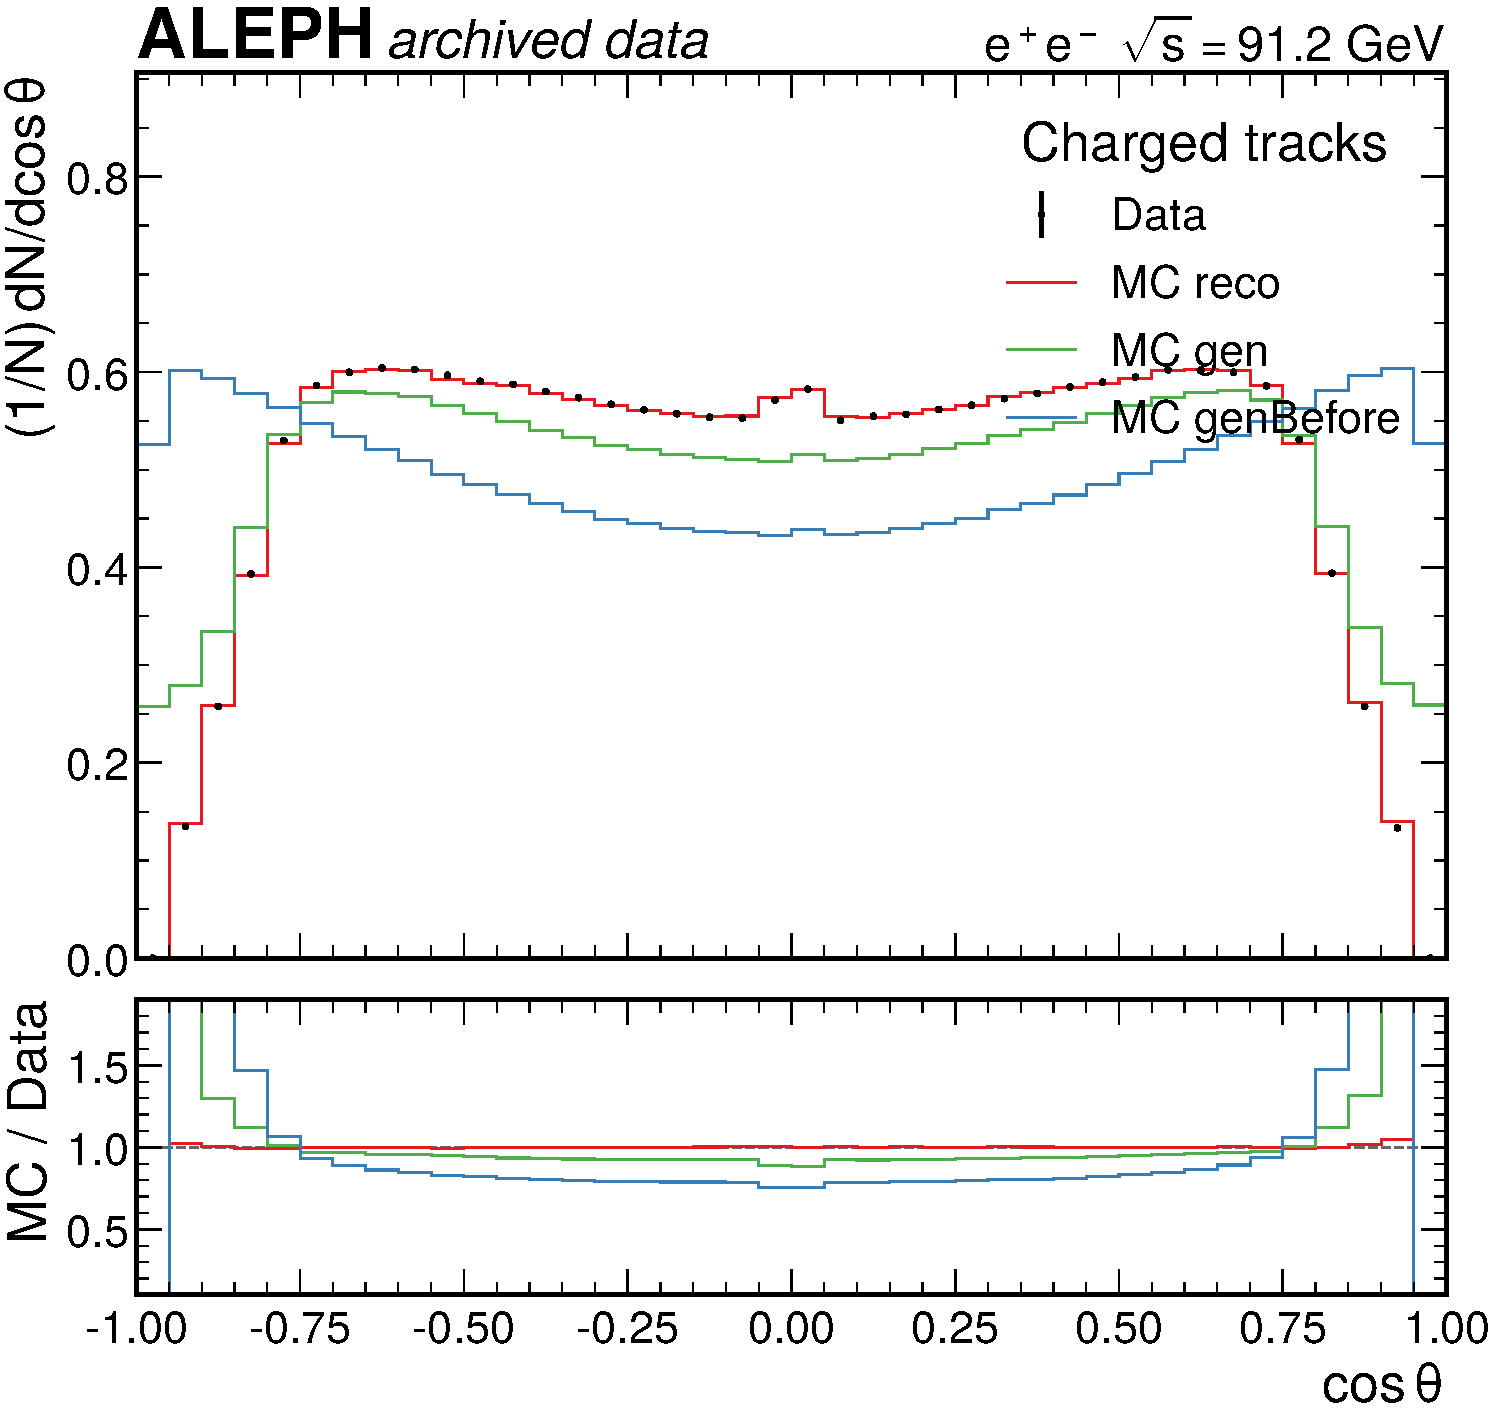
\includegraphics[width=0.242\textwidth]{figures/pwflag0_cosTheta.pdf}
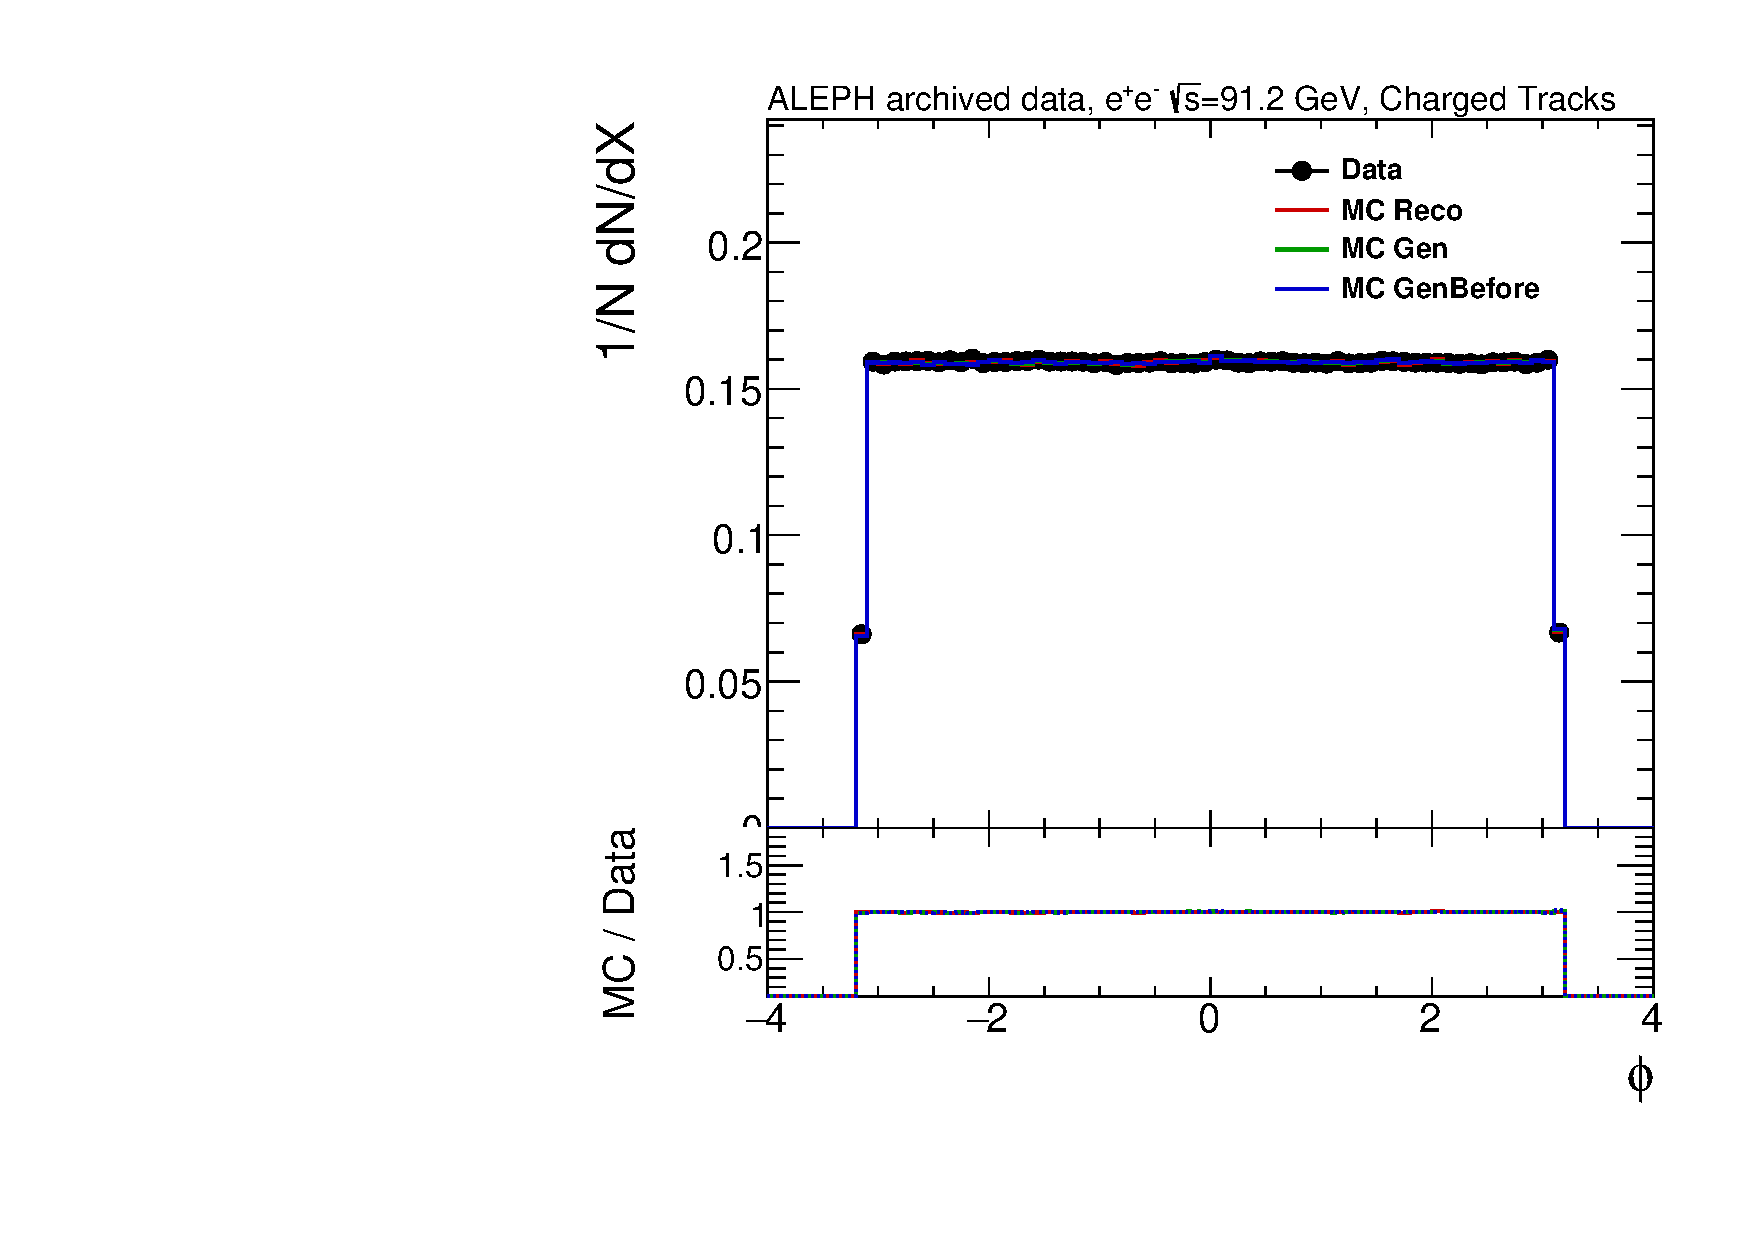
\includegraphics[width=0.242\textwidth]{figures/pwflag0_phi.pdf}
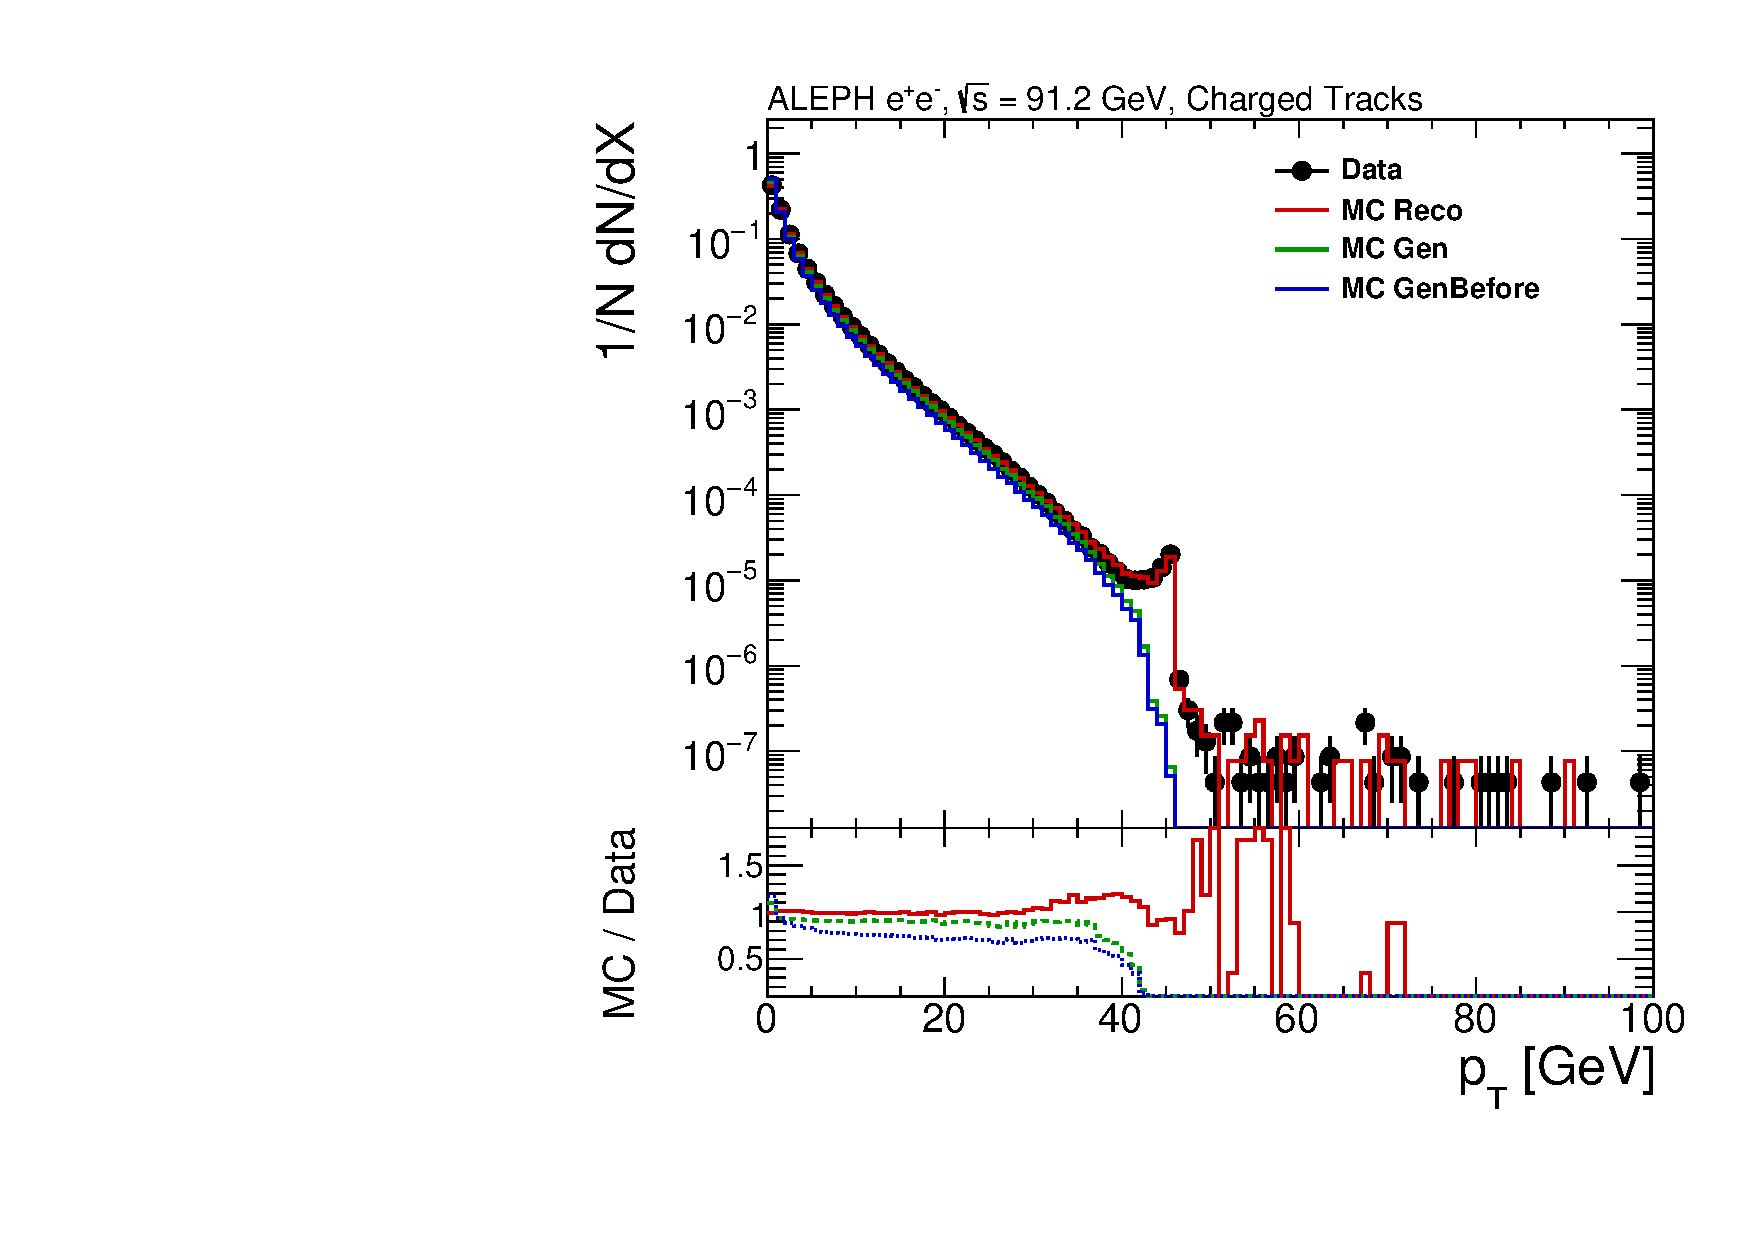
\includegraphics[width=0.242\textwidth]{figures/pwflag0_pt.pdf}
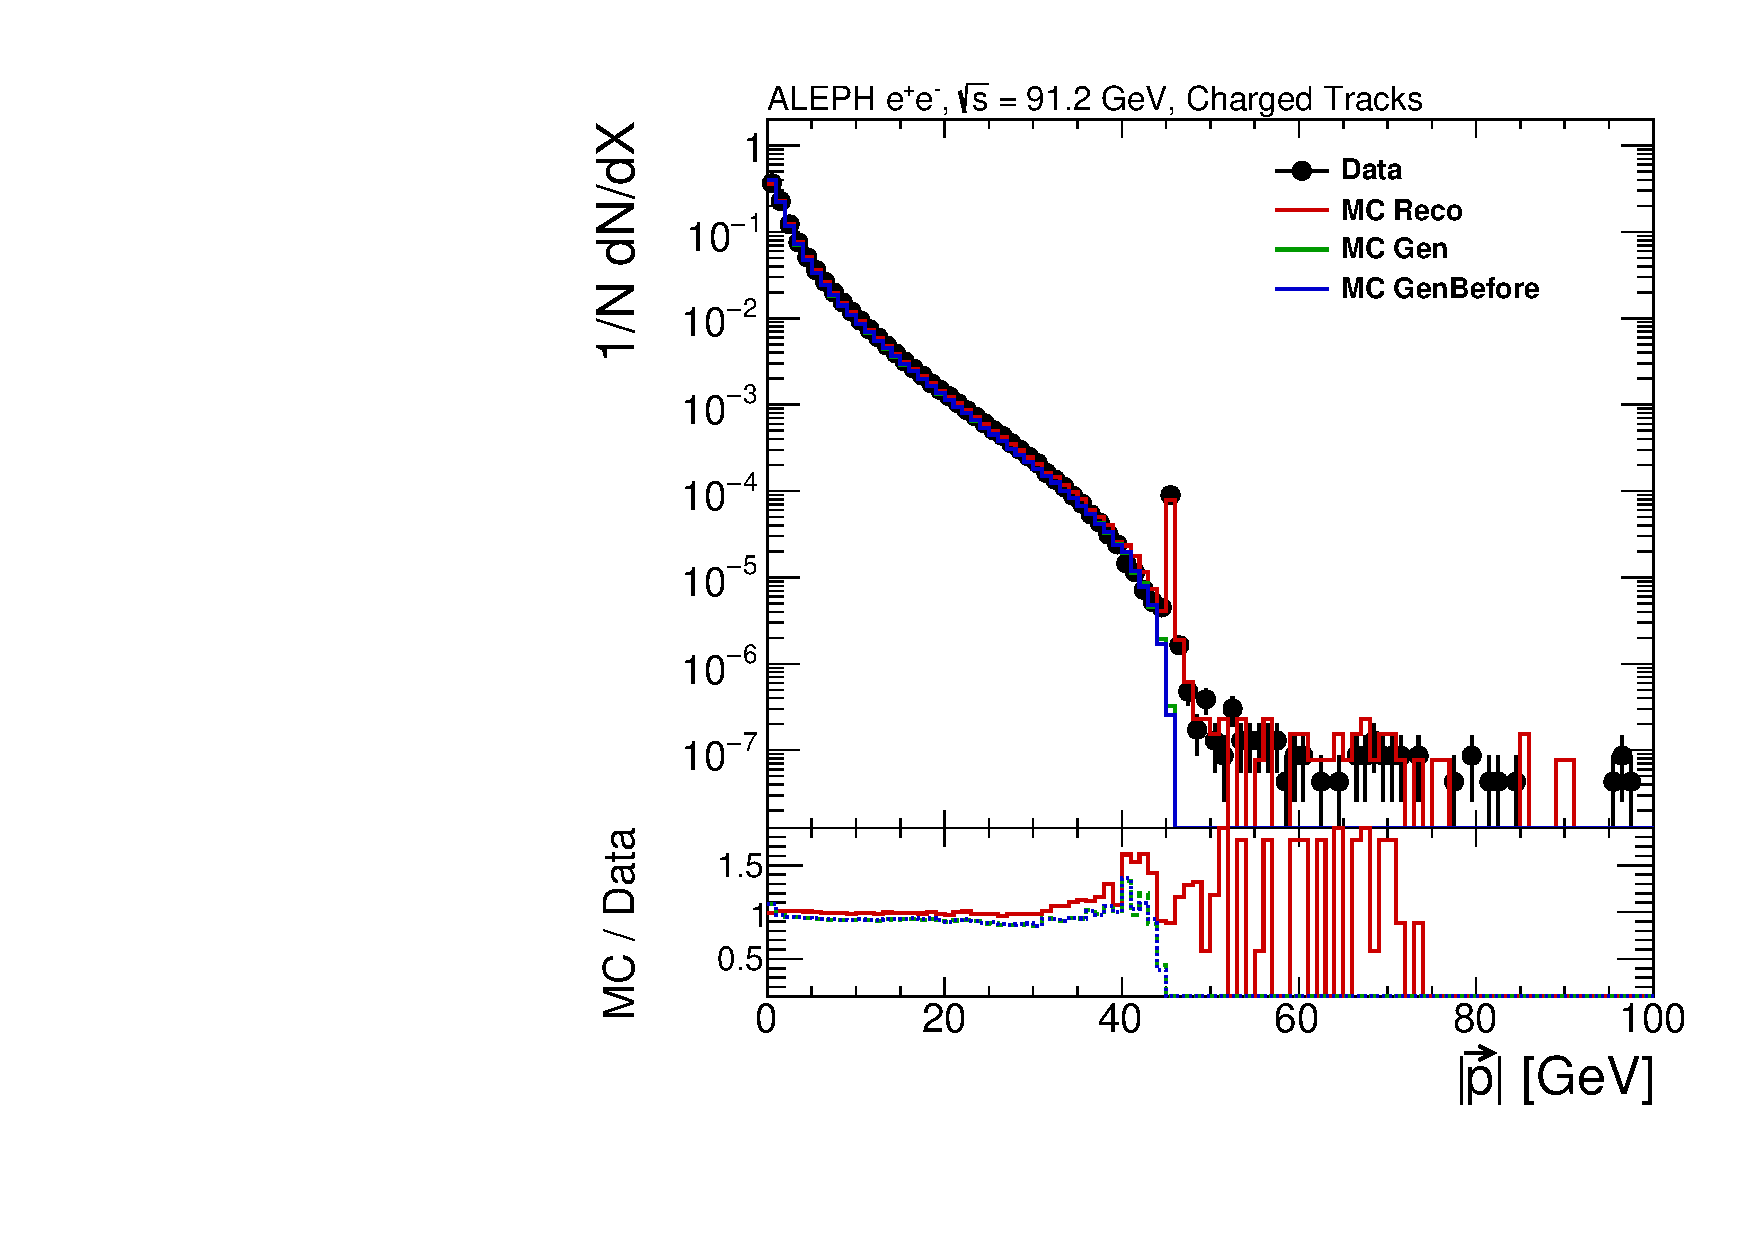
\includegraphics[width=0.242\textwidth]{figures/pwflag0_pmag.pdf}
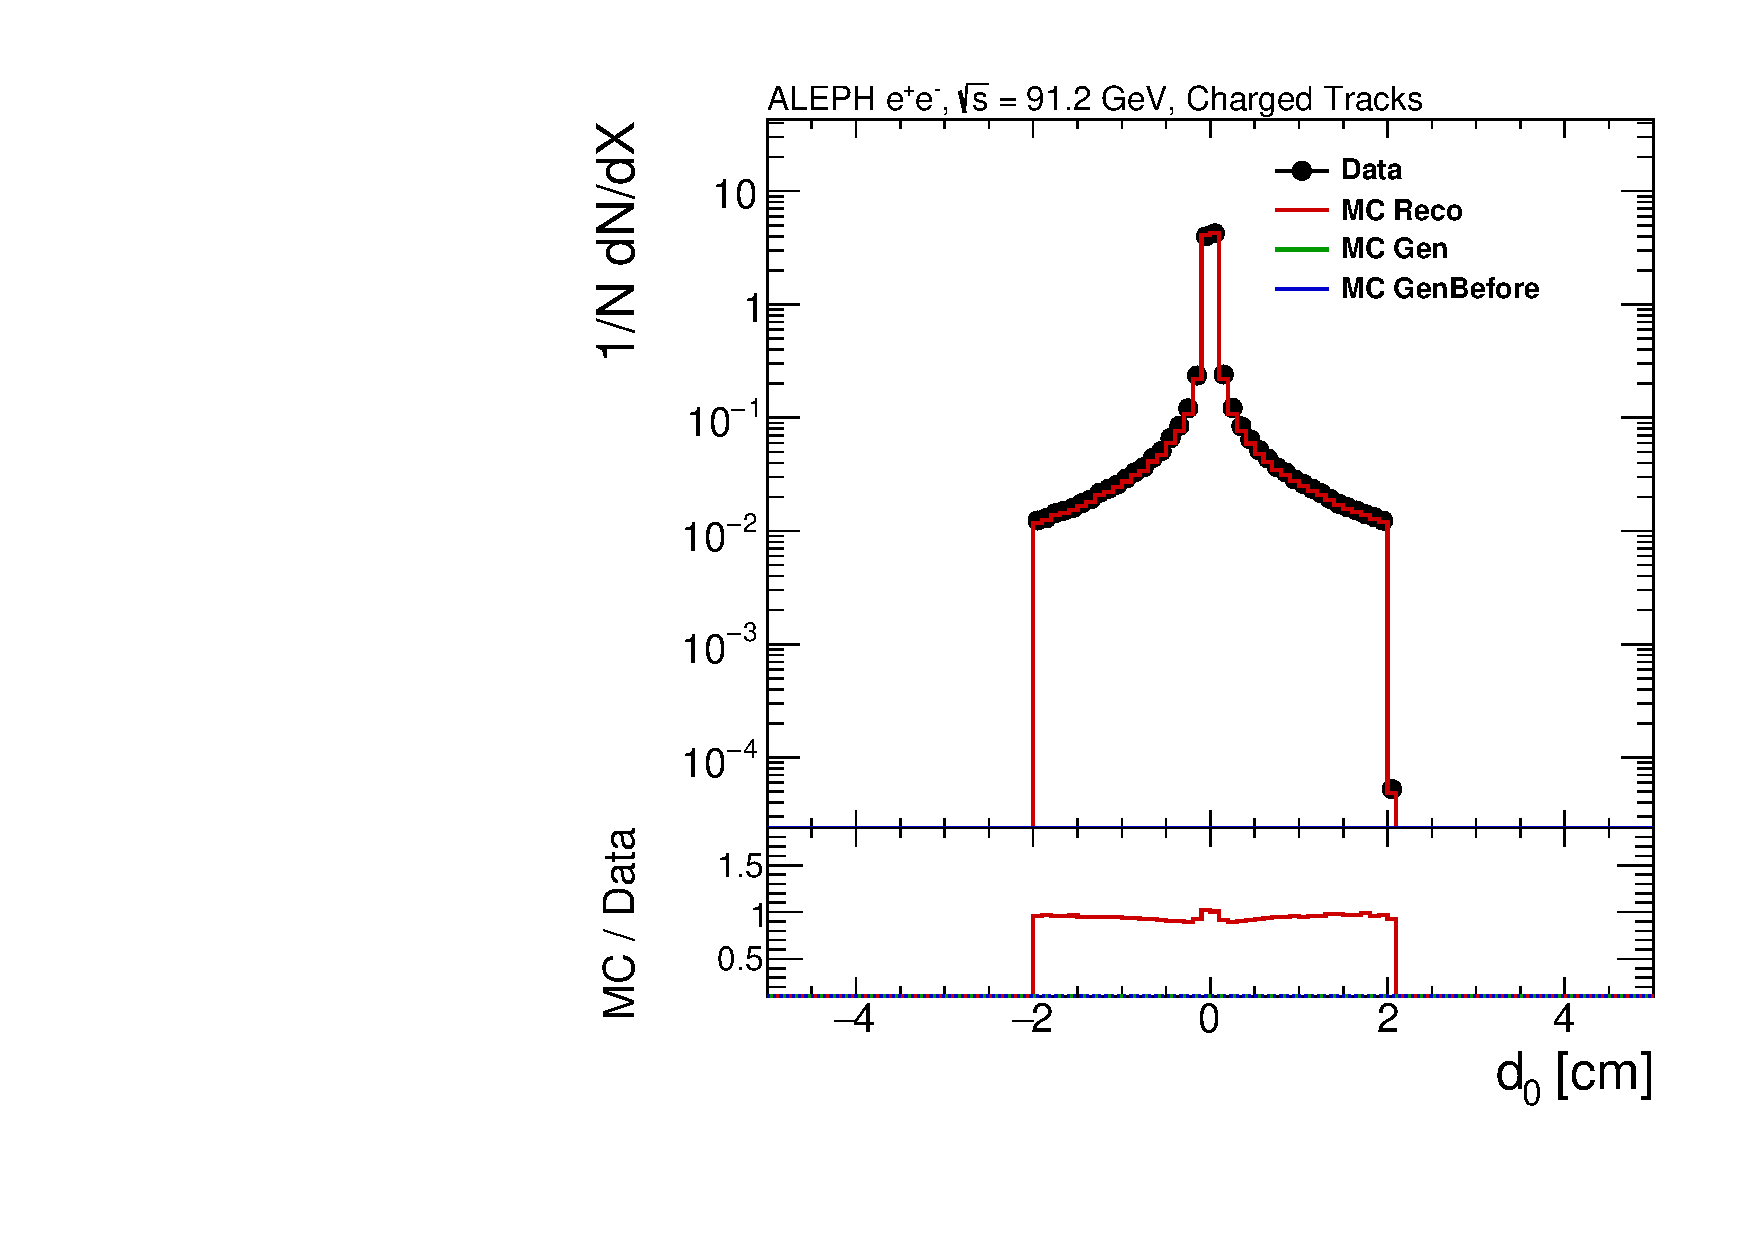
\includegraphics[width=0.242\textwidth]{figures/pwflag0_d0.pdf}
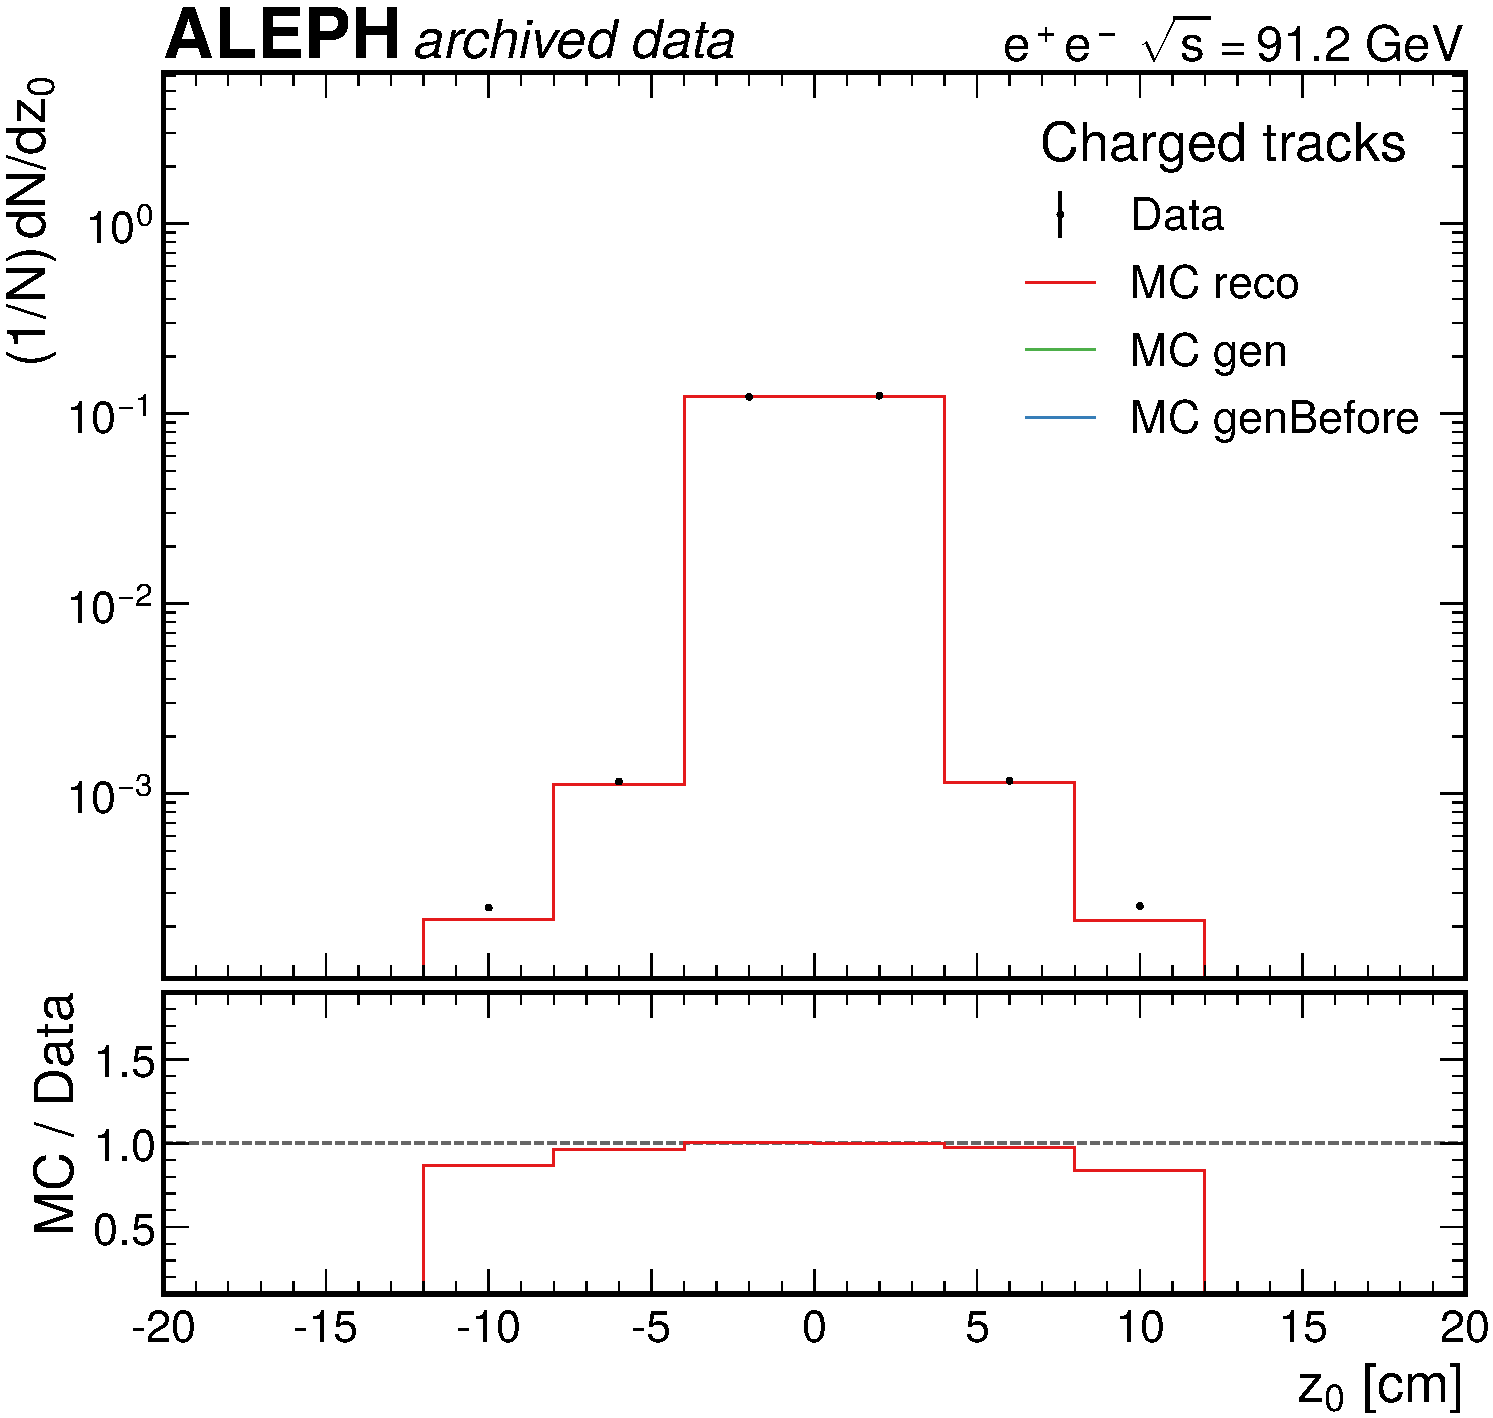
\includegraphics[width=0.242\textwidth]{figures/pwflag0_z0.pdf}
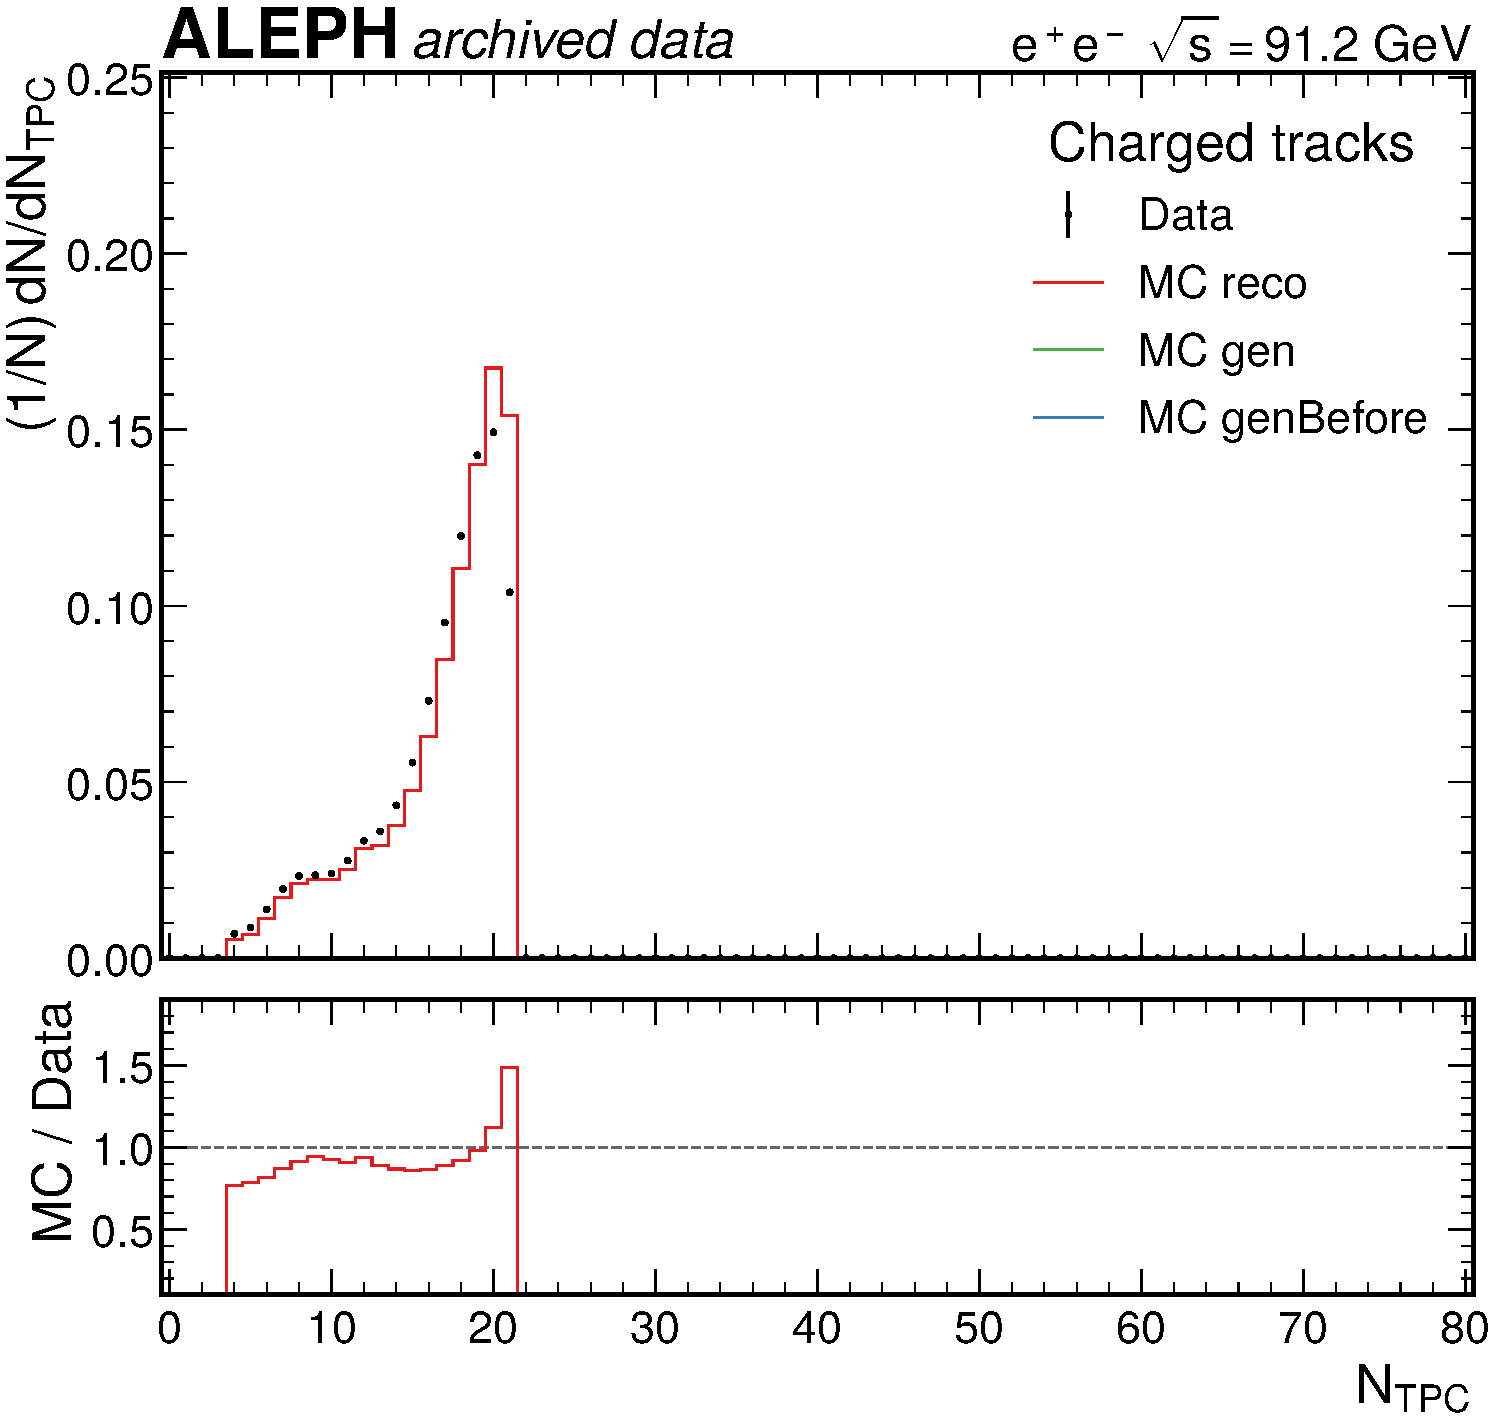
\includegraphics[width=0.242\textwidth]{figures/pwflag0_ntpc.pdf}
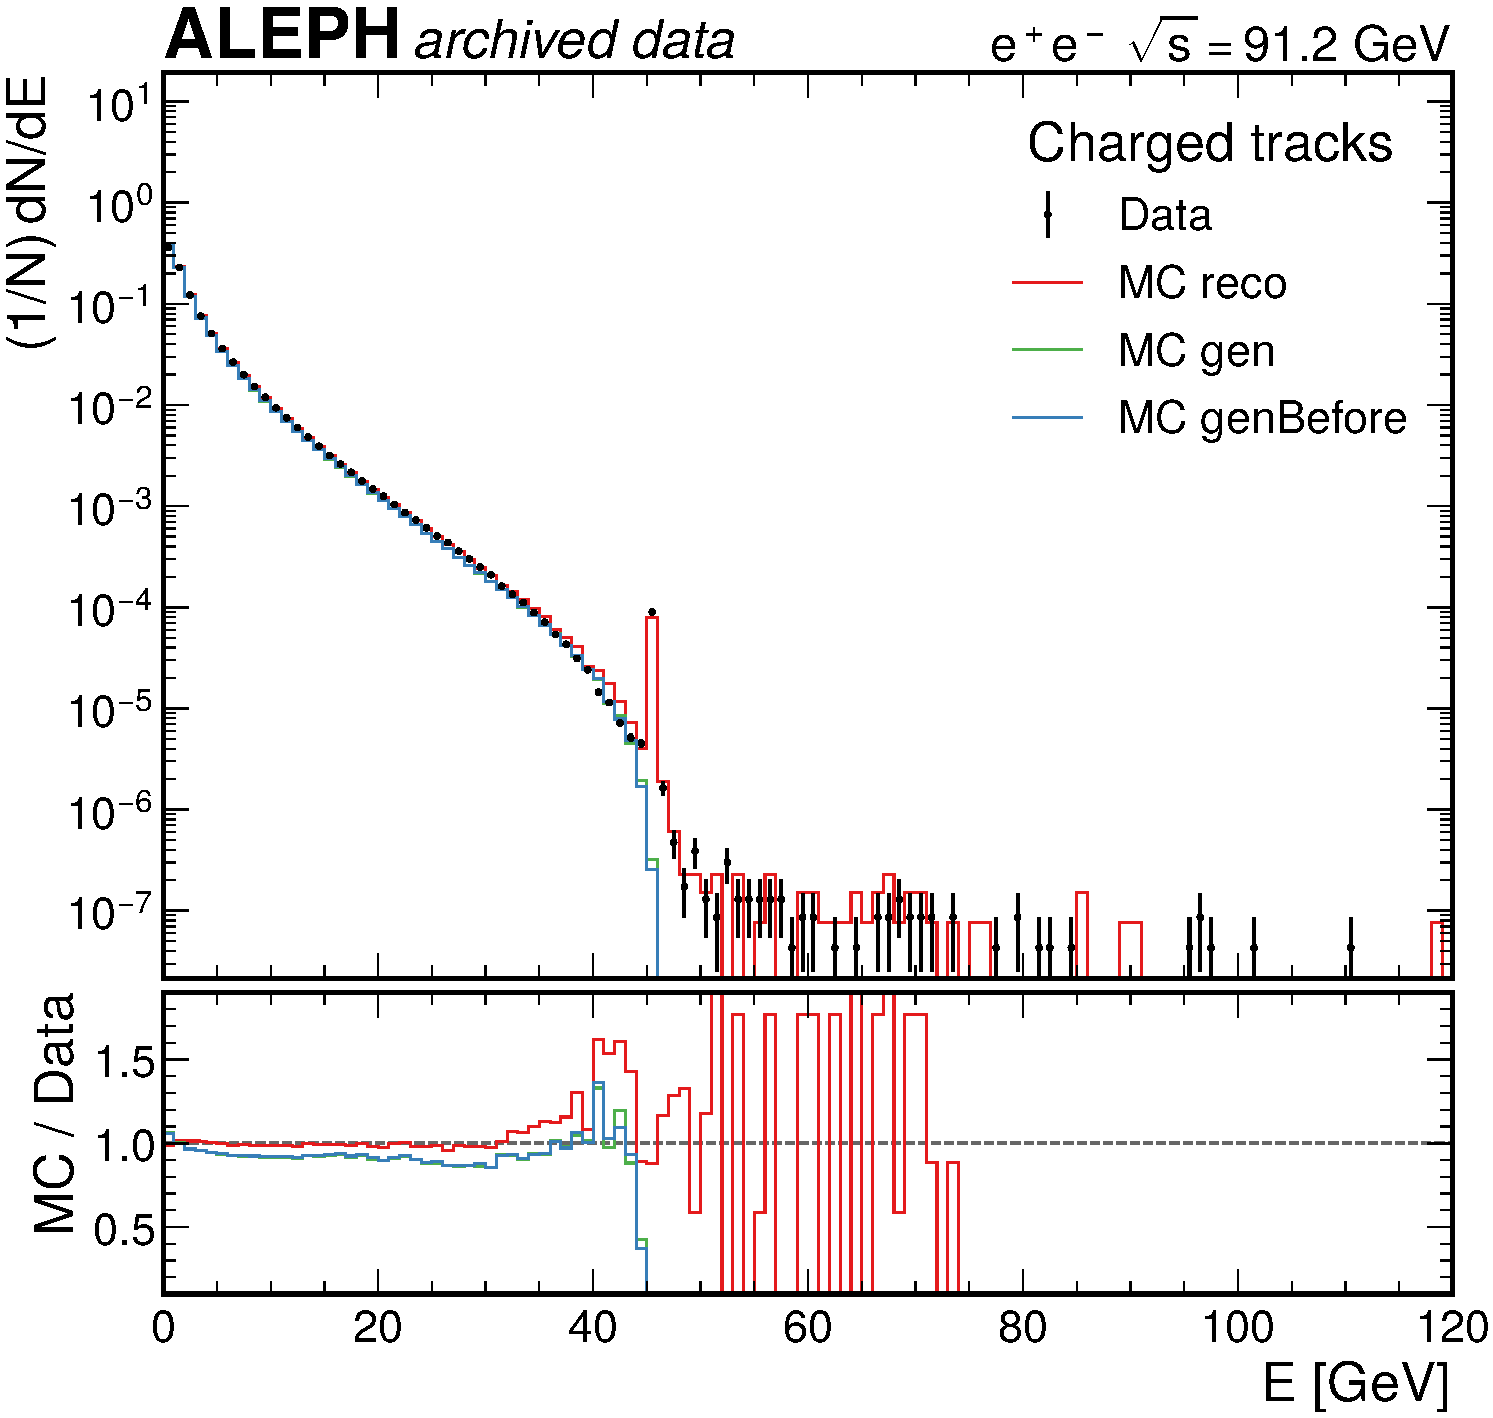
\includegraphics[width=0.242\textwidth]{figures/pwflag0_energy.pdf}
% 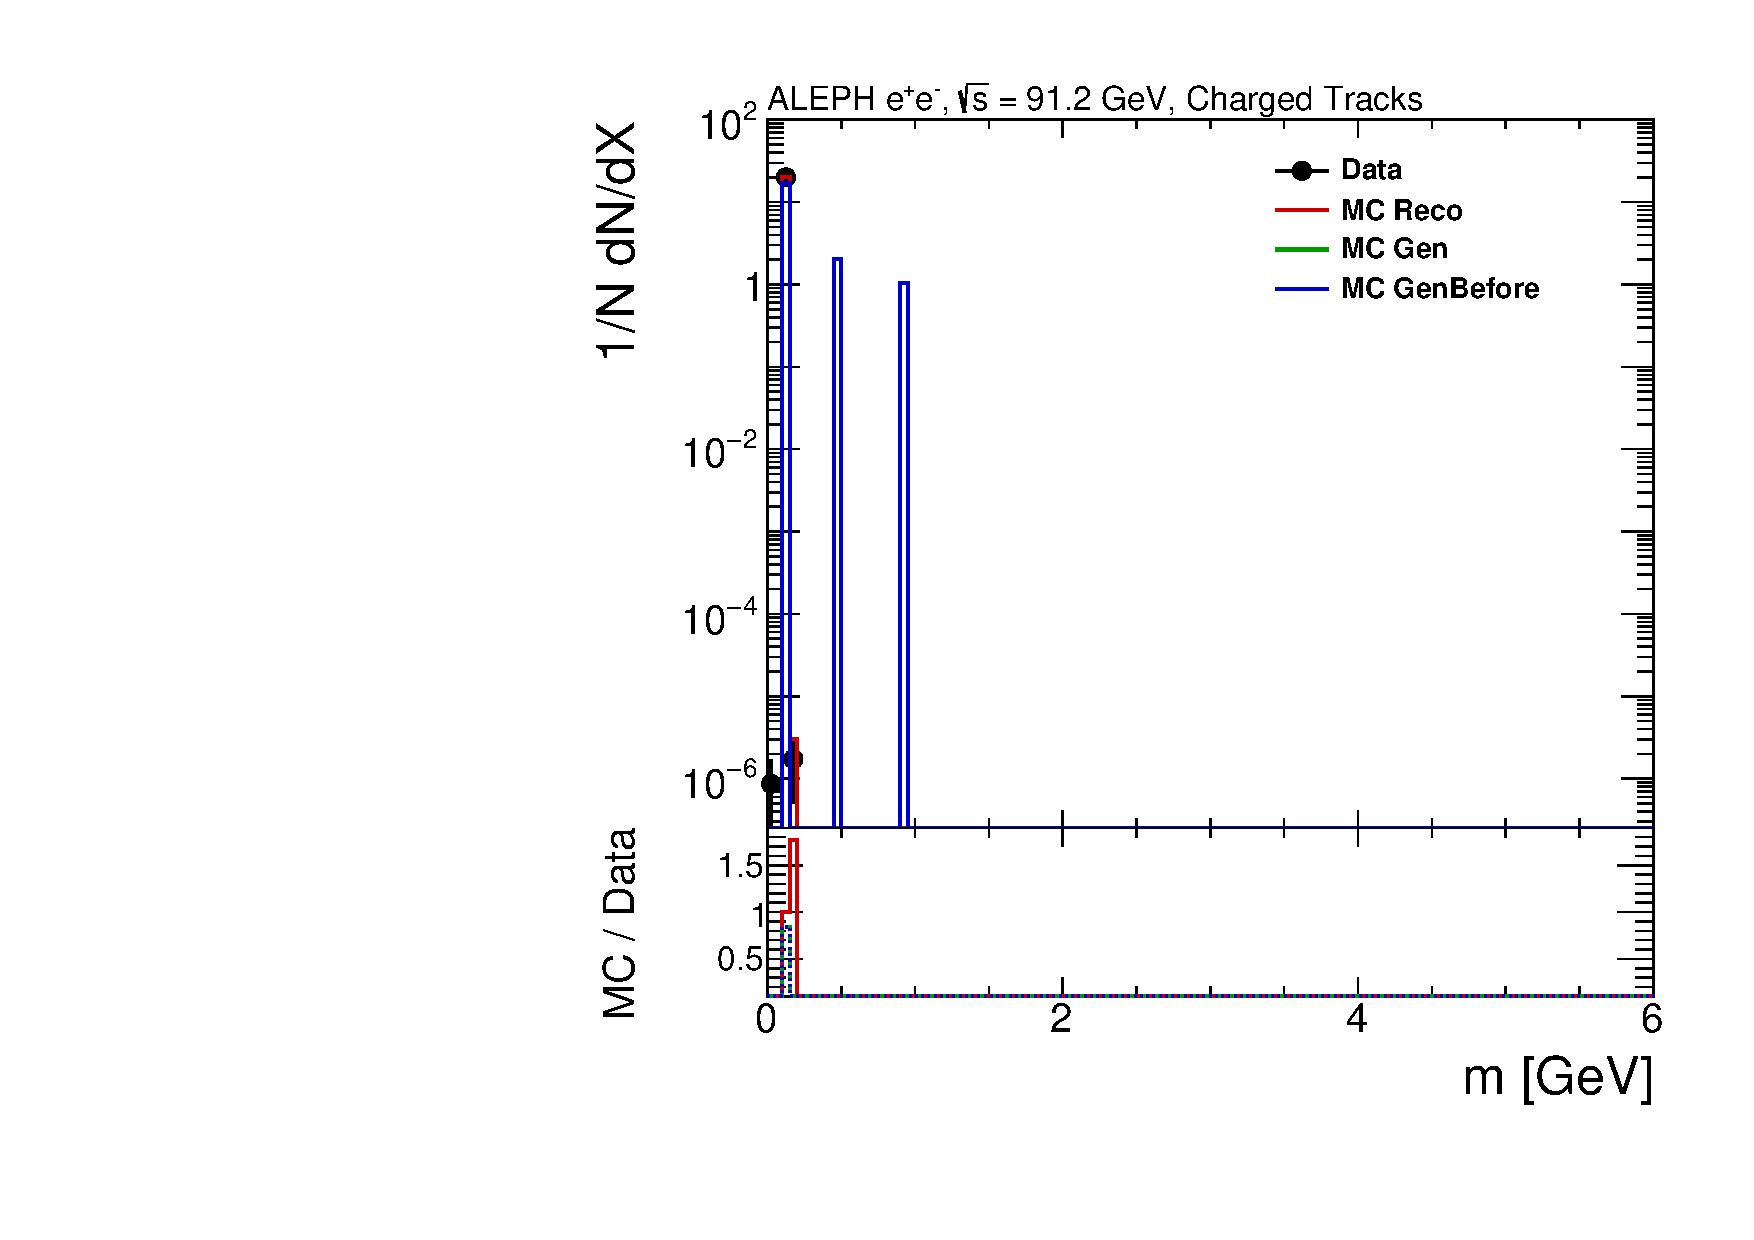
\includegraphics[width=0.242\textwidth]{figures/pwflag0_mass.pdf}
\caption{Complete \texttt{pwflag}=0 kinematic set.}
\label{fig:pwflag0_full}
\end{figure}

\begin{figure}[t!]
\centering
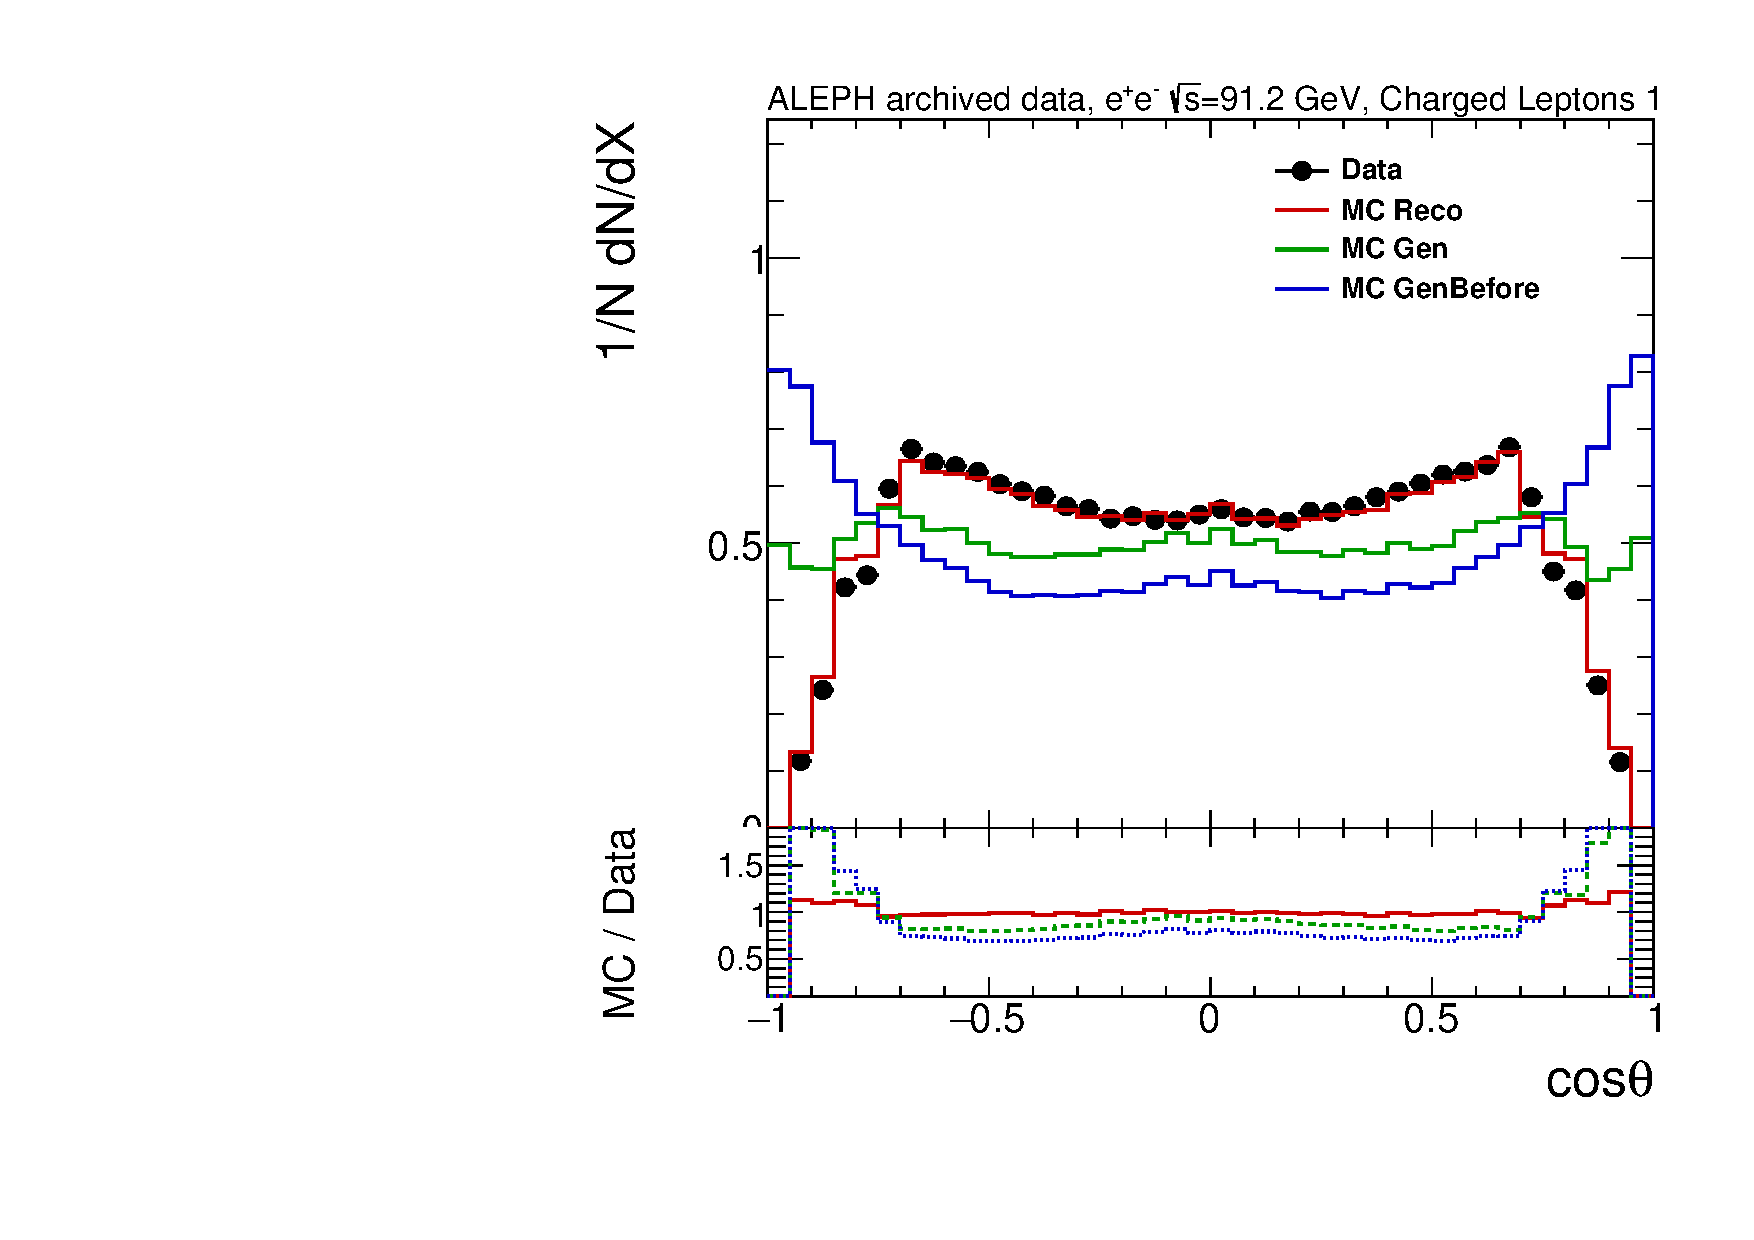
\includegraphics[width=0.242\textwidth]{figures/pwflag1_cosTheta.pdf}
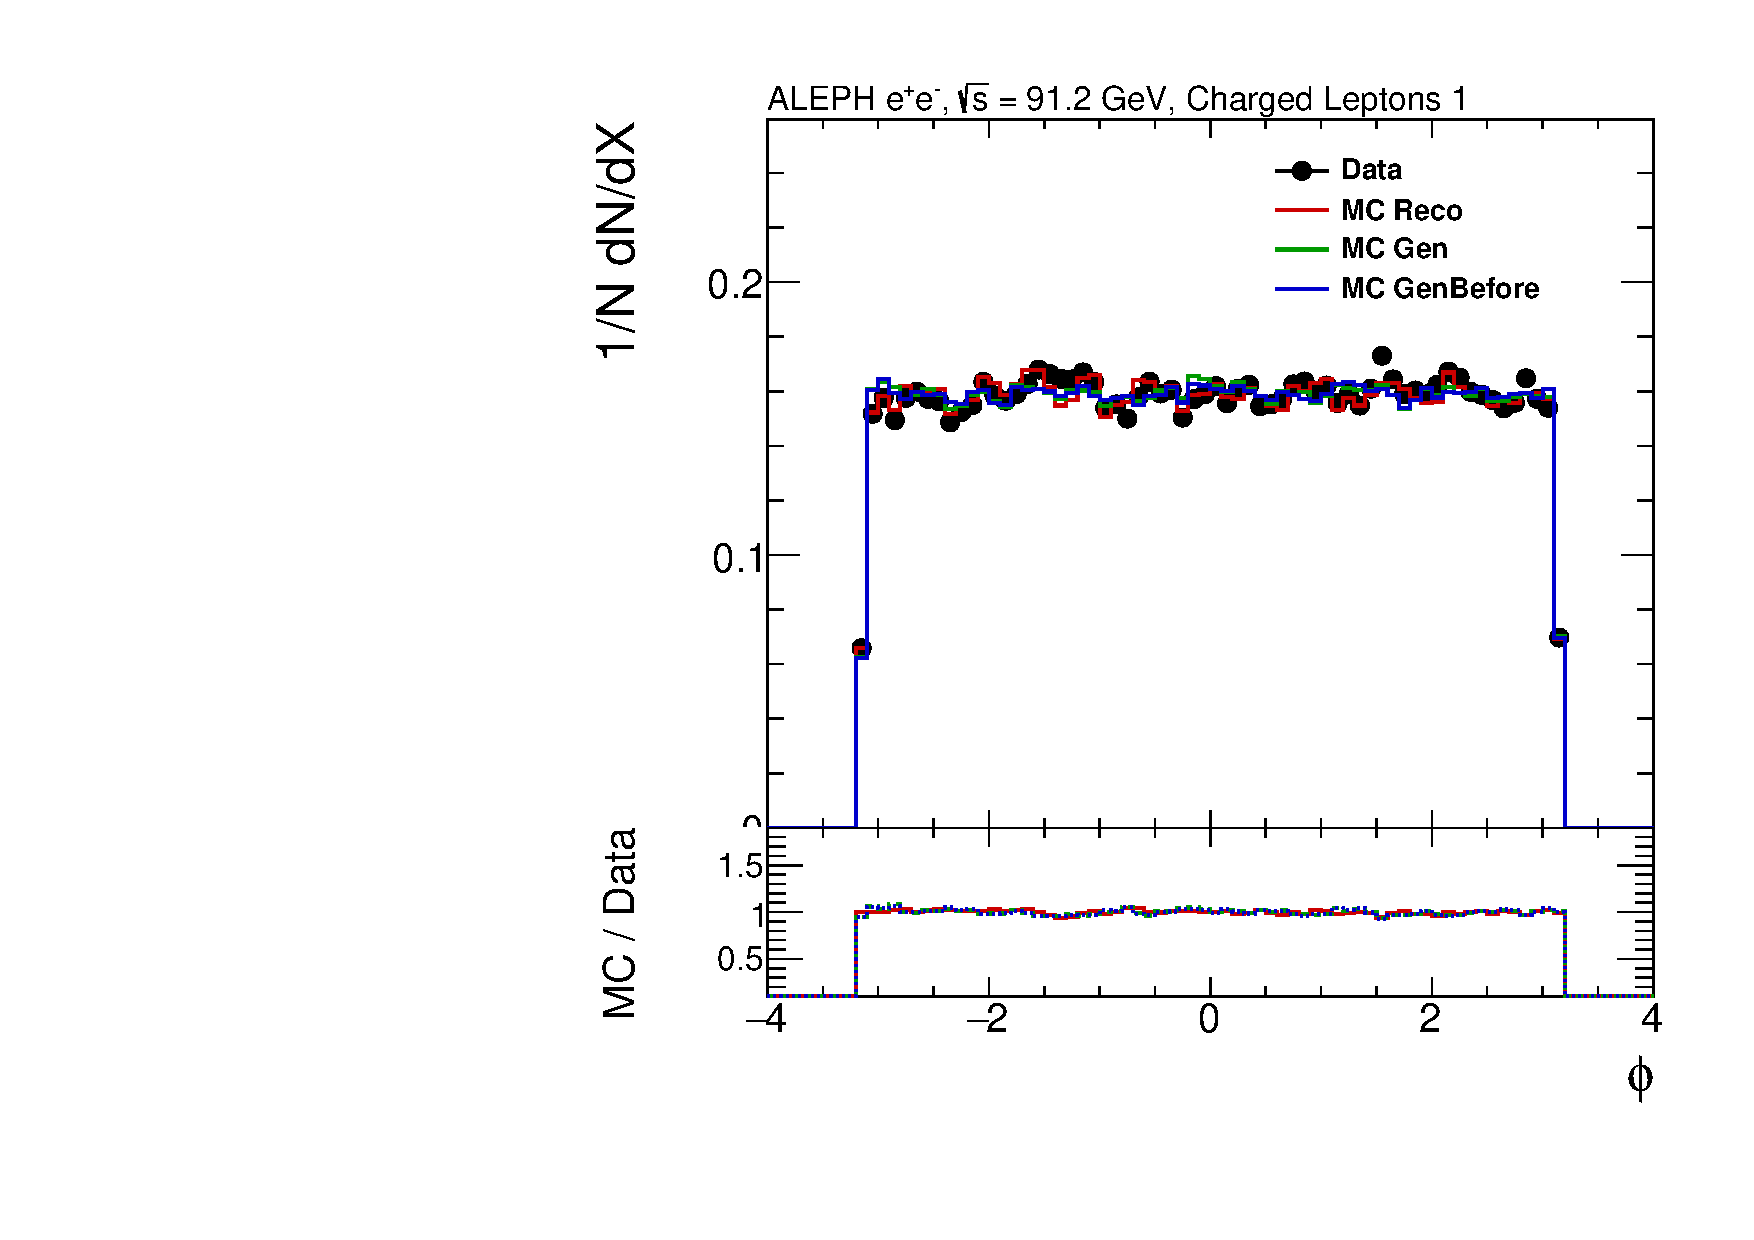
\includegraphics[width=0.242\textwidth]{figures/pwflag1_phi.pdf}
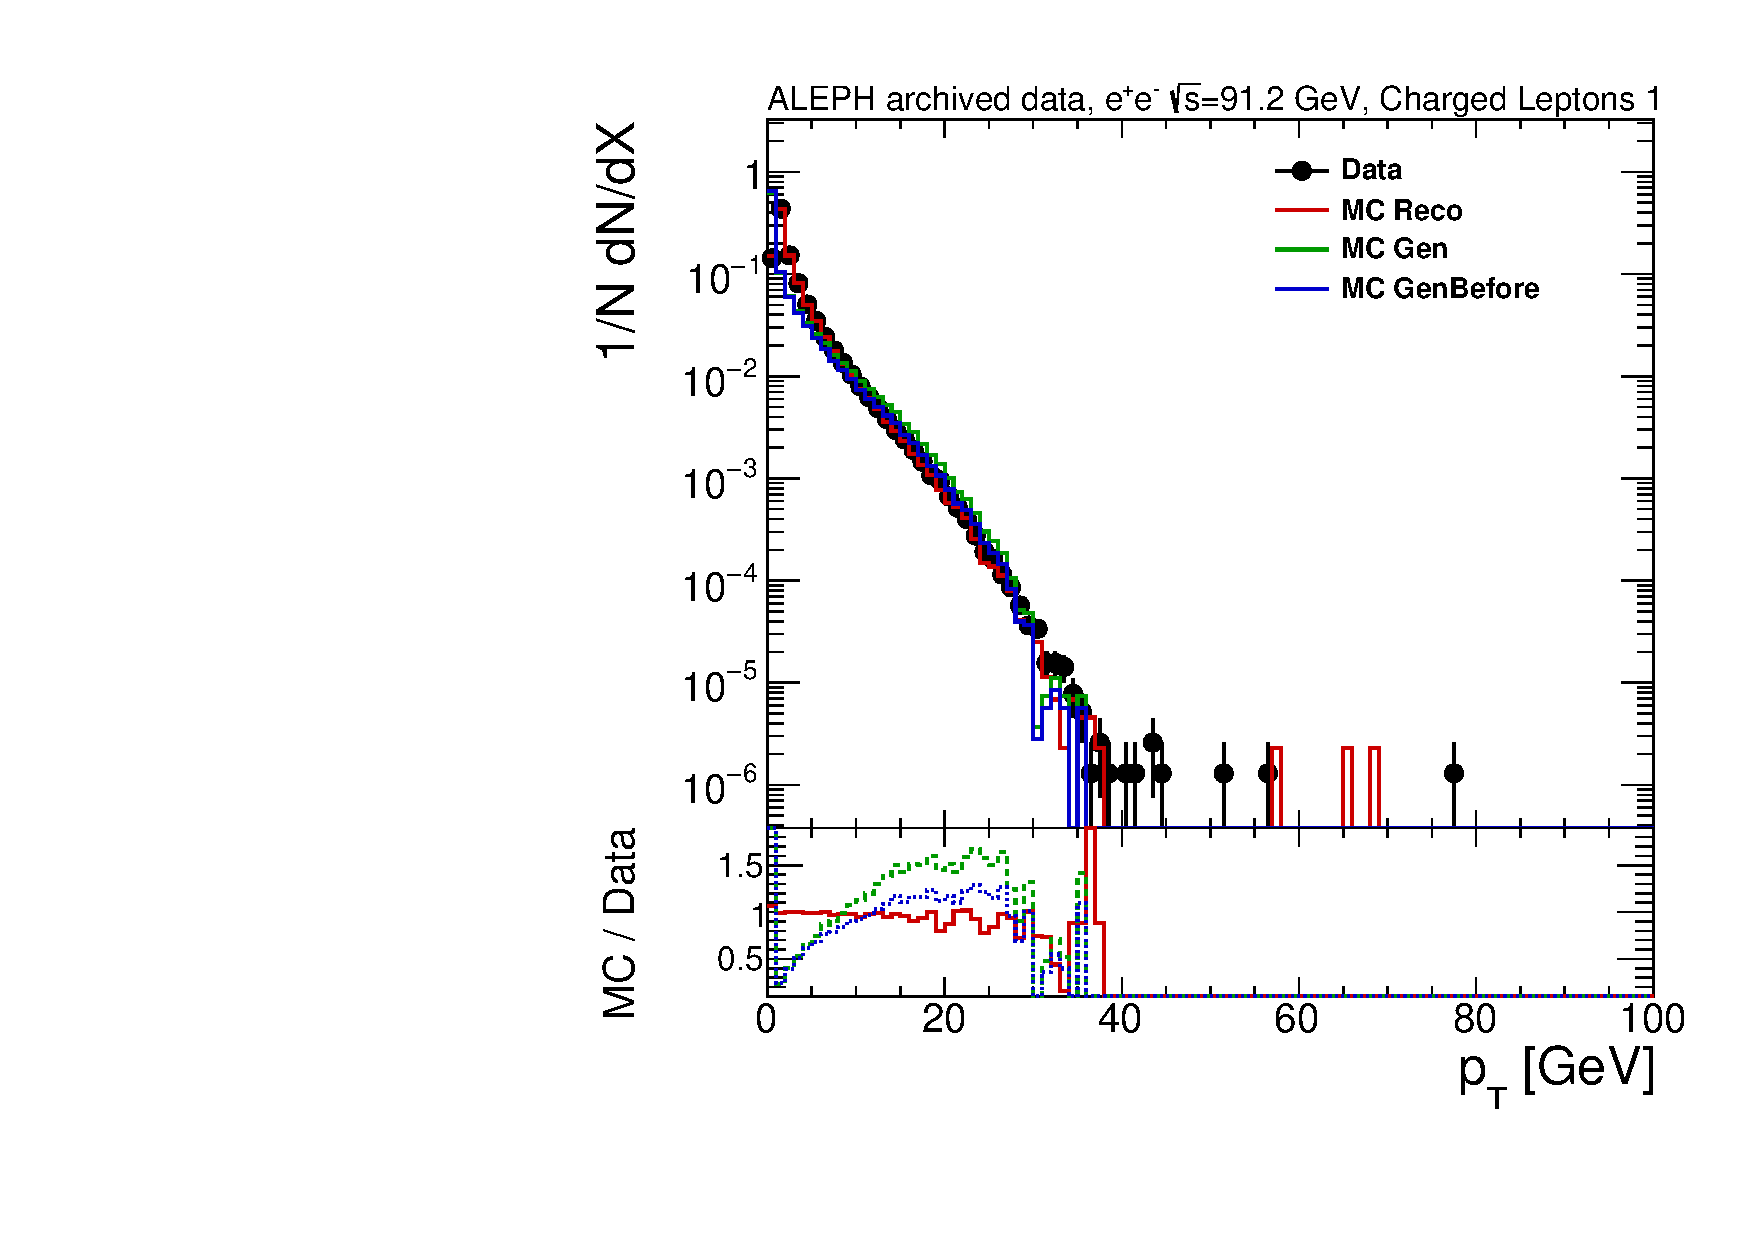
\includegraphics[width=0.242\textwidth]{figures/pwflag1_pt.pdf}
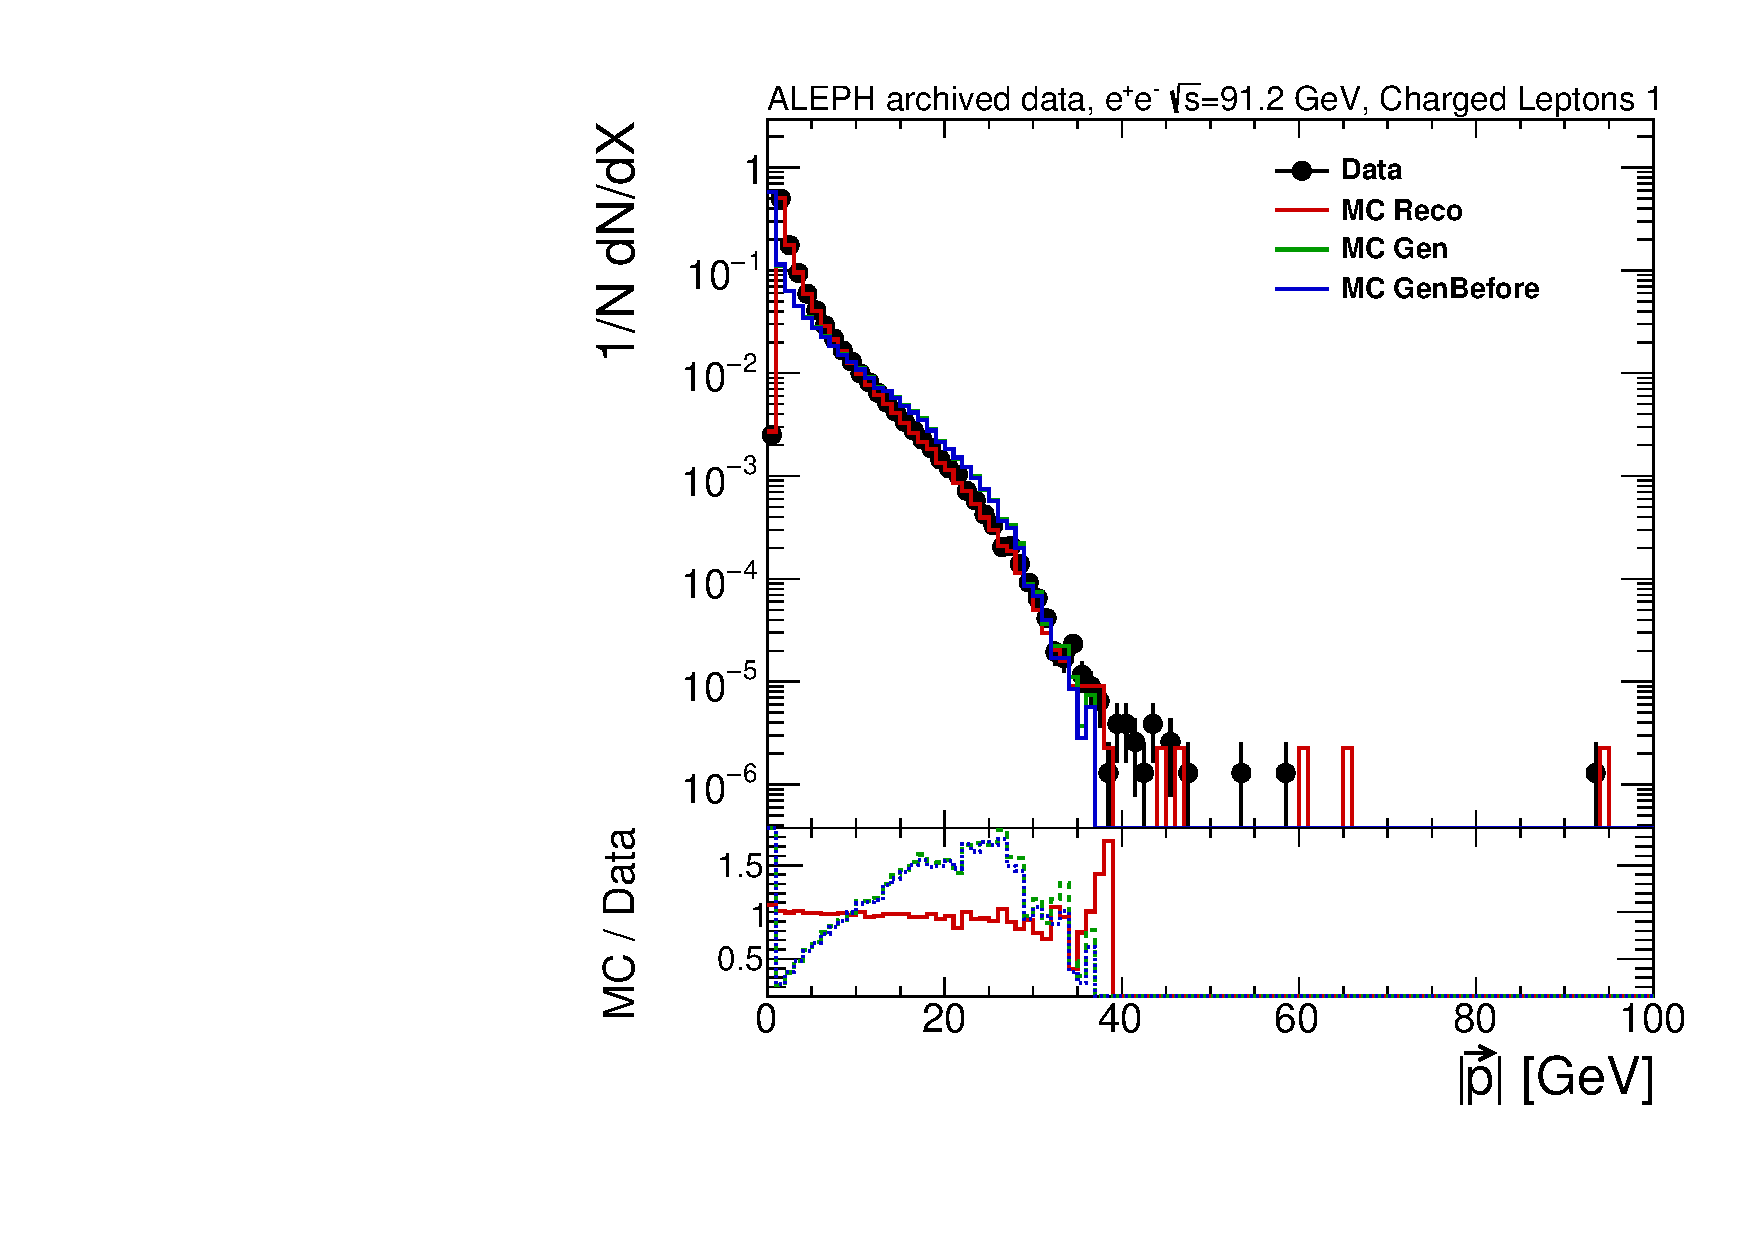
\includegraphics[width=0.242\textwidth]{figures/pwflag1_pmag.pdf}
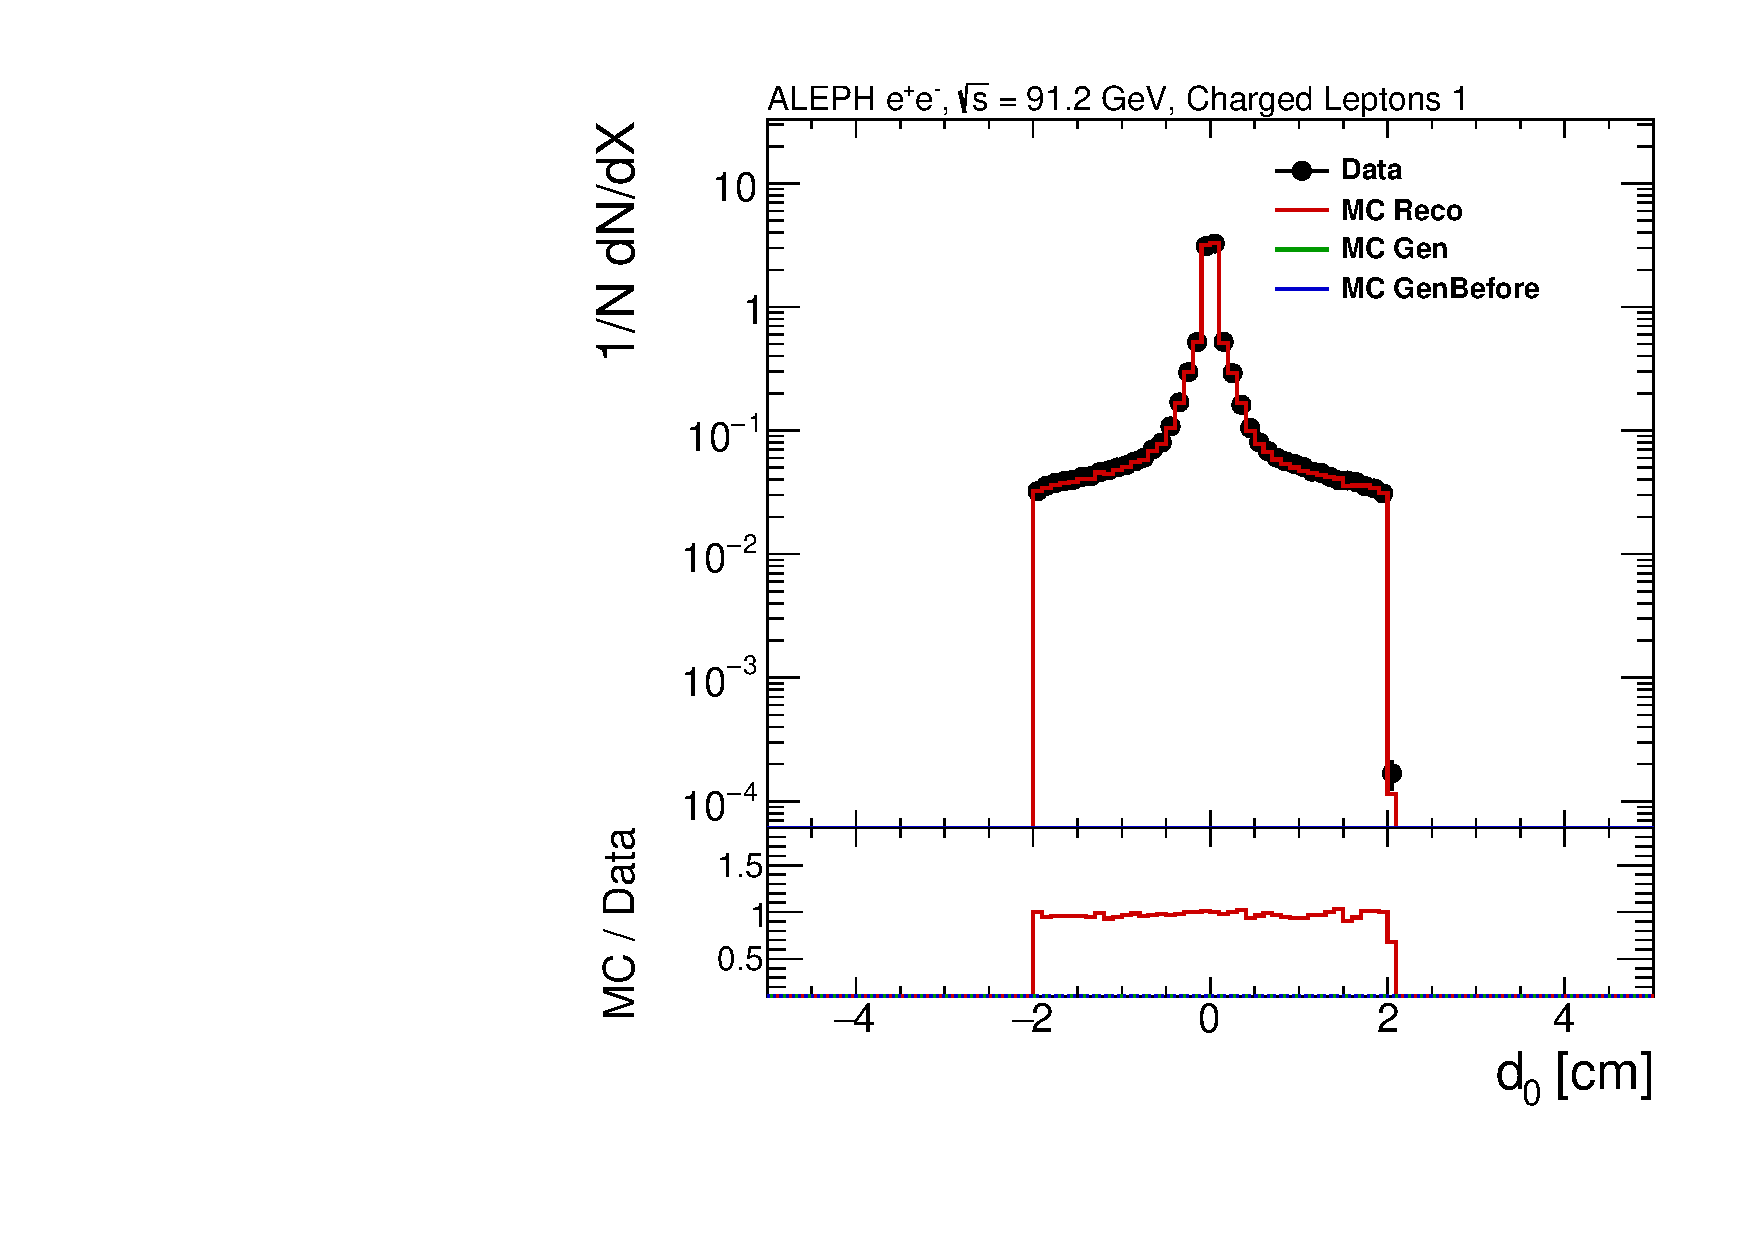
\includegraphics[width=0.242\textwidth]{figures/pwflag1_d0.pdf}
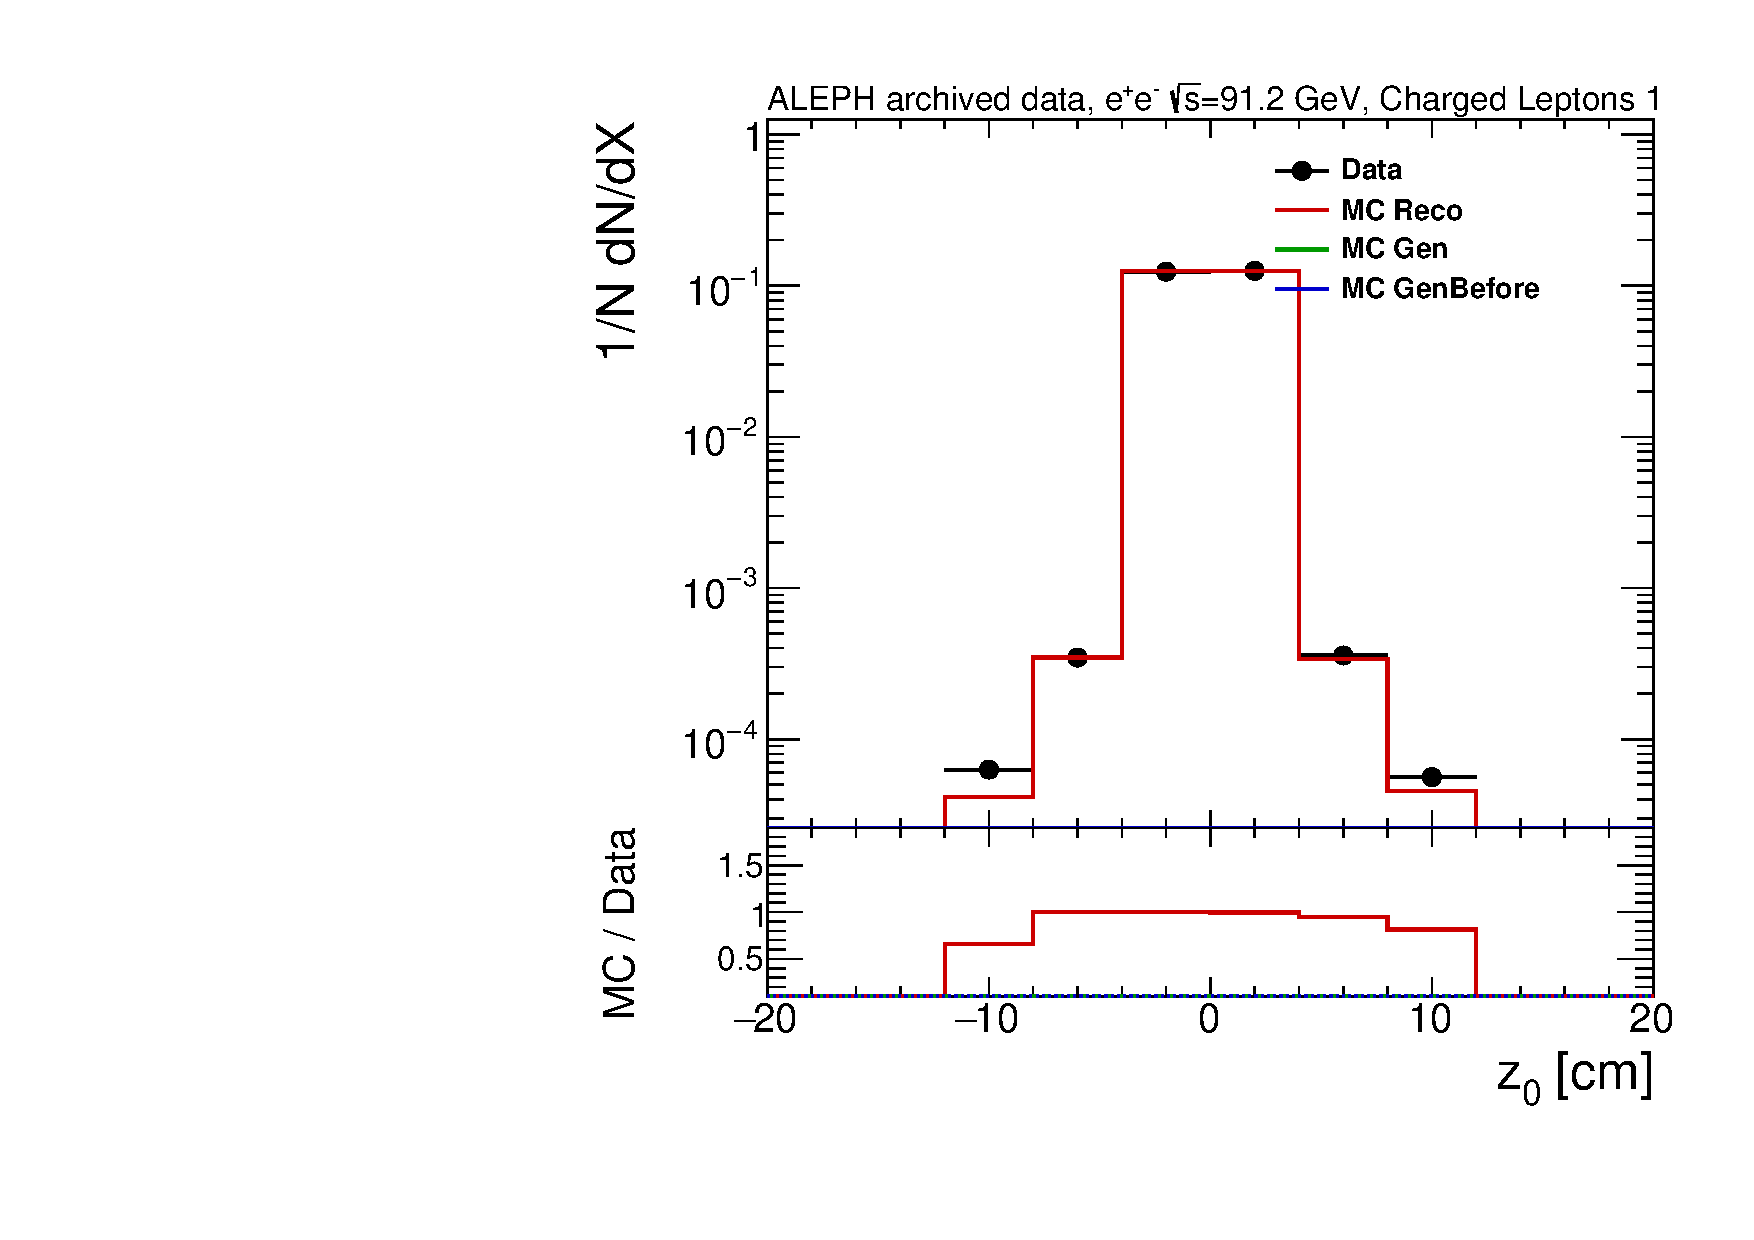
\includegraphics[width=0.242\textwidth]{figures/pwflag1_z0.pdf}
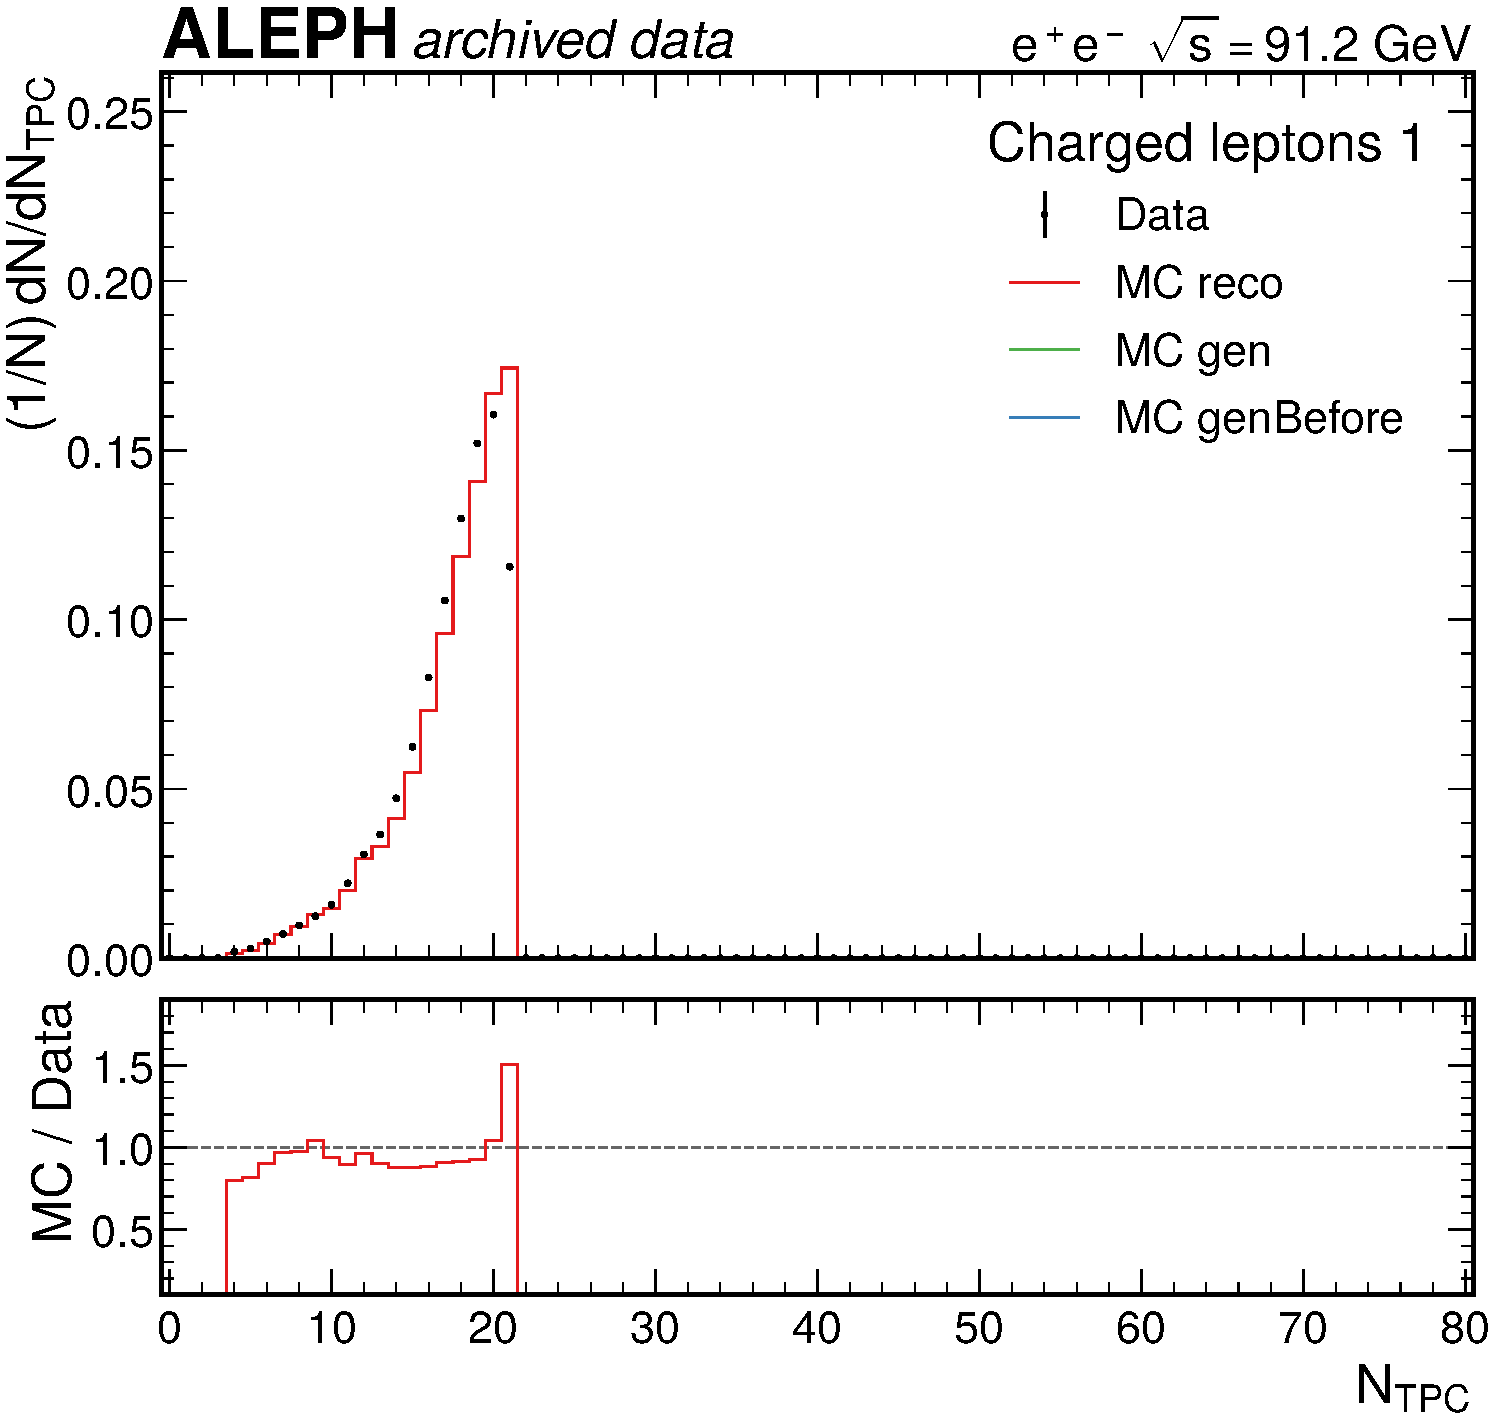
\includegraphics[width=0.242\textwidth]{figures/pwflag1_ntpc.pdf}
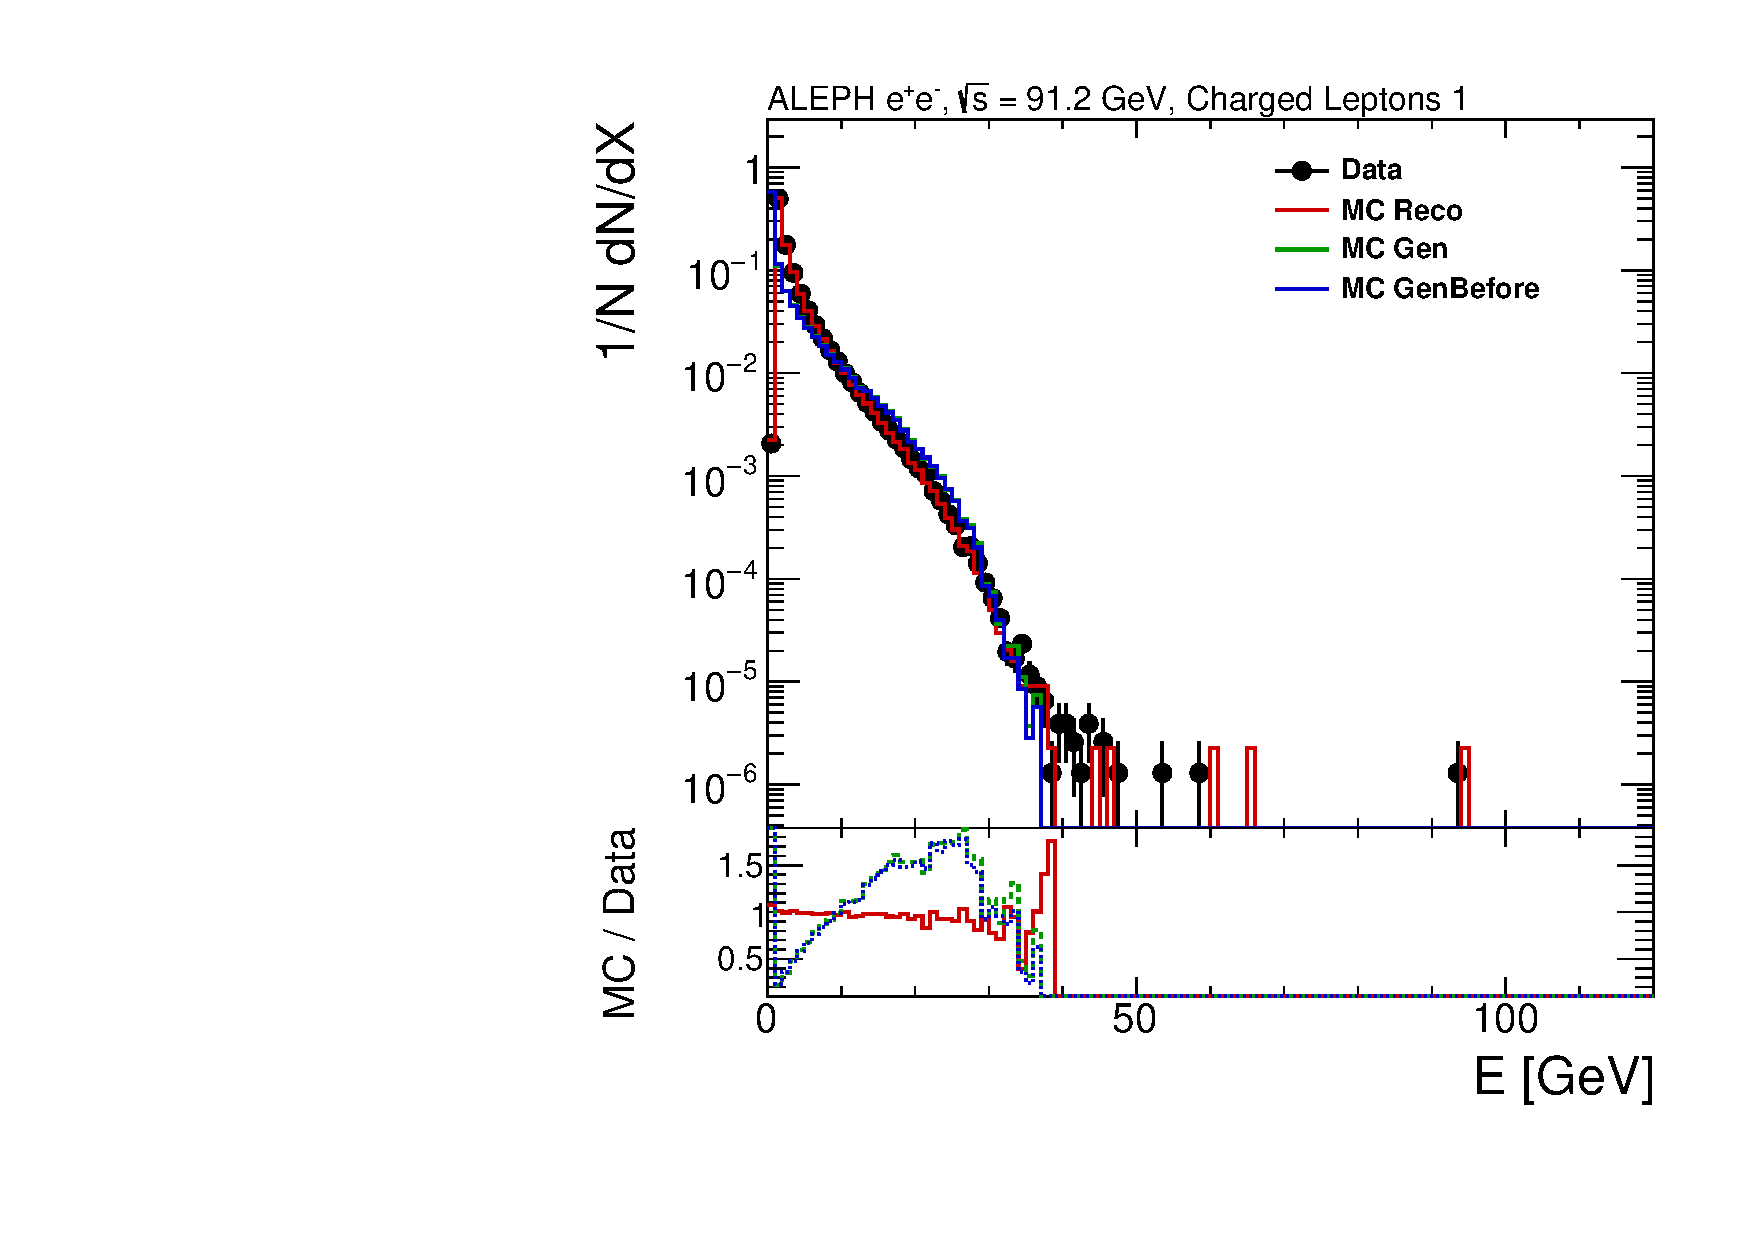
\includegraphics[width=0.242\textwidth]{figures/pwflag1_energy.pdf}
% 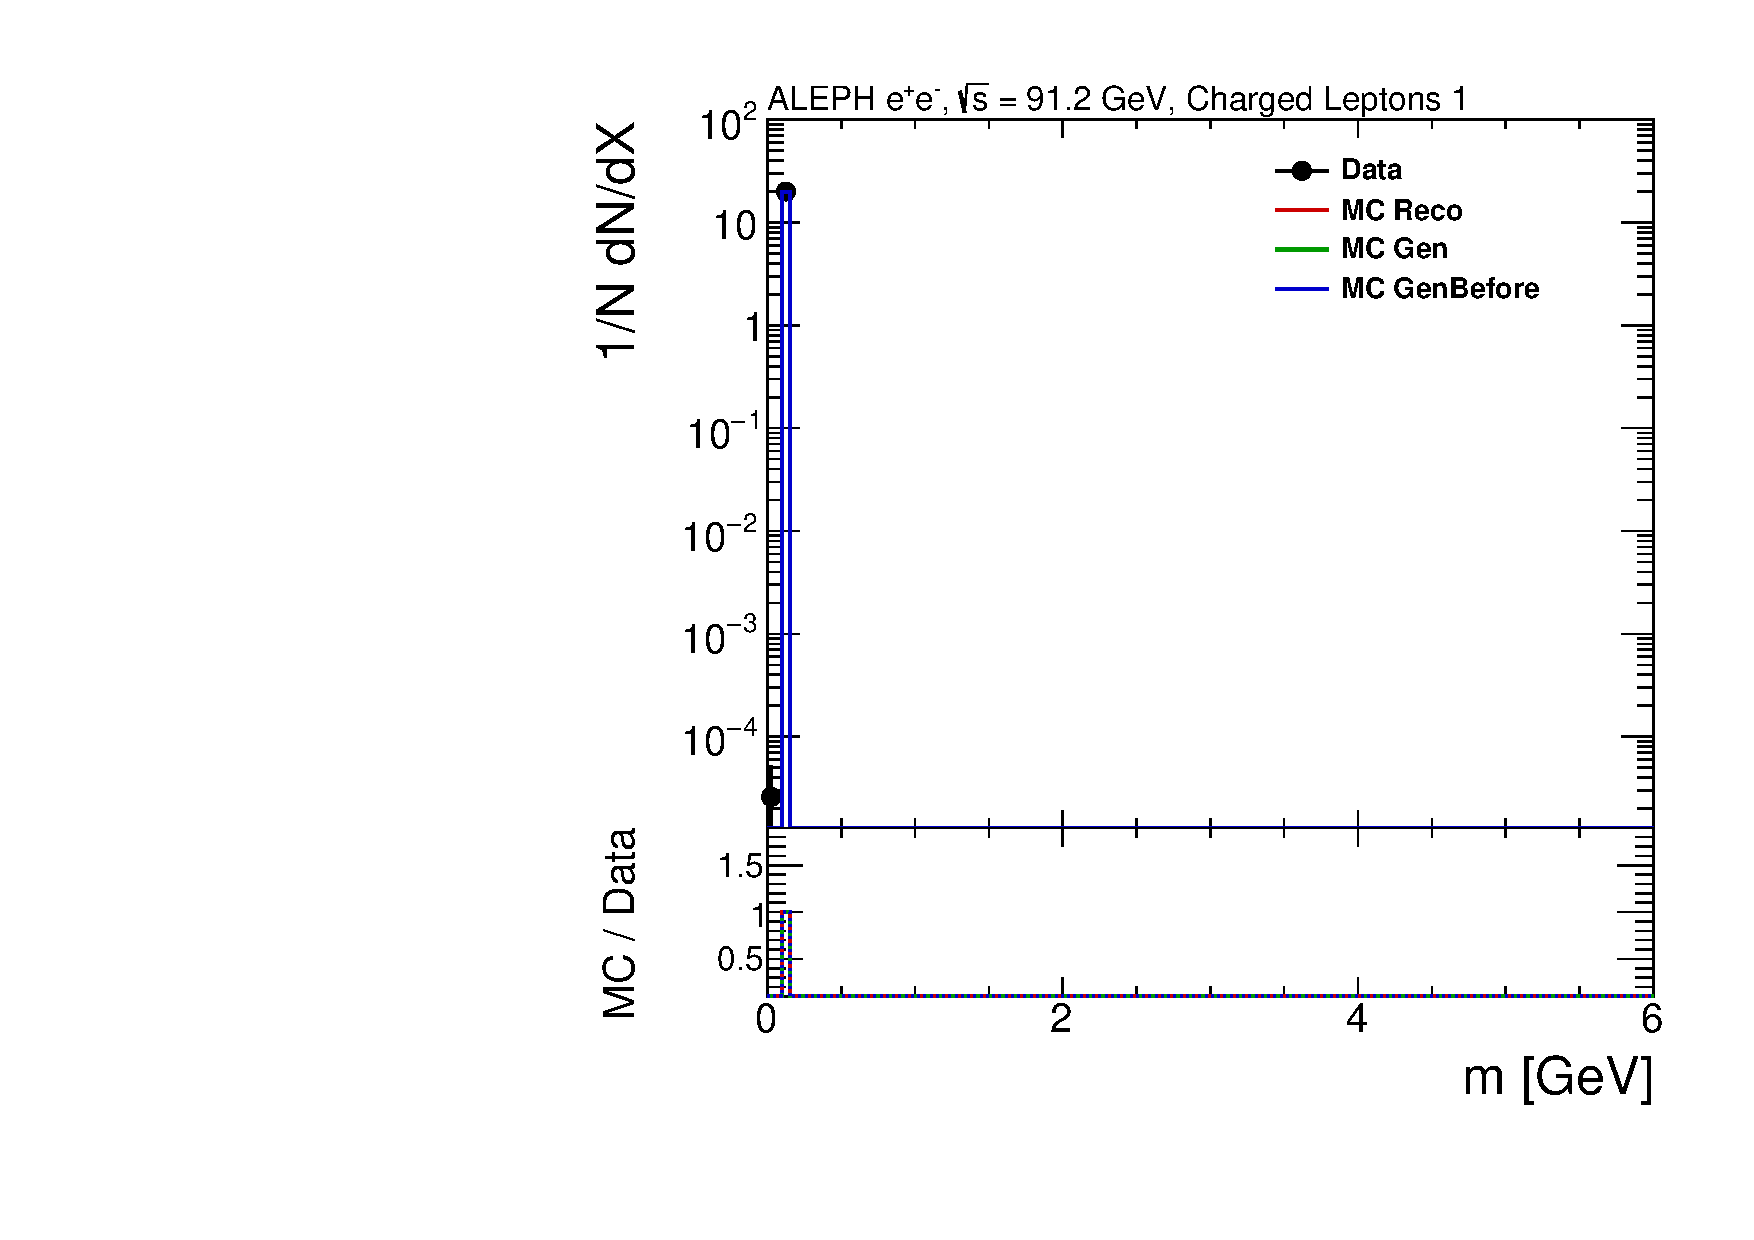
\includegraphics[width=0.242\textwidth]{figures/pwflag1_mass.pdf}
\caption{Complete \texttt{pwflag}=1 kinematic set.}
\label{fig:pwflag1_full}
\end{figure}

\begin{figure}[t!]
\centering
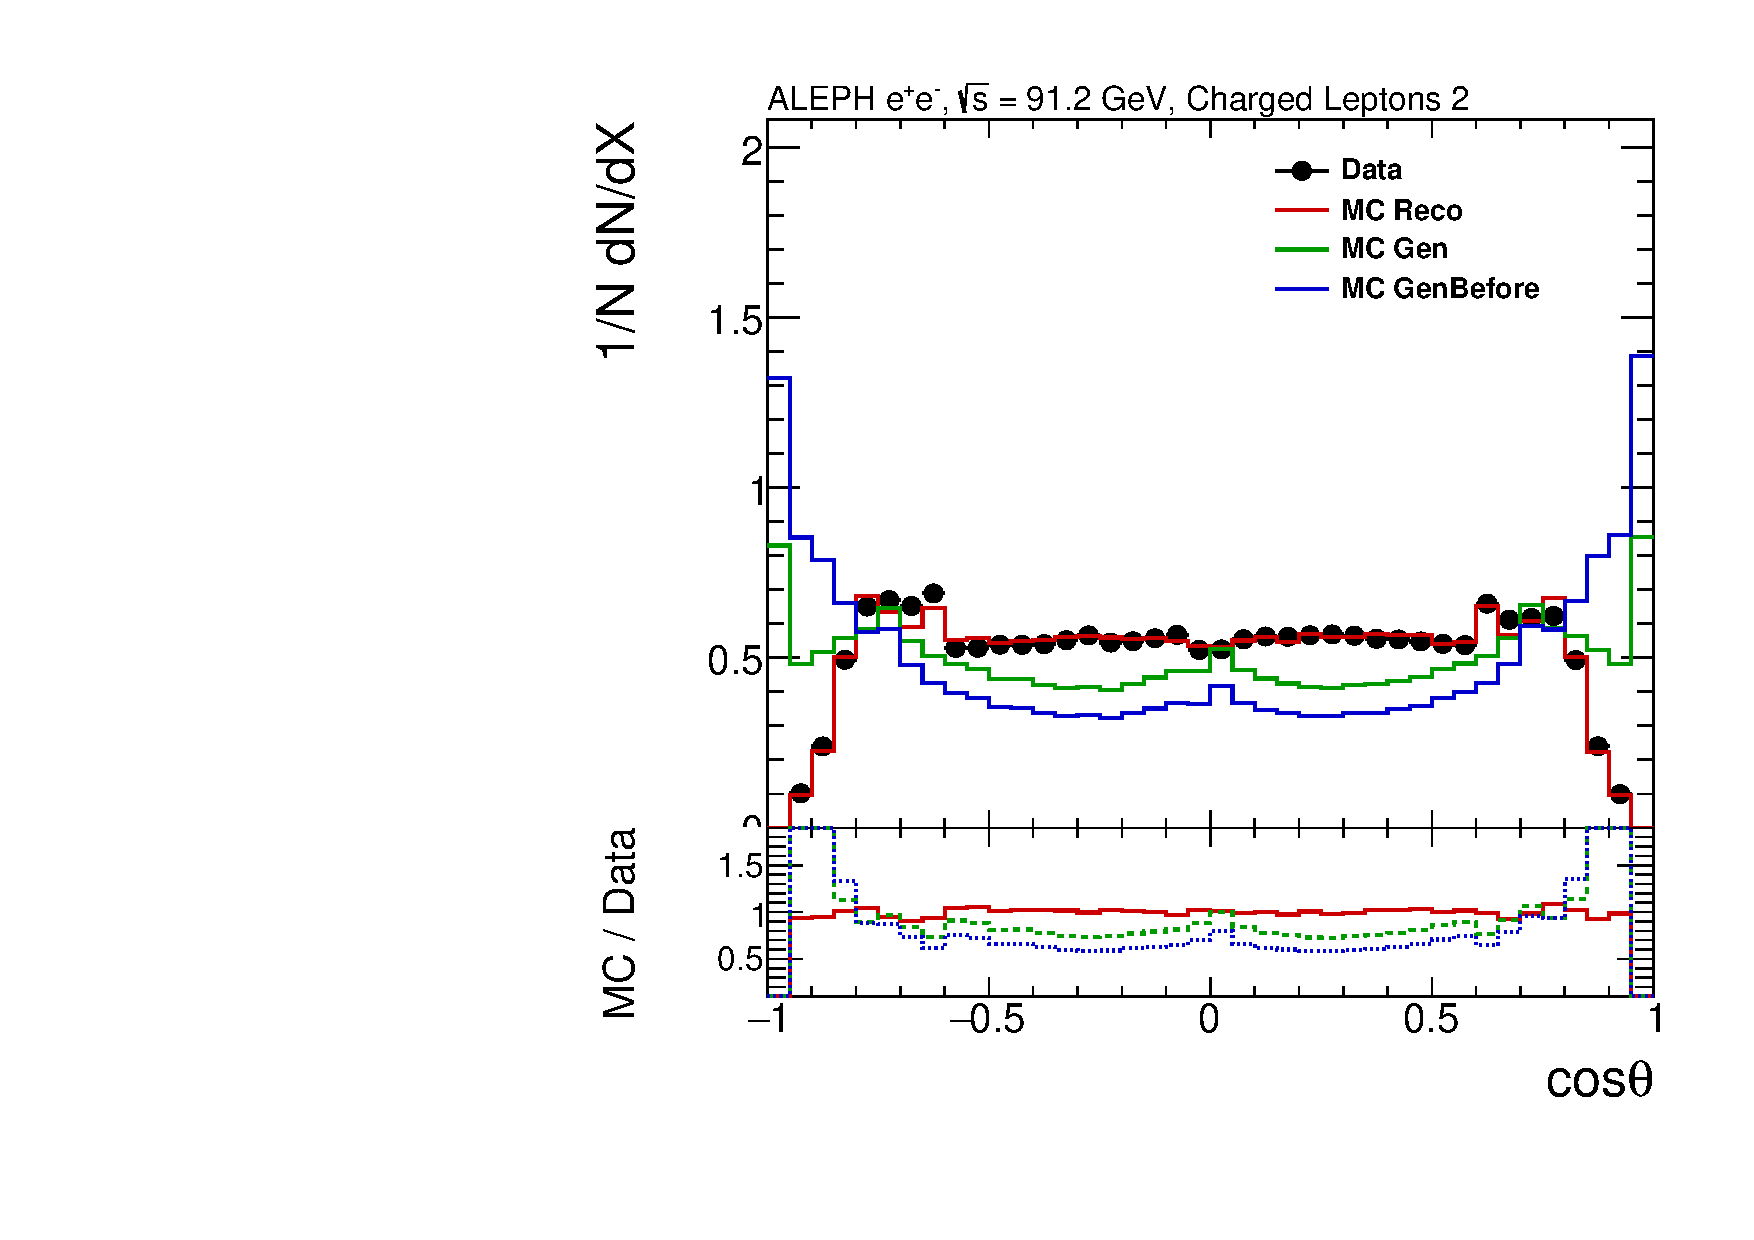
\includegraphics[width=0.242\textwidth]{figures/pwflag2_cosTheta.pdf}
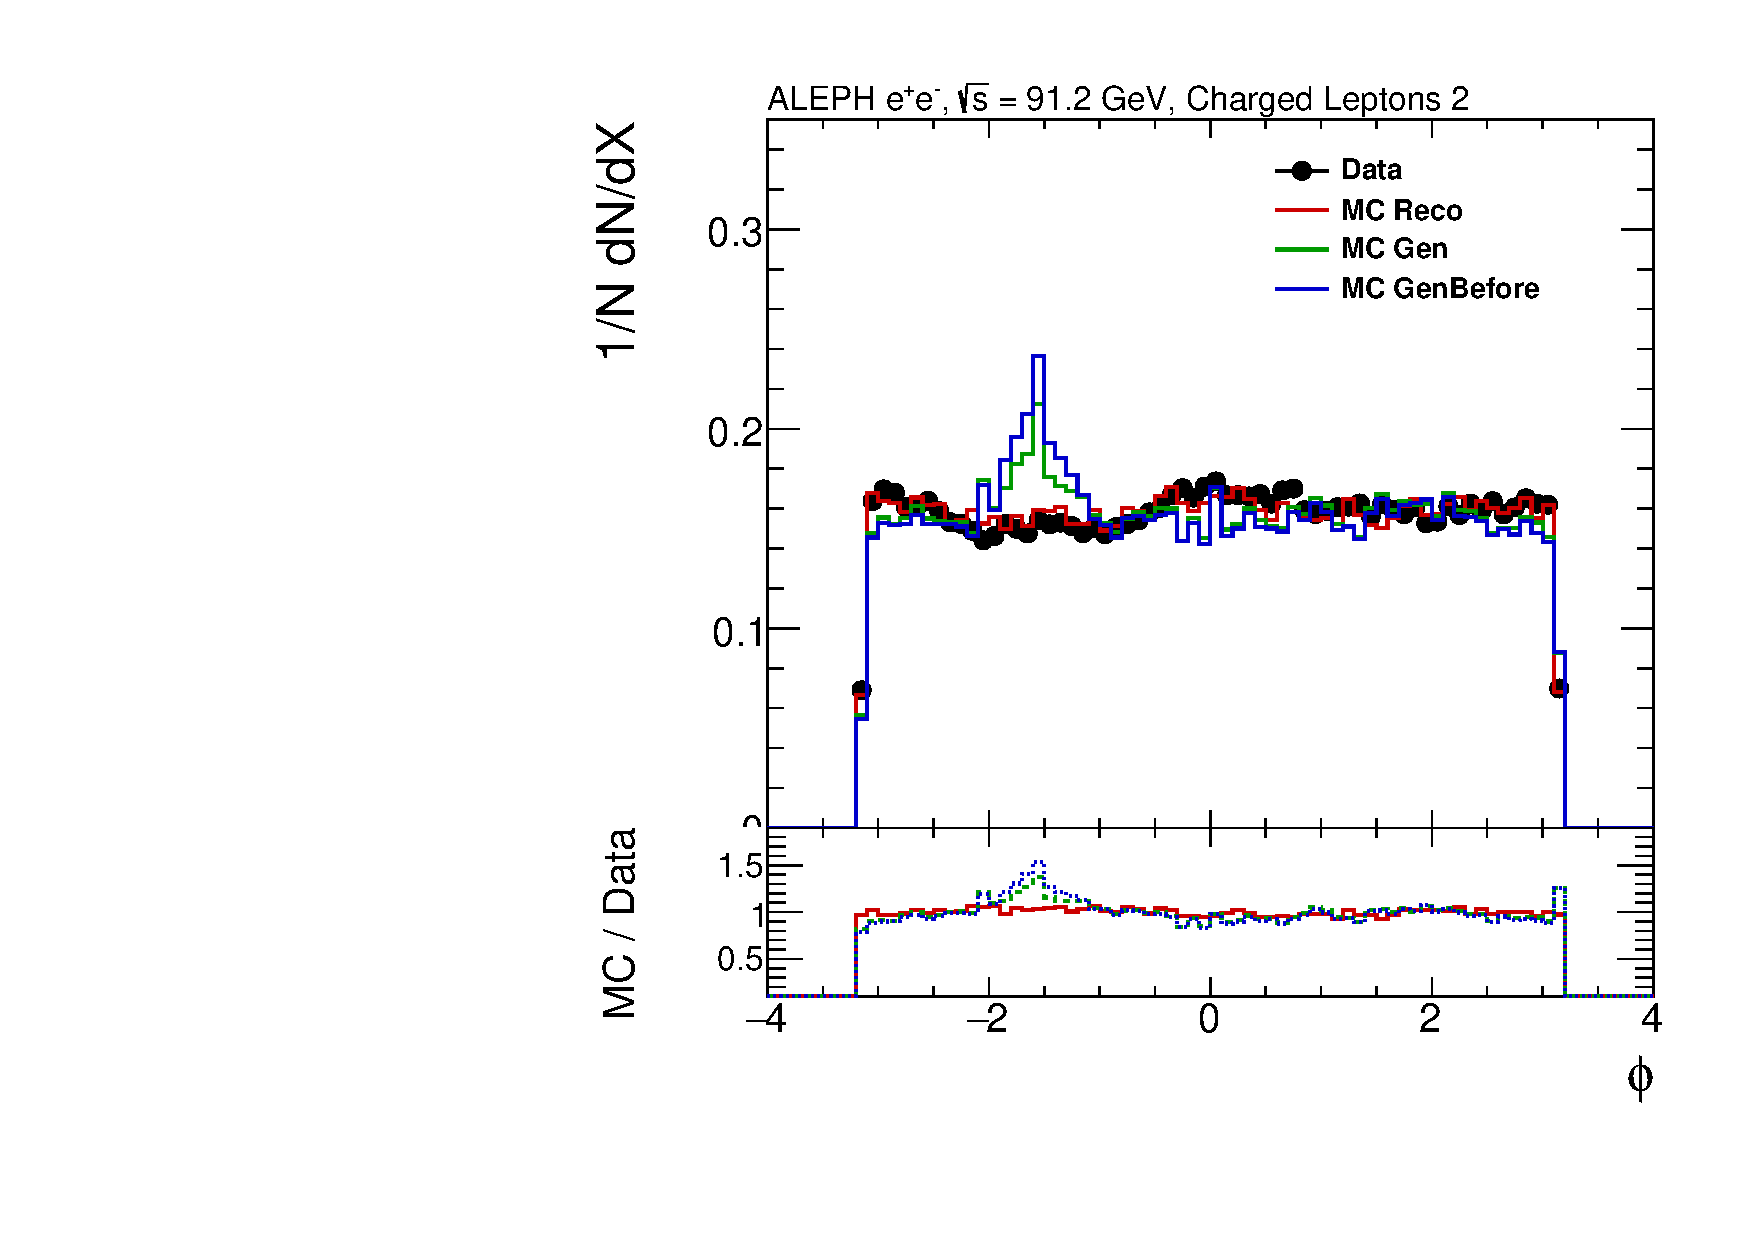
\includegraphics[width=0.242\textwidth]{figures/pwflag2_phi.pdf}
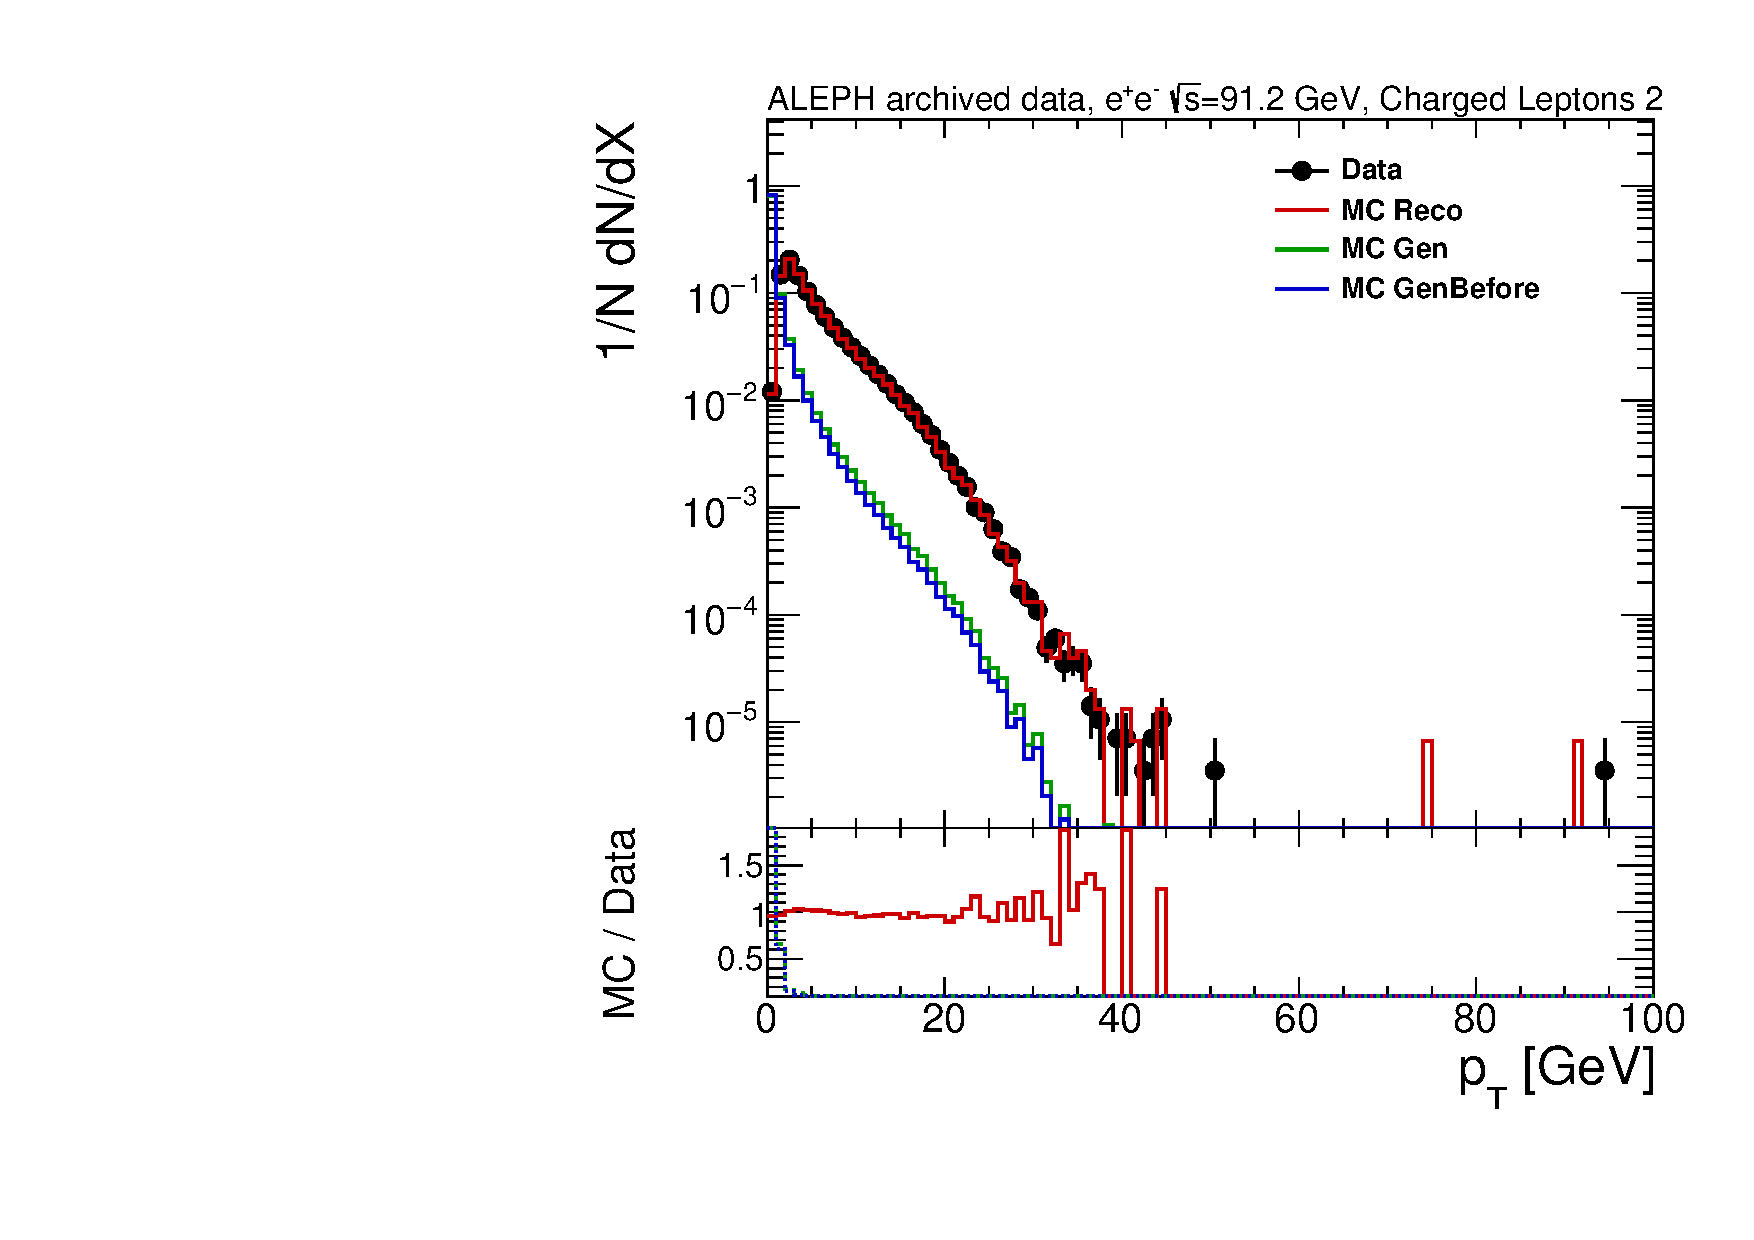
\includegraphics[width=0.242\textwidth]{figures/pwflag2_pt.pdf}
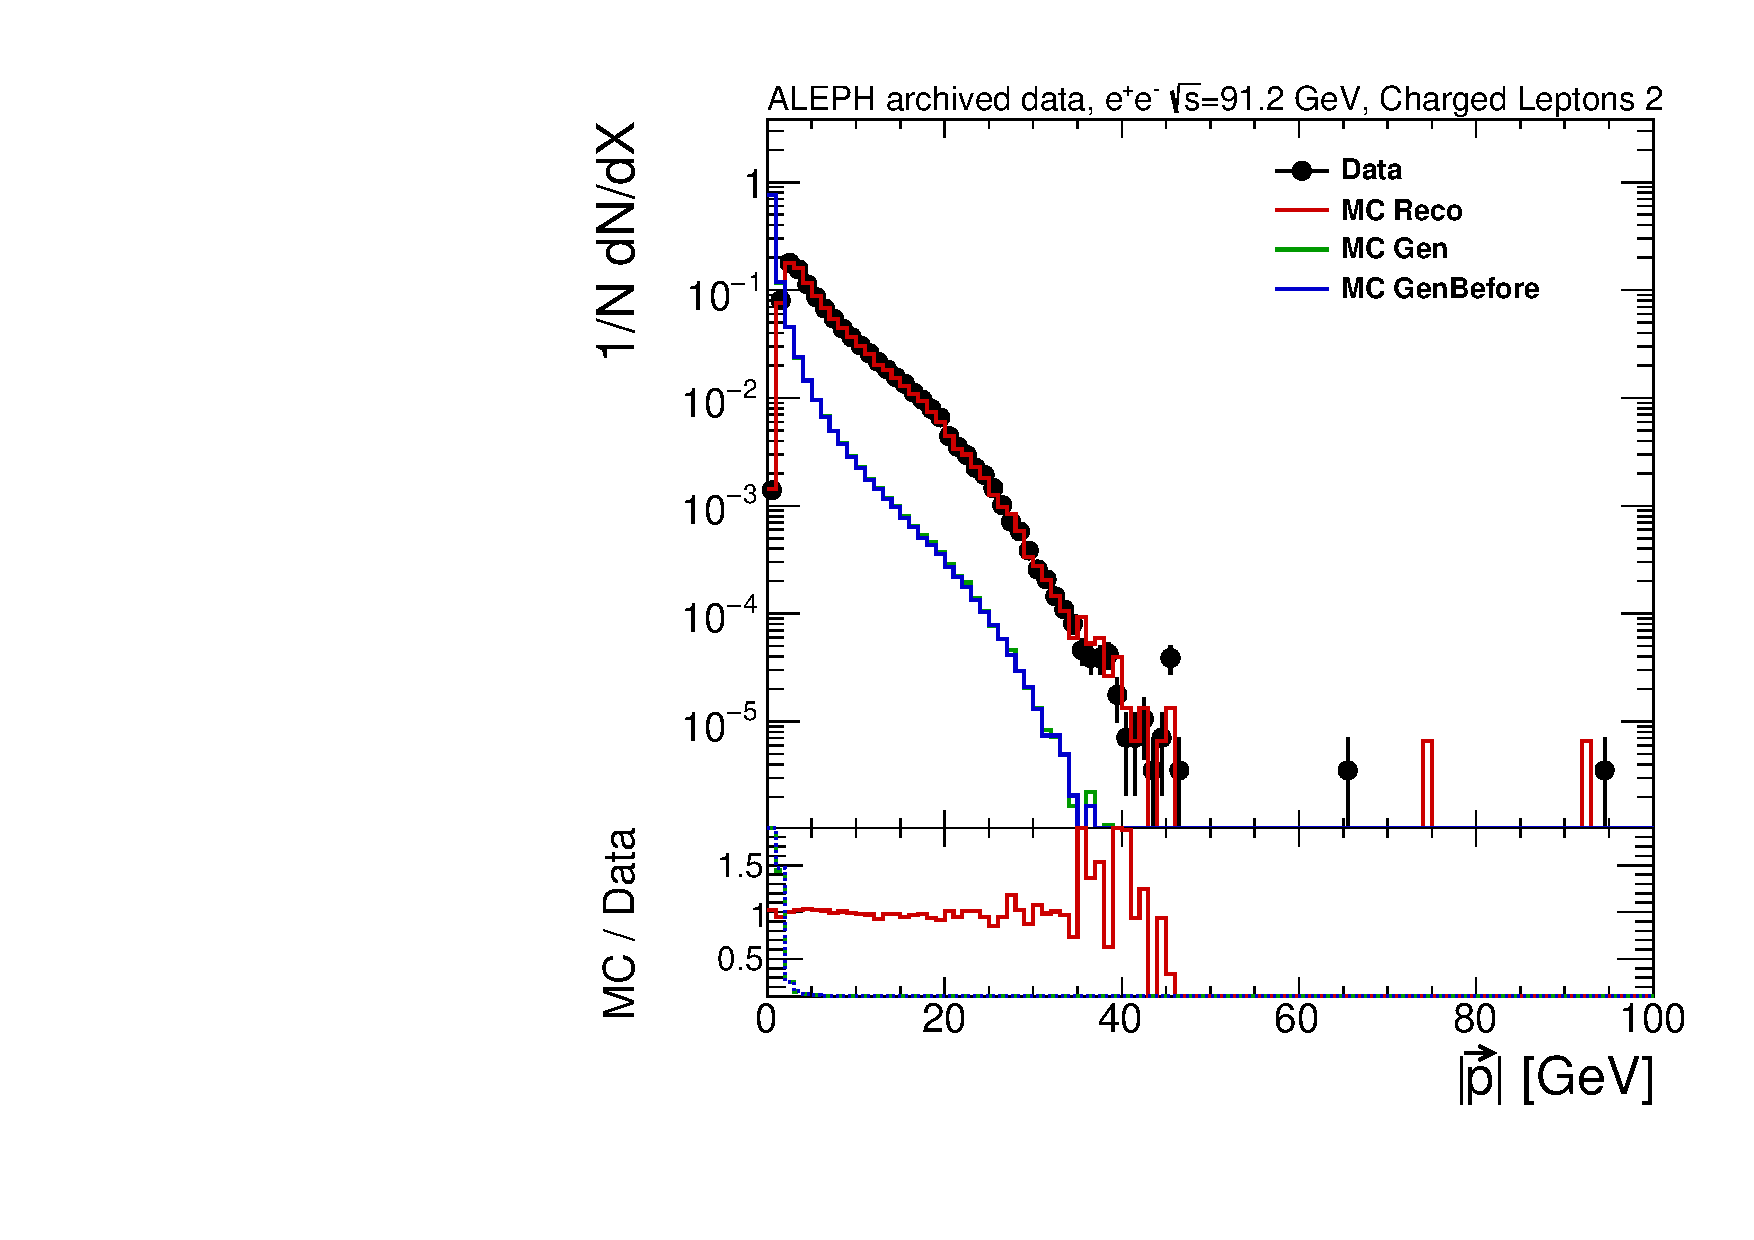
\includegraphics[width=0.242\textwidth]{figures/pwflag2_pmag.pdf}
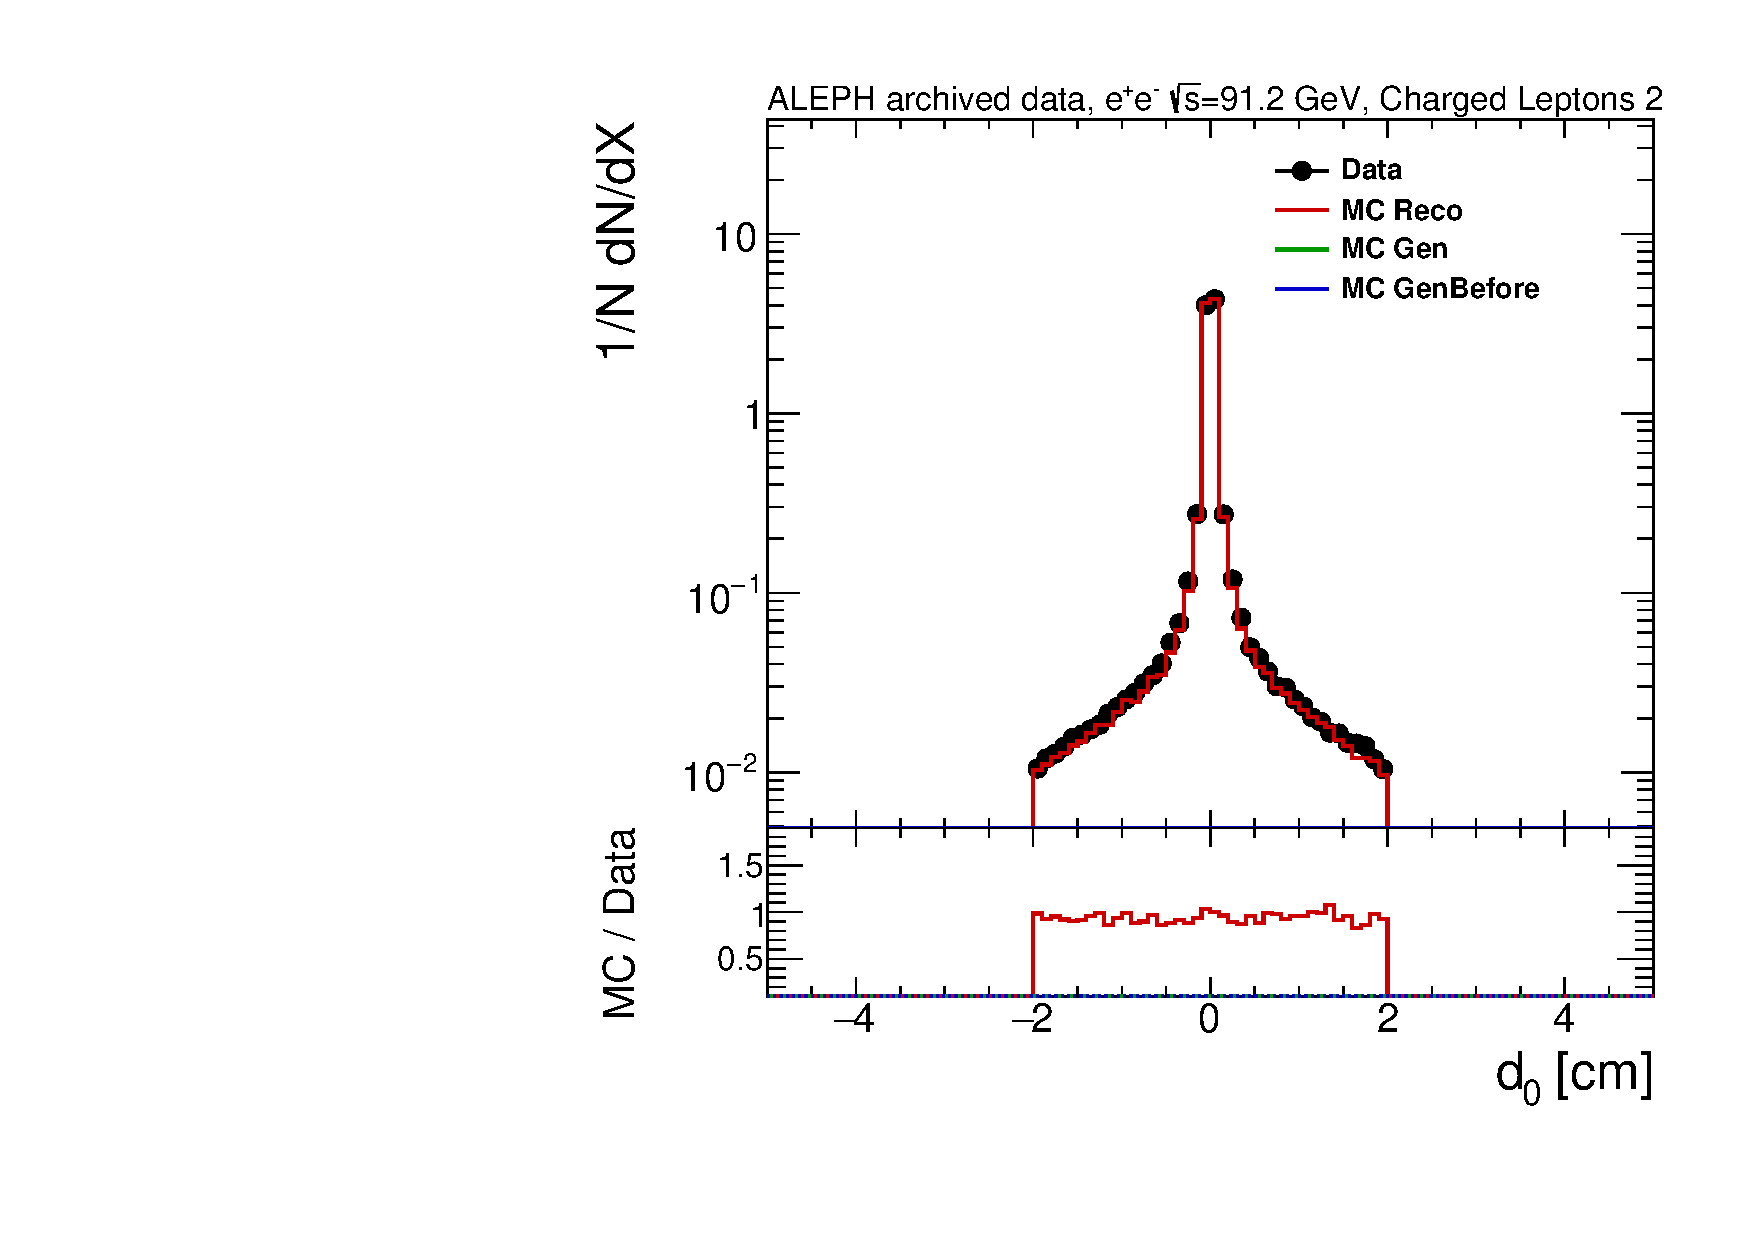
\includegraphics[width=0.242\textwidth]{figures/pwflag2_d0.pdf}
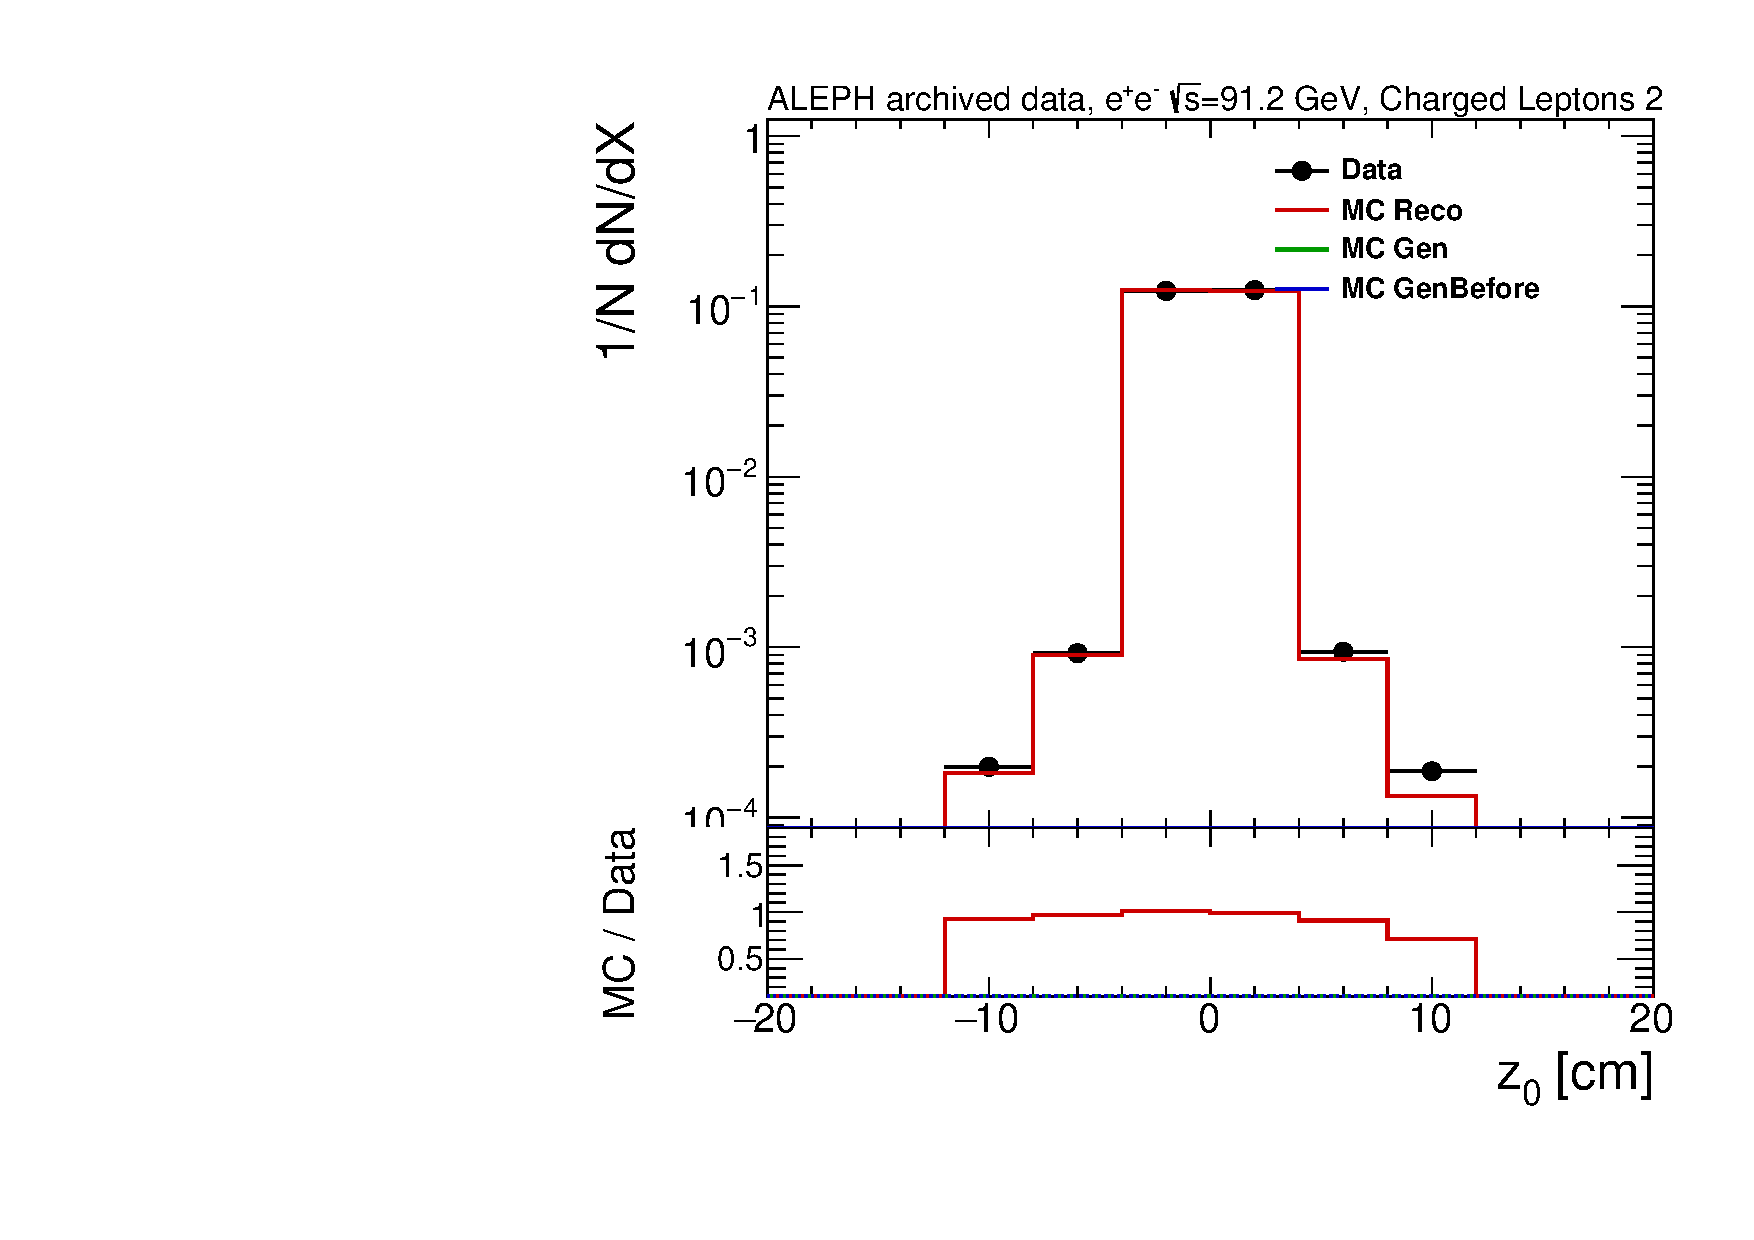
\includegraphics[width=0.242\textwidth]{figures/pwflag2_z0.pdf}
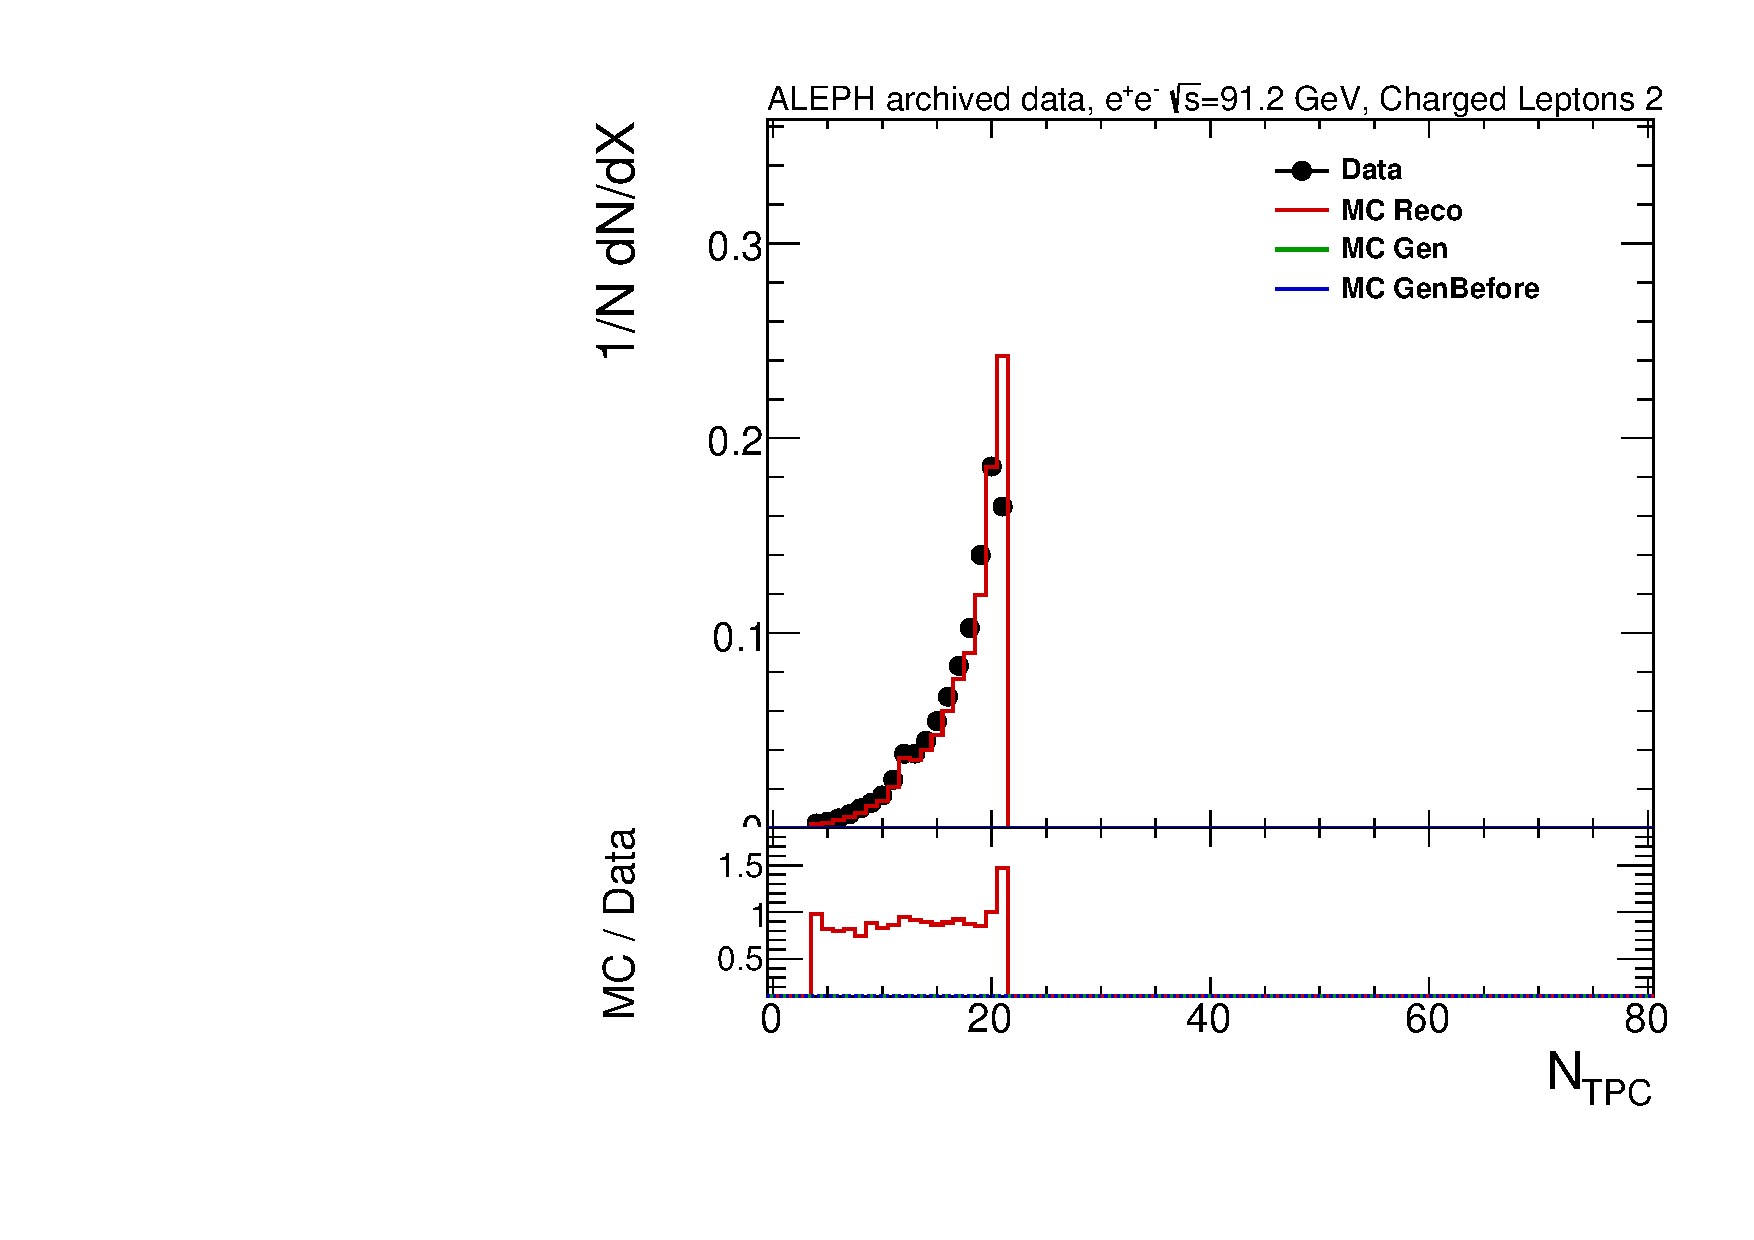
\includegraphics[width=0.242\textwidth]{figures/pwflag2_ntpc.pdf}
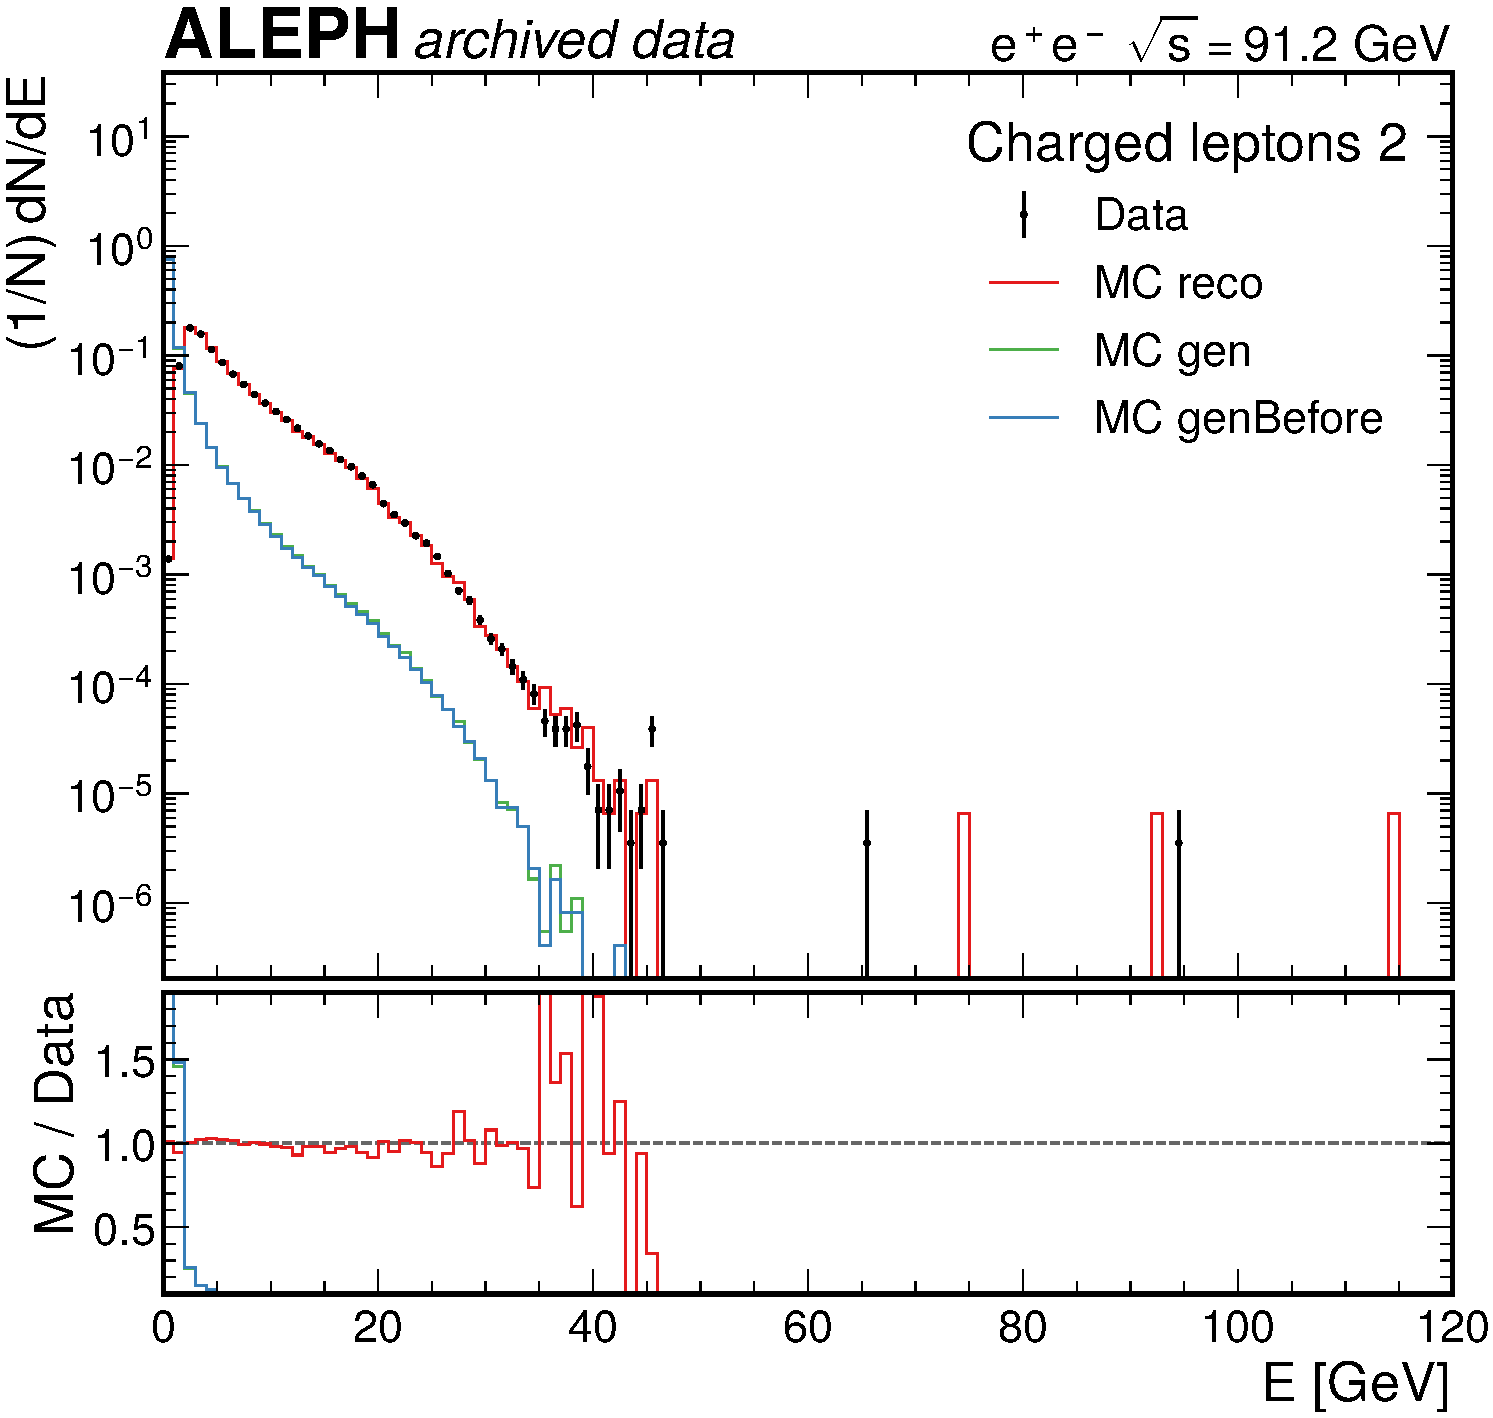
\includegraphics[width=0.242\textwidth]{figures/pwflag2_energy.pdf}
% 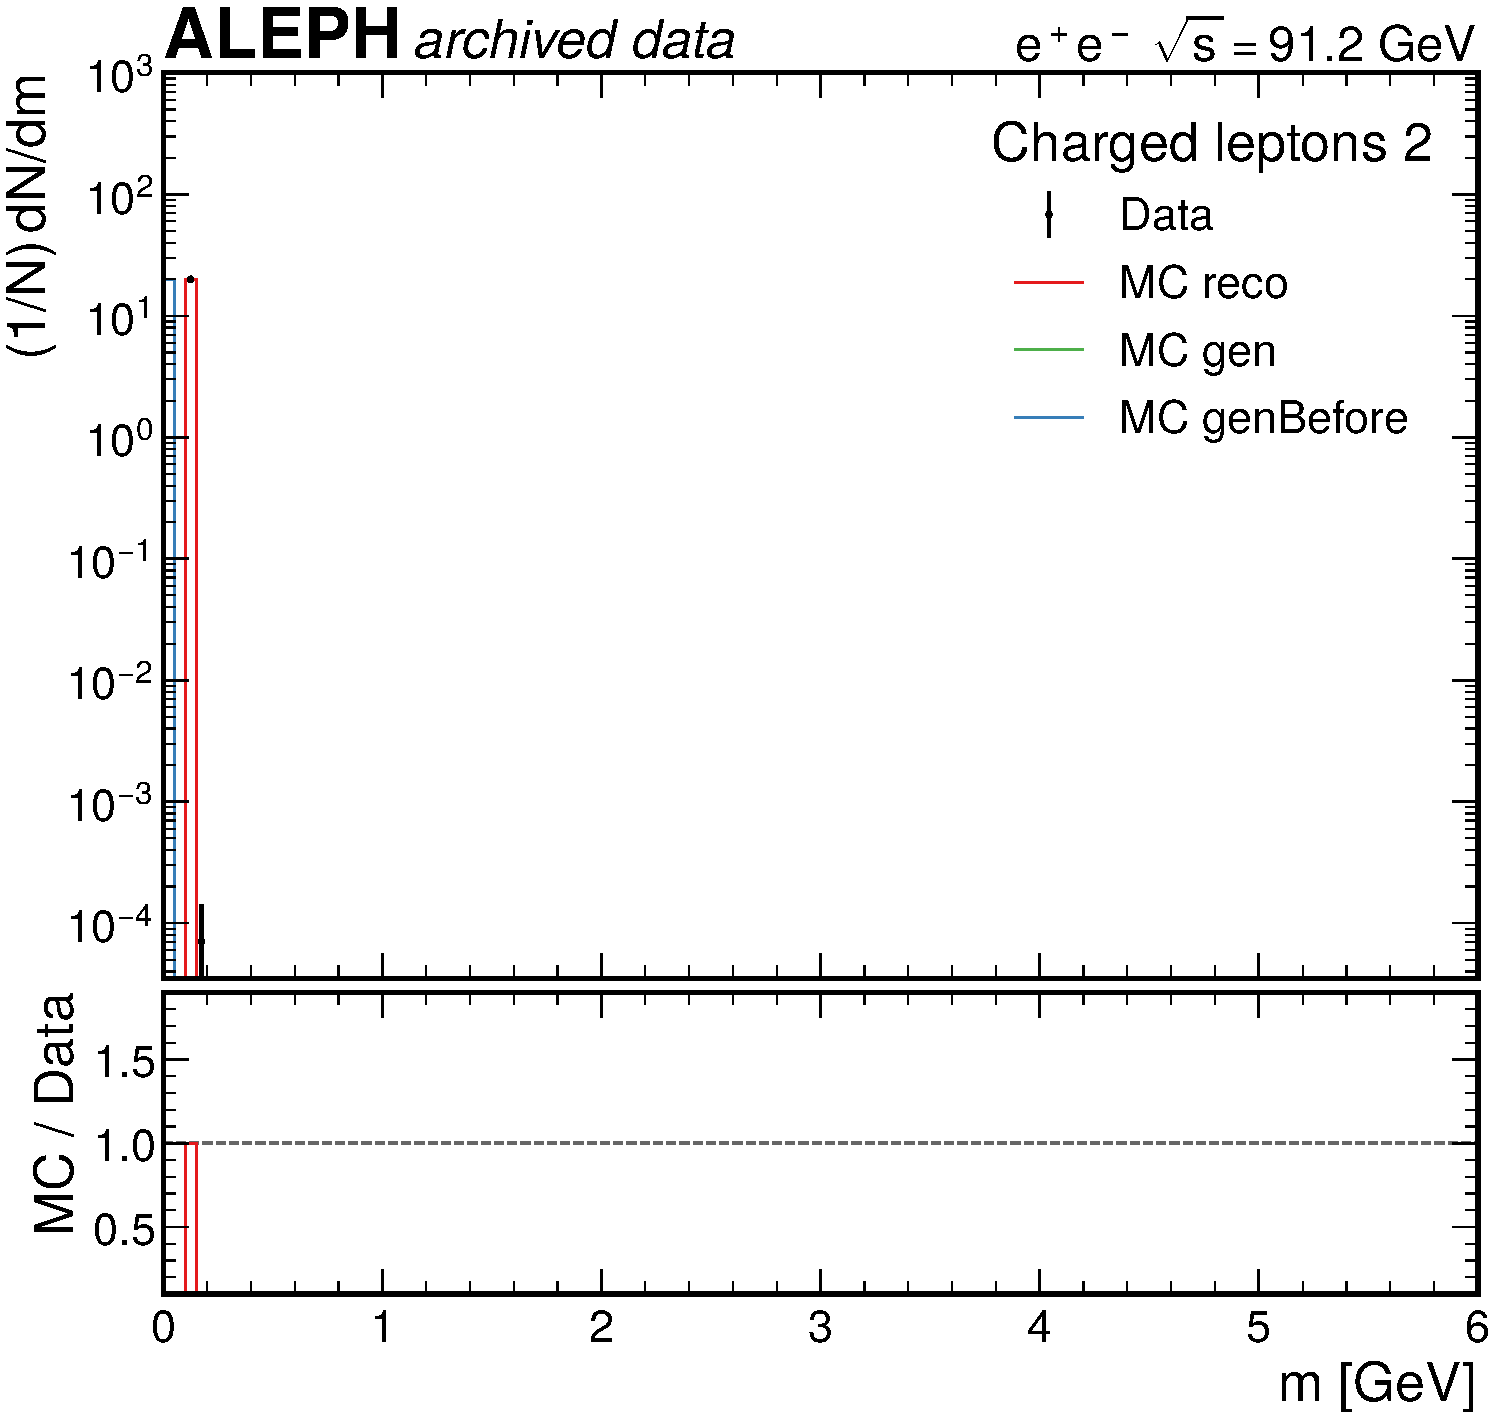
\includegraphics[width=0.242\textwidth]{figures/pwflag2_mass.pdf}
\caption{Complete \texttt{pwflag}=2 kinematic set.}
\label{fig:pwflag2_full}
\end{figure}

\begin{figure}[t!]
\centering
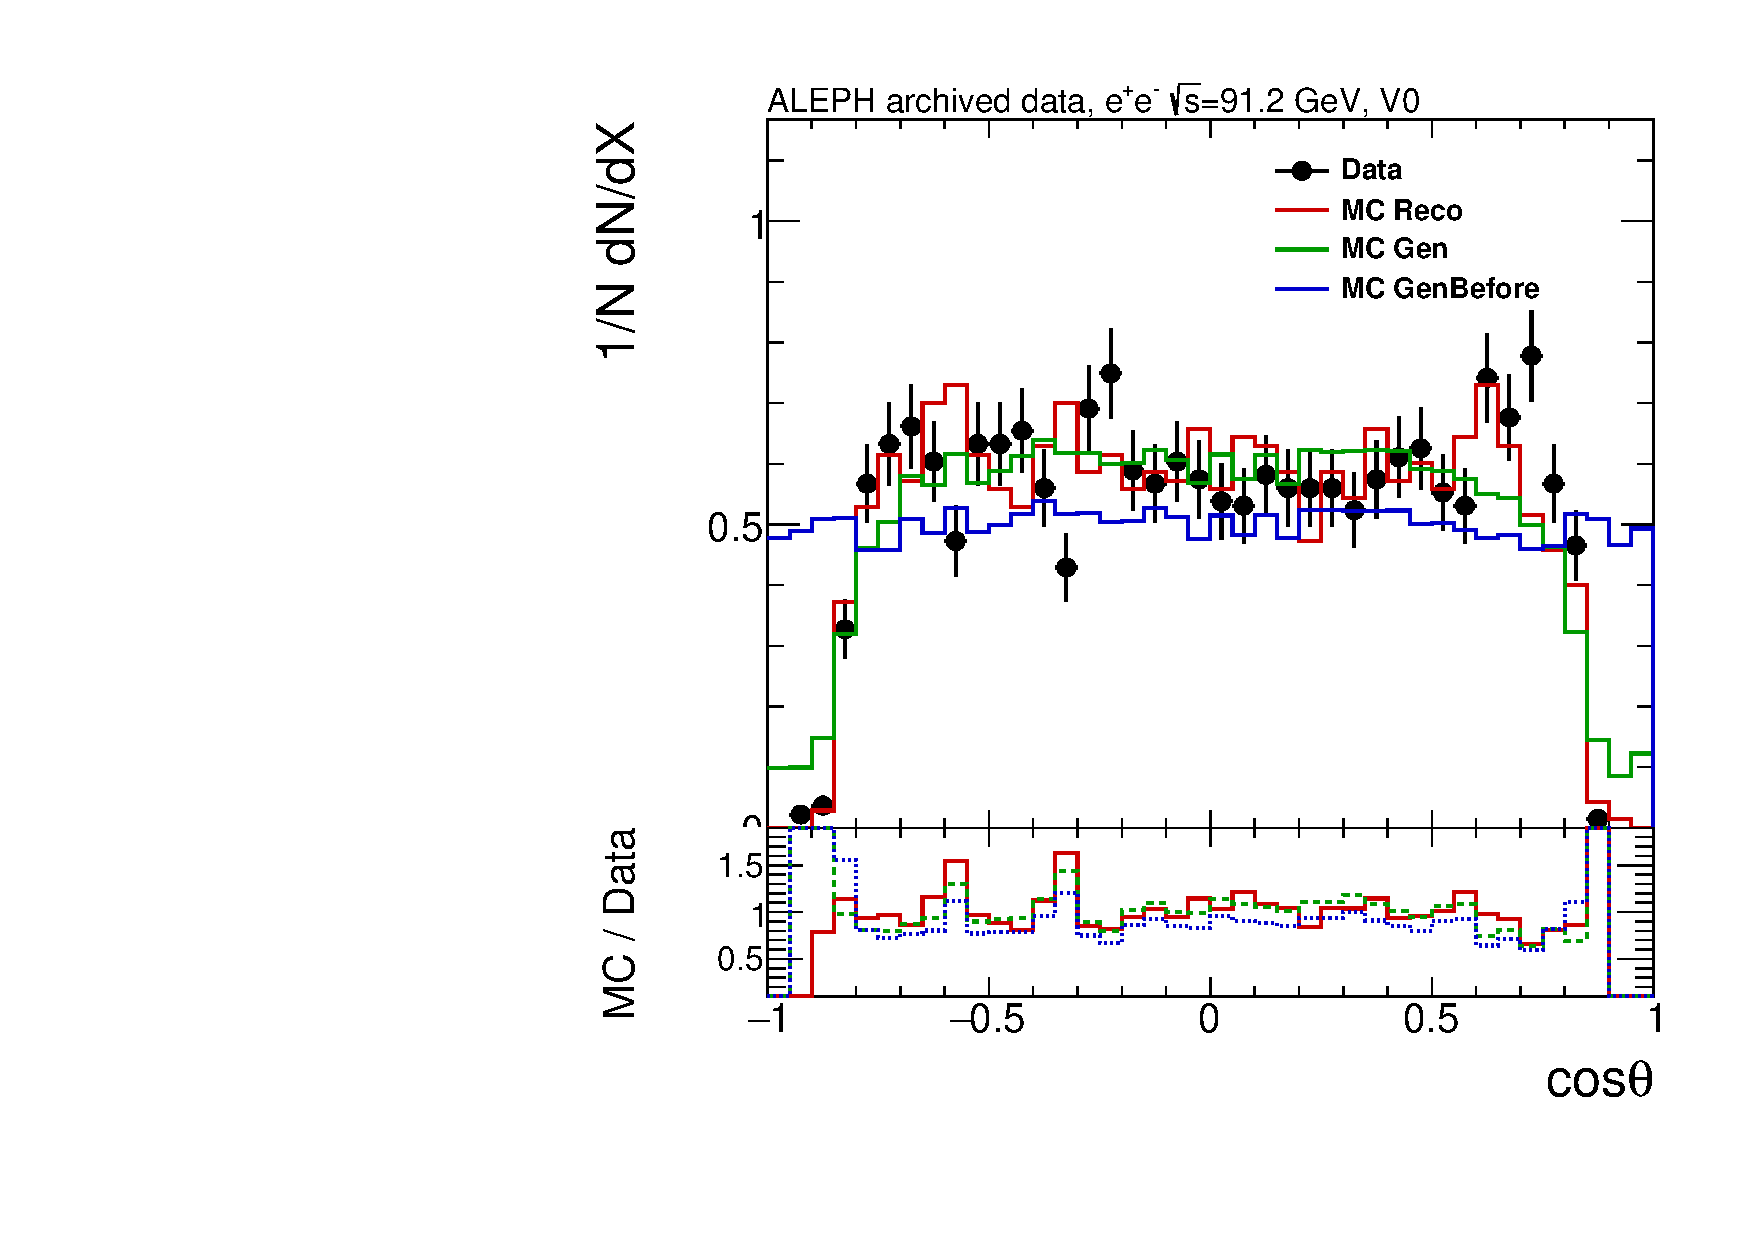
\includegraphics[width=0.495\textwidth]{figures/pwflag3_cosTheta.pdf}
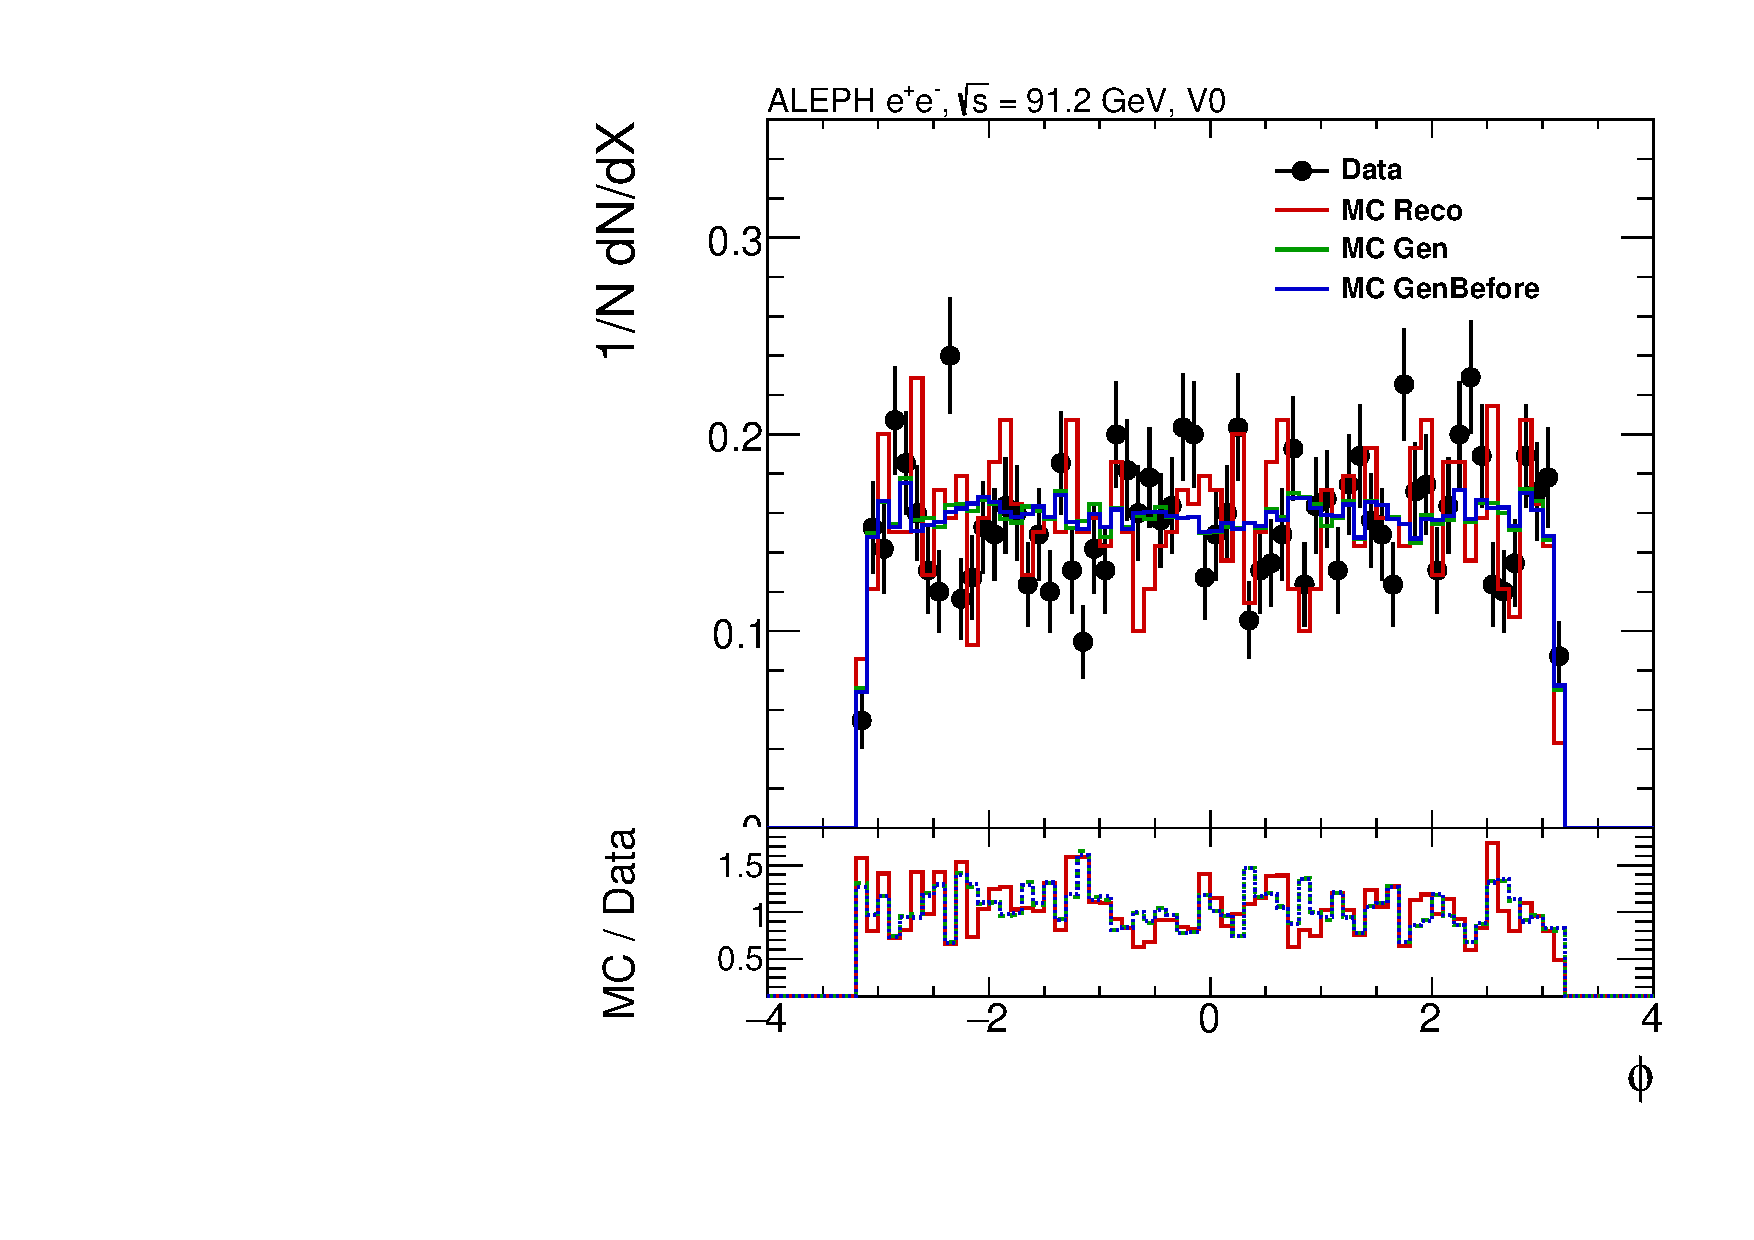
\includegraphics[width=0.495\textwidth]{figures/pwflag3_phi.pdf}
% 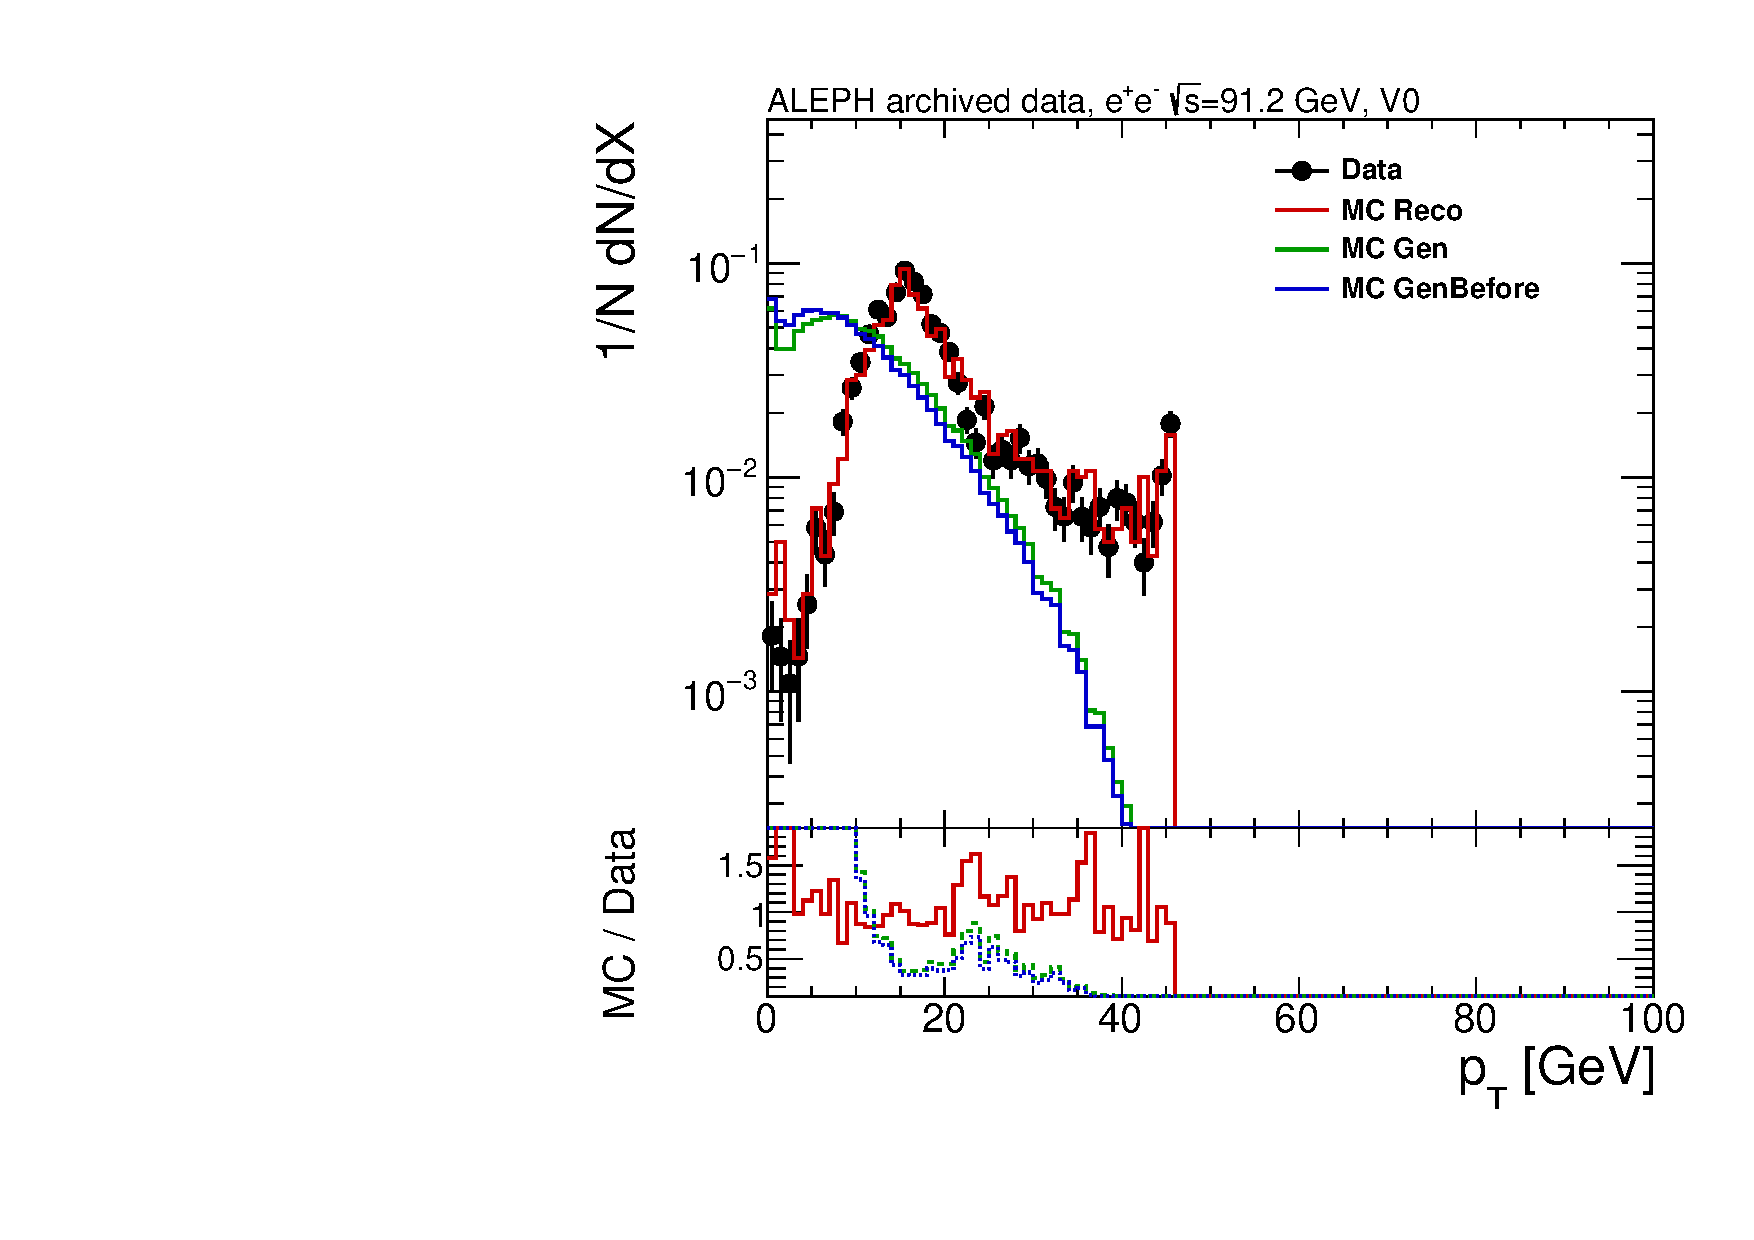
\includegraphics[width=0.242\textwidth]{figures/pwflag3_pt.pdf}
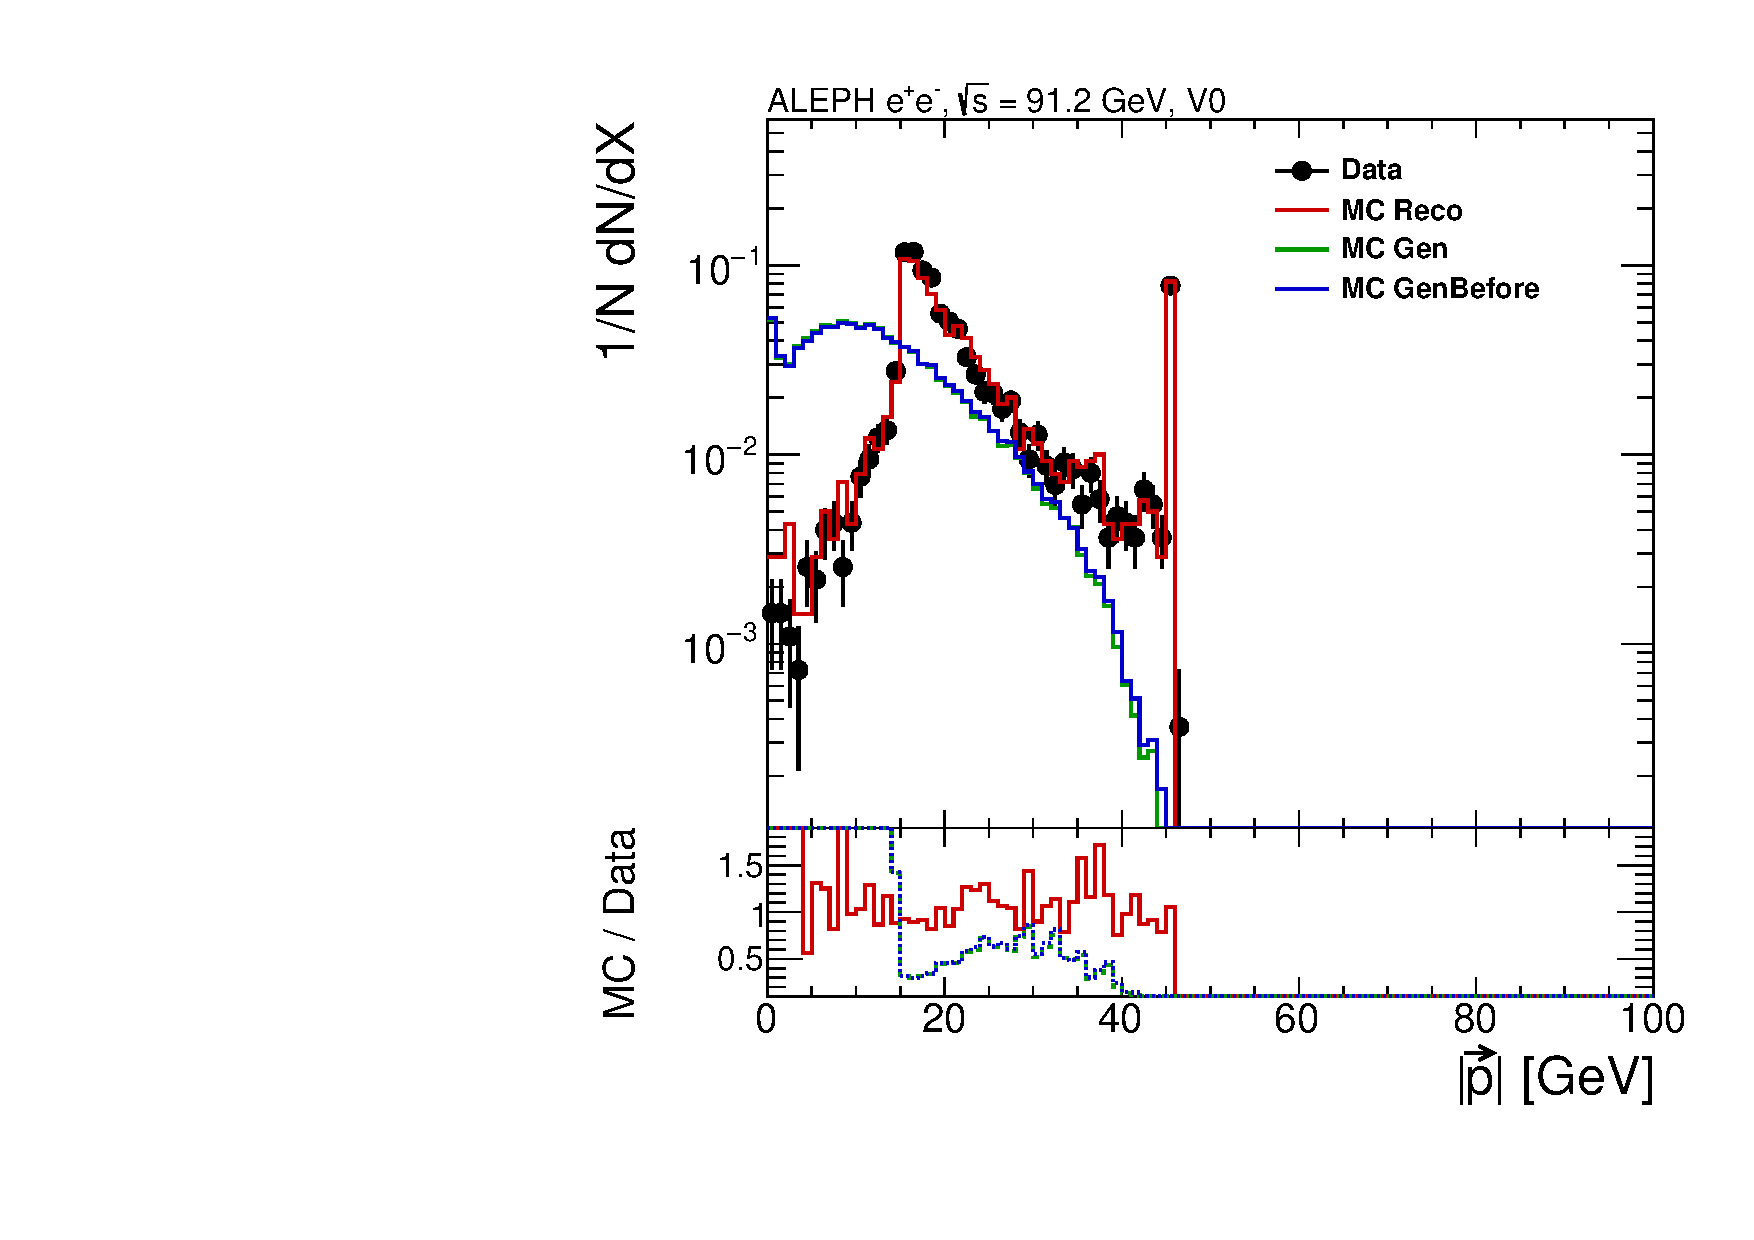
\includegraphics[width=0.495\textwidth]{figures/pwflag3_pmag.pdf}
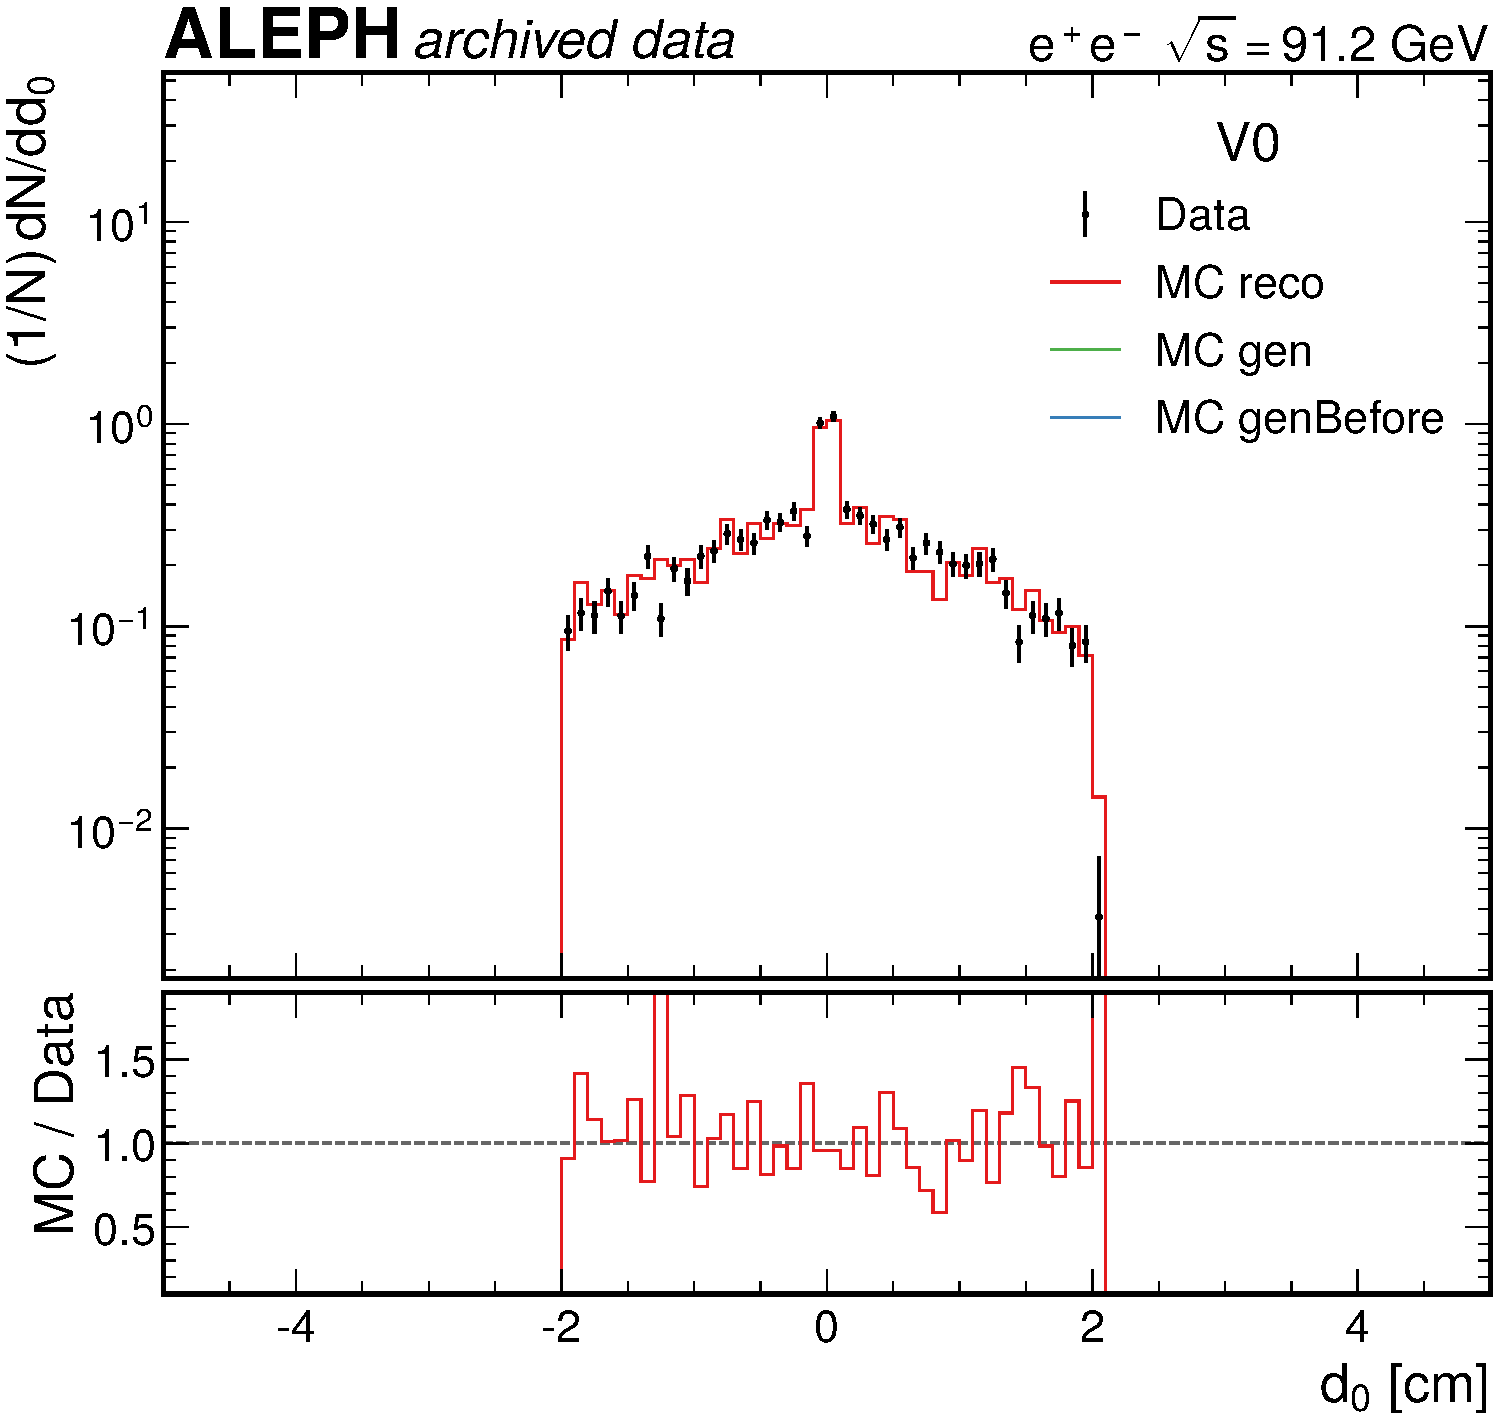
\includegraphics[width=0.495\textwidth]{figures/pwflag3_d0.pdf}
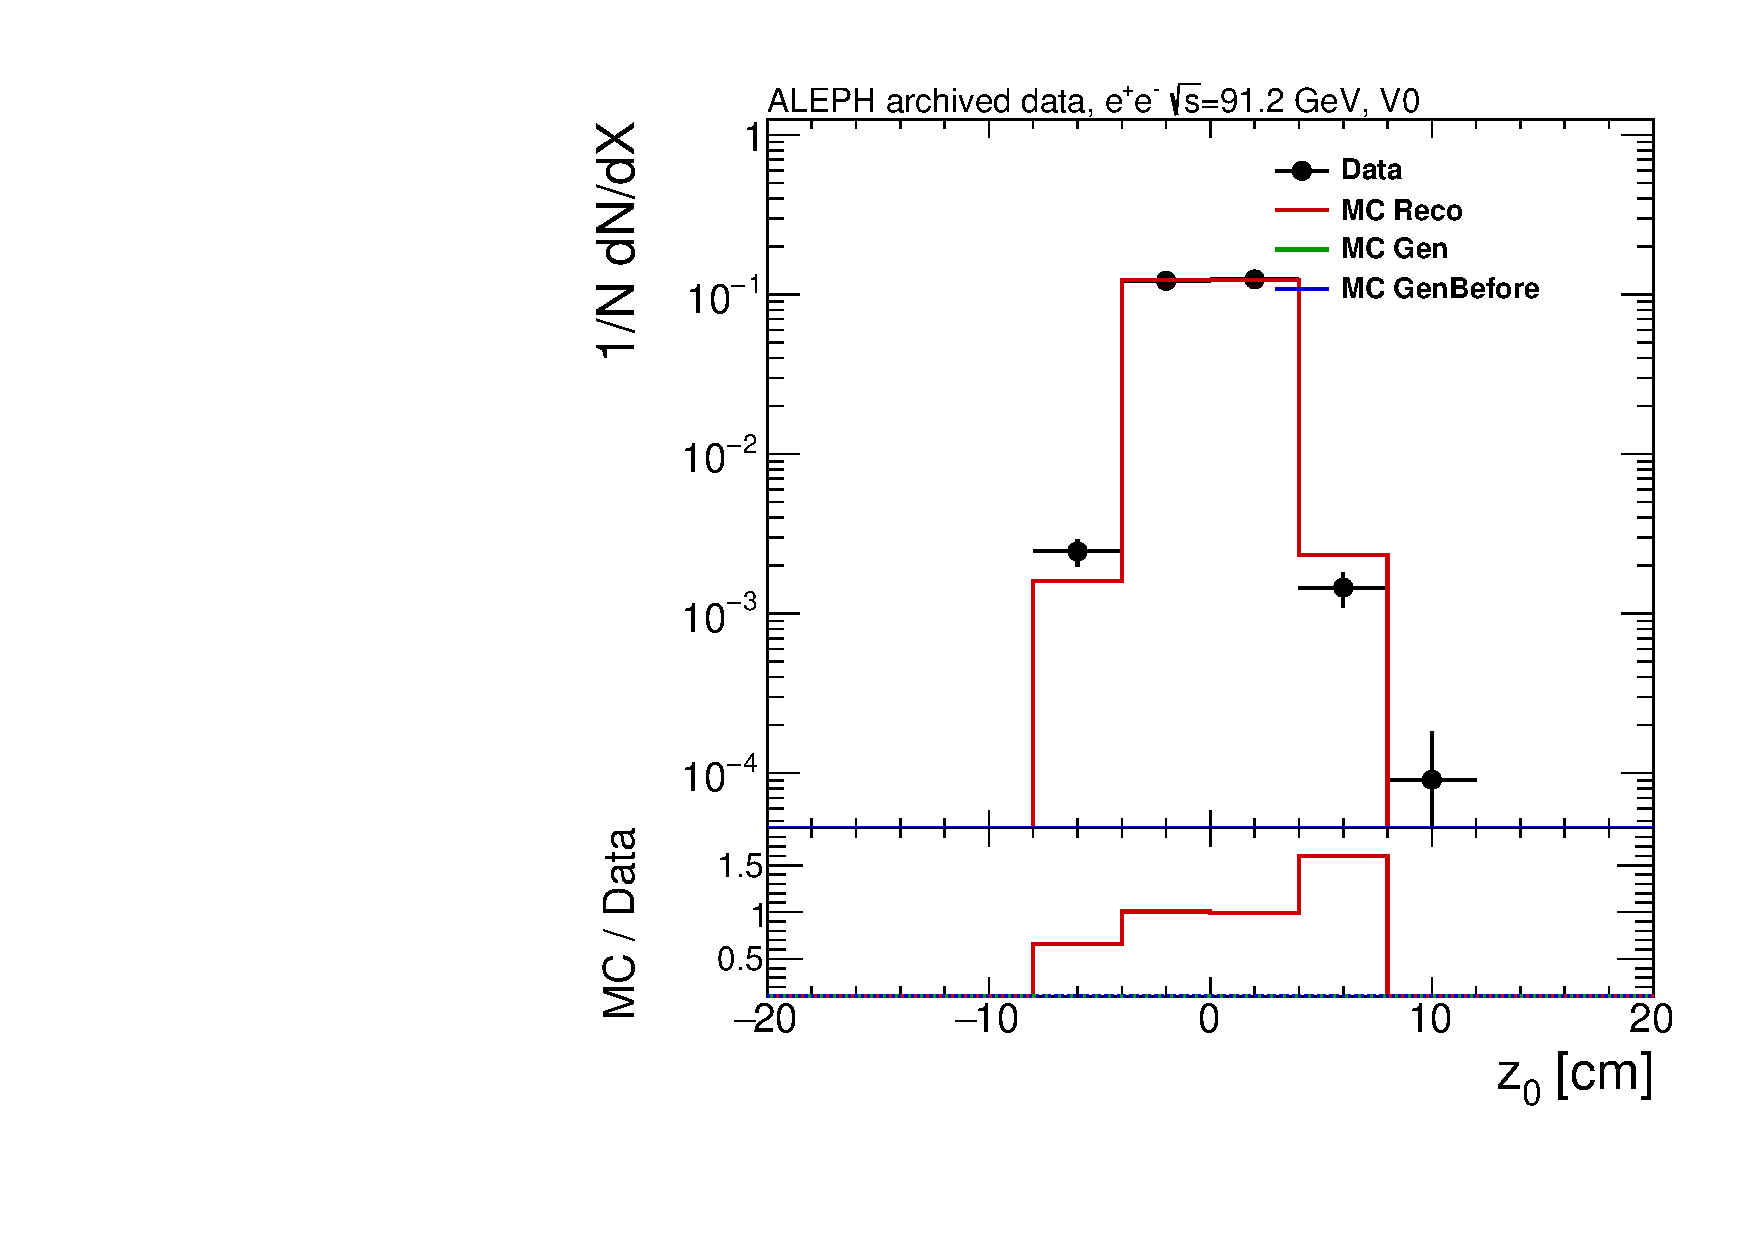
\includegraphics[width=0.495\textwidth]{figures/pwflag3_z0.pdf}
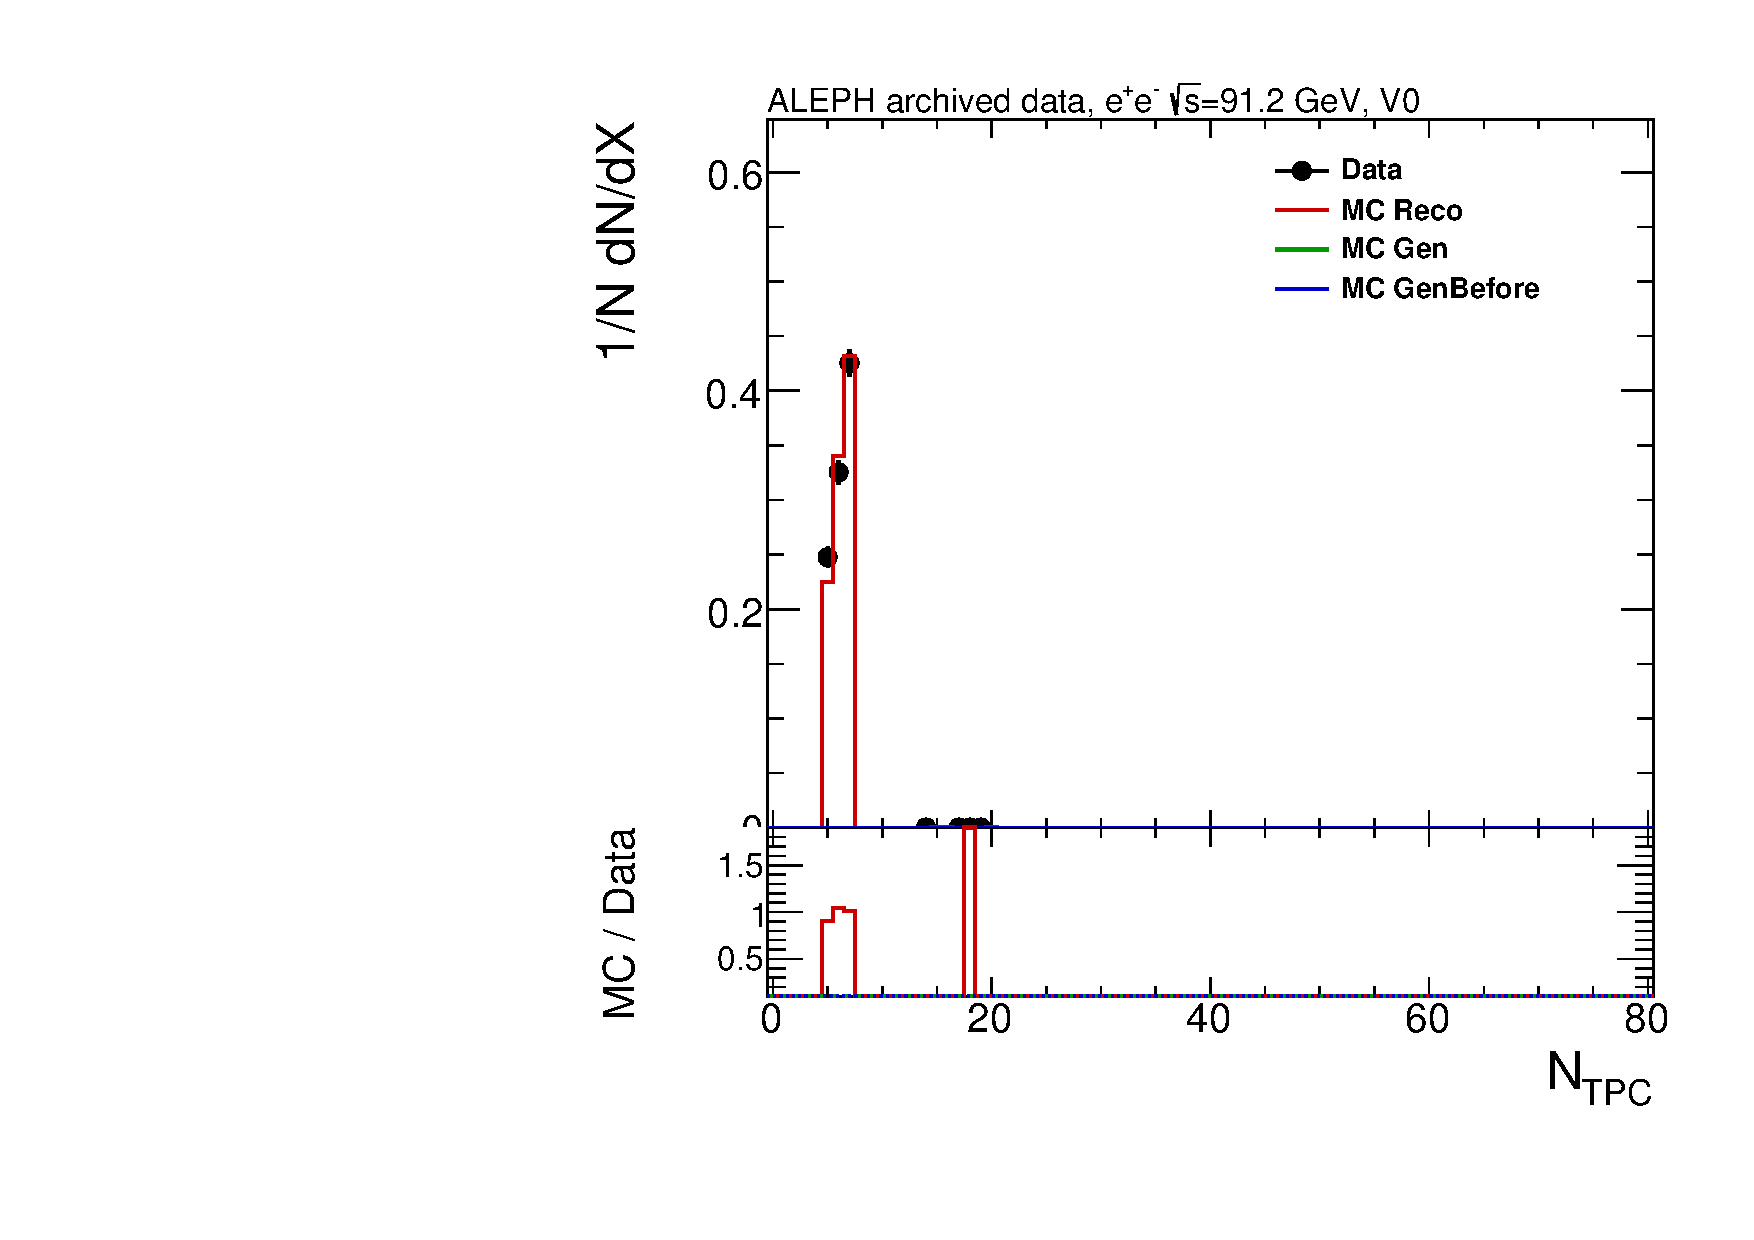
\includegraphics[width=0.495\textwidth]{figures/pwflag3_ntpc.pdf}
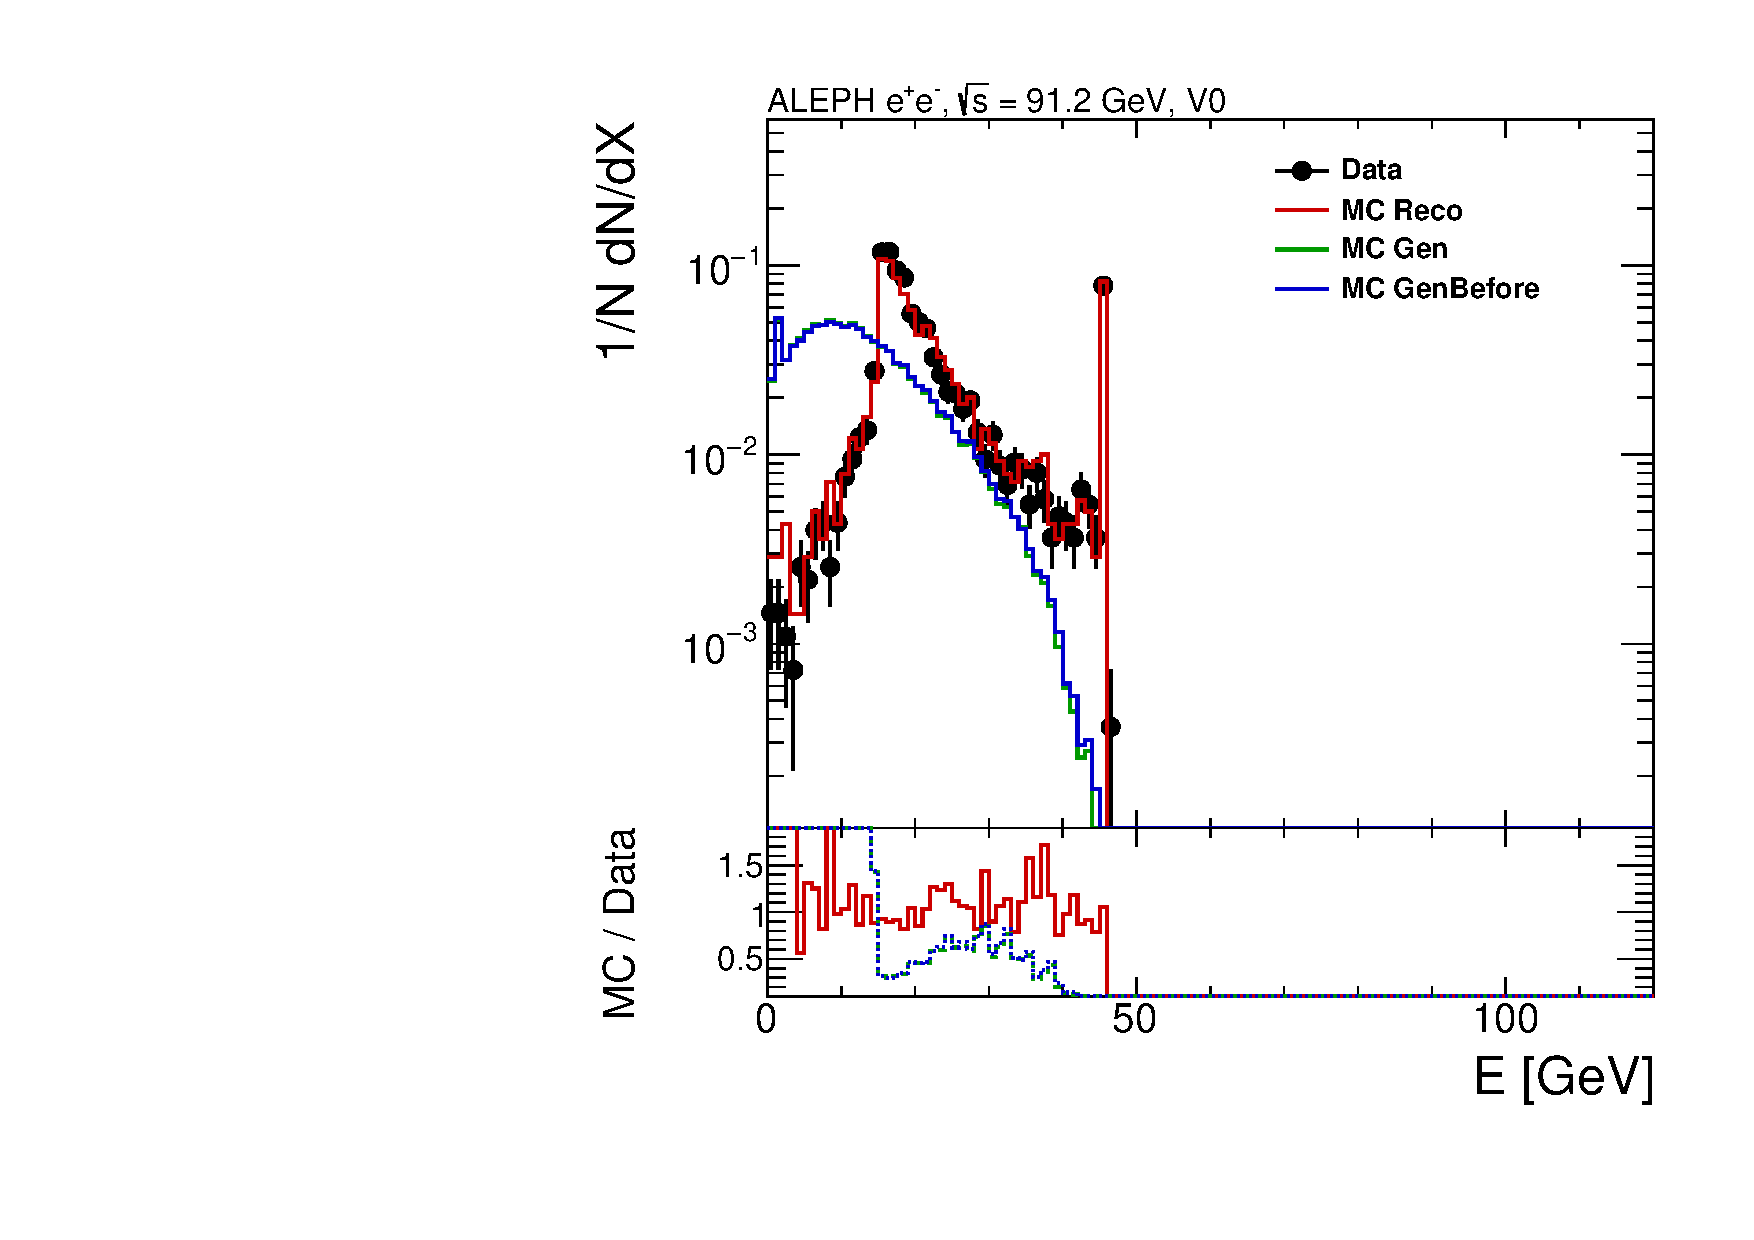
\includegraphics[width=0.495\textwidth]{figures/pwflag3_energy.pdf}
% 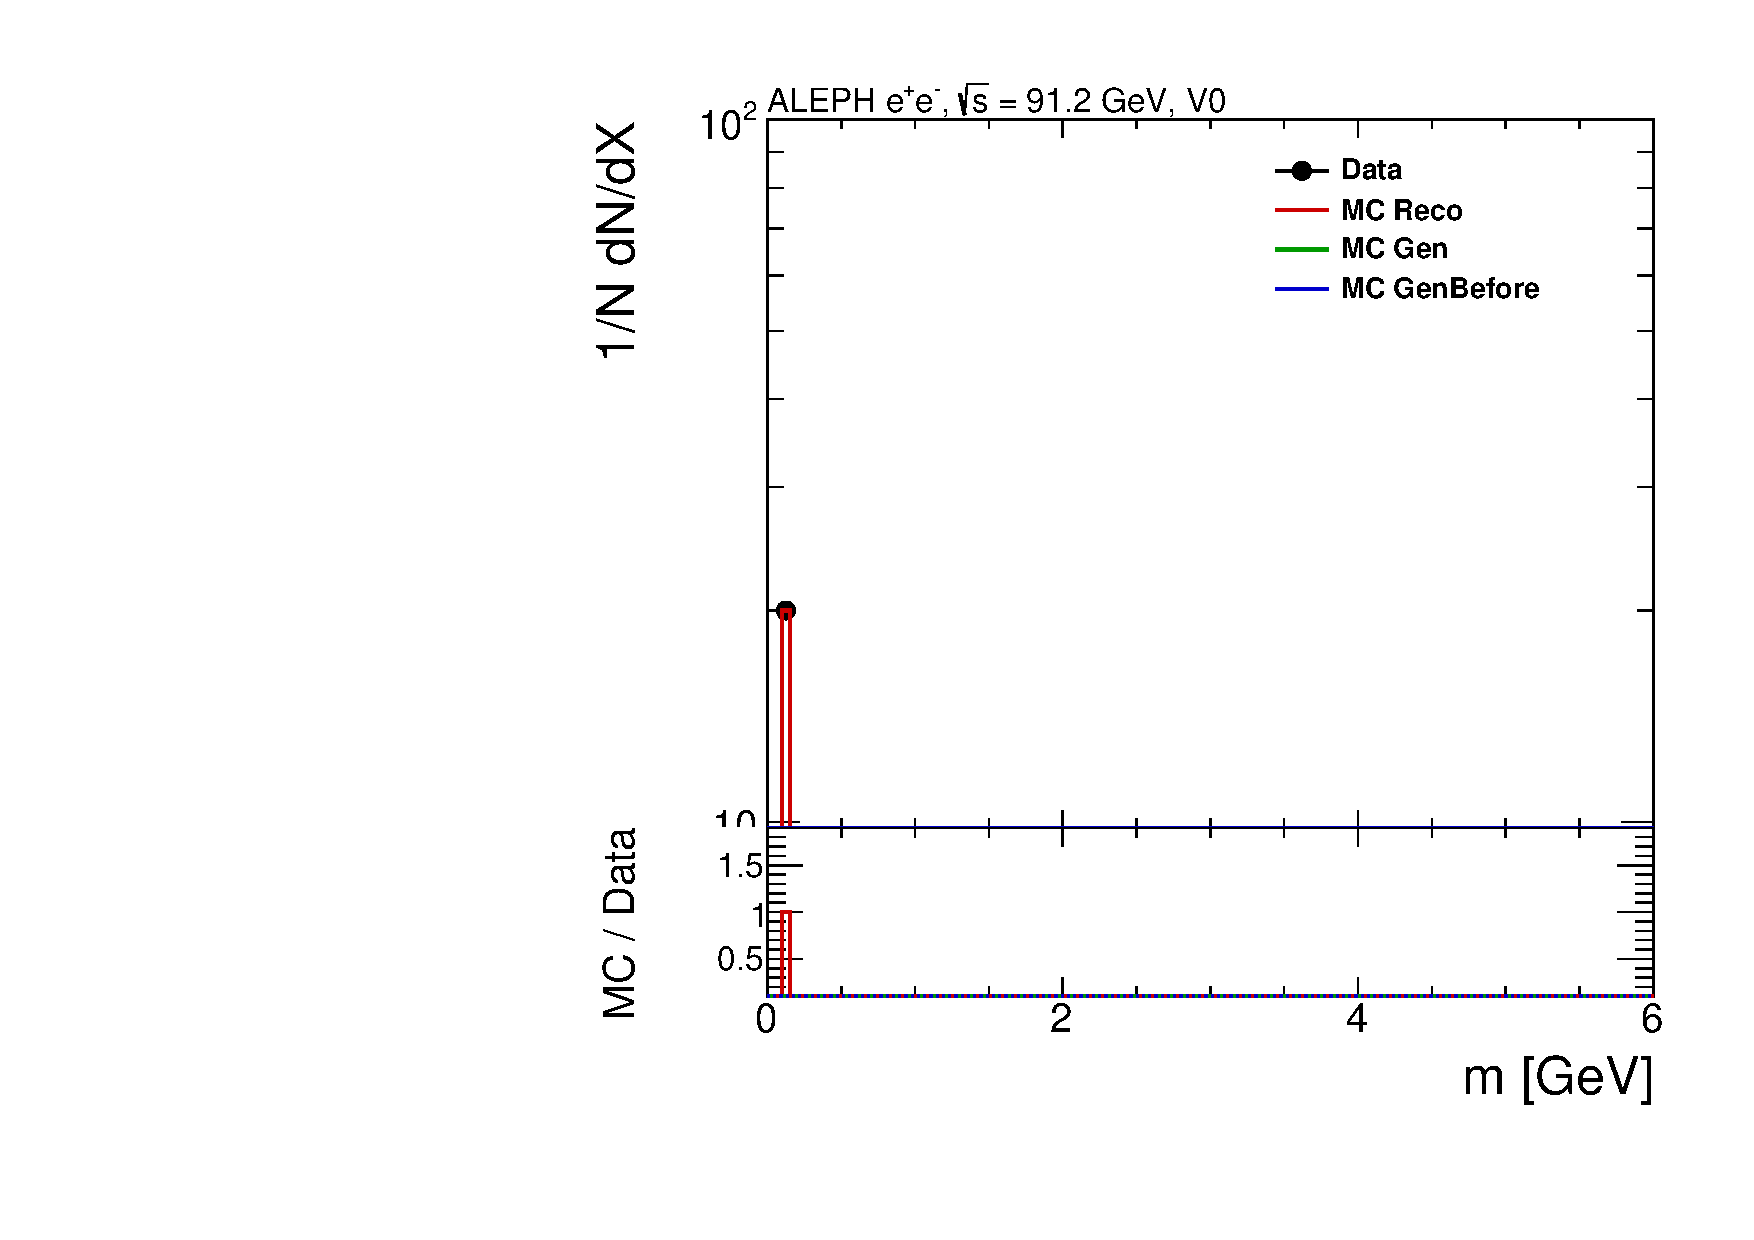
\includegraphics[width=0.242\textwidth]{figures/pwflag3_mass.pdf}
\caption{Complete \texttt{pwflag}=3 kinematic set.}
\label{fig:pwflag3_full}
\end{figure}

\begin{figure}[t!]
\centering
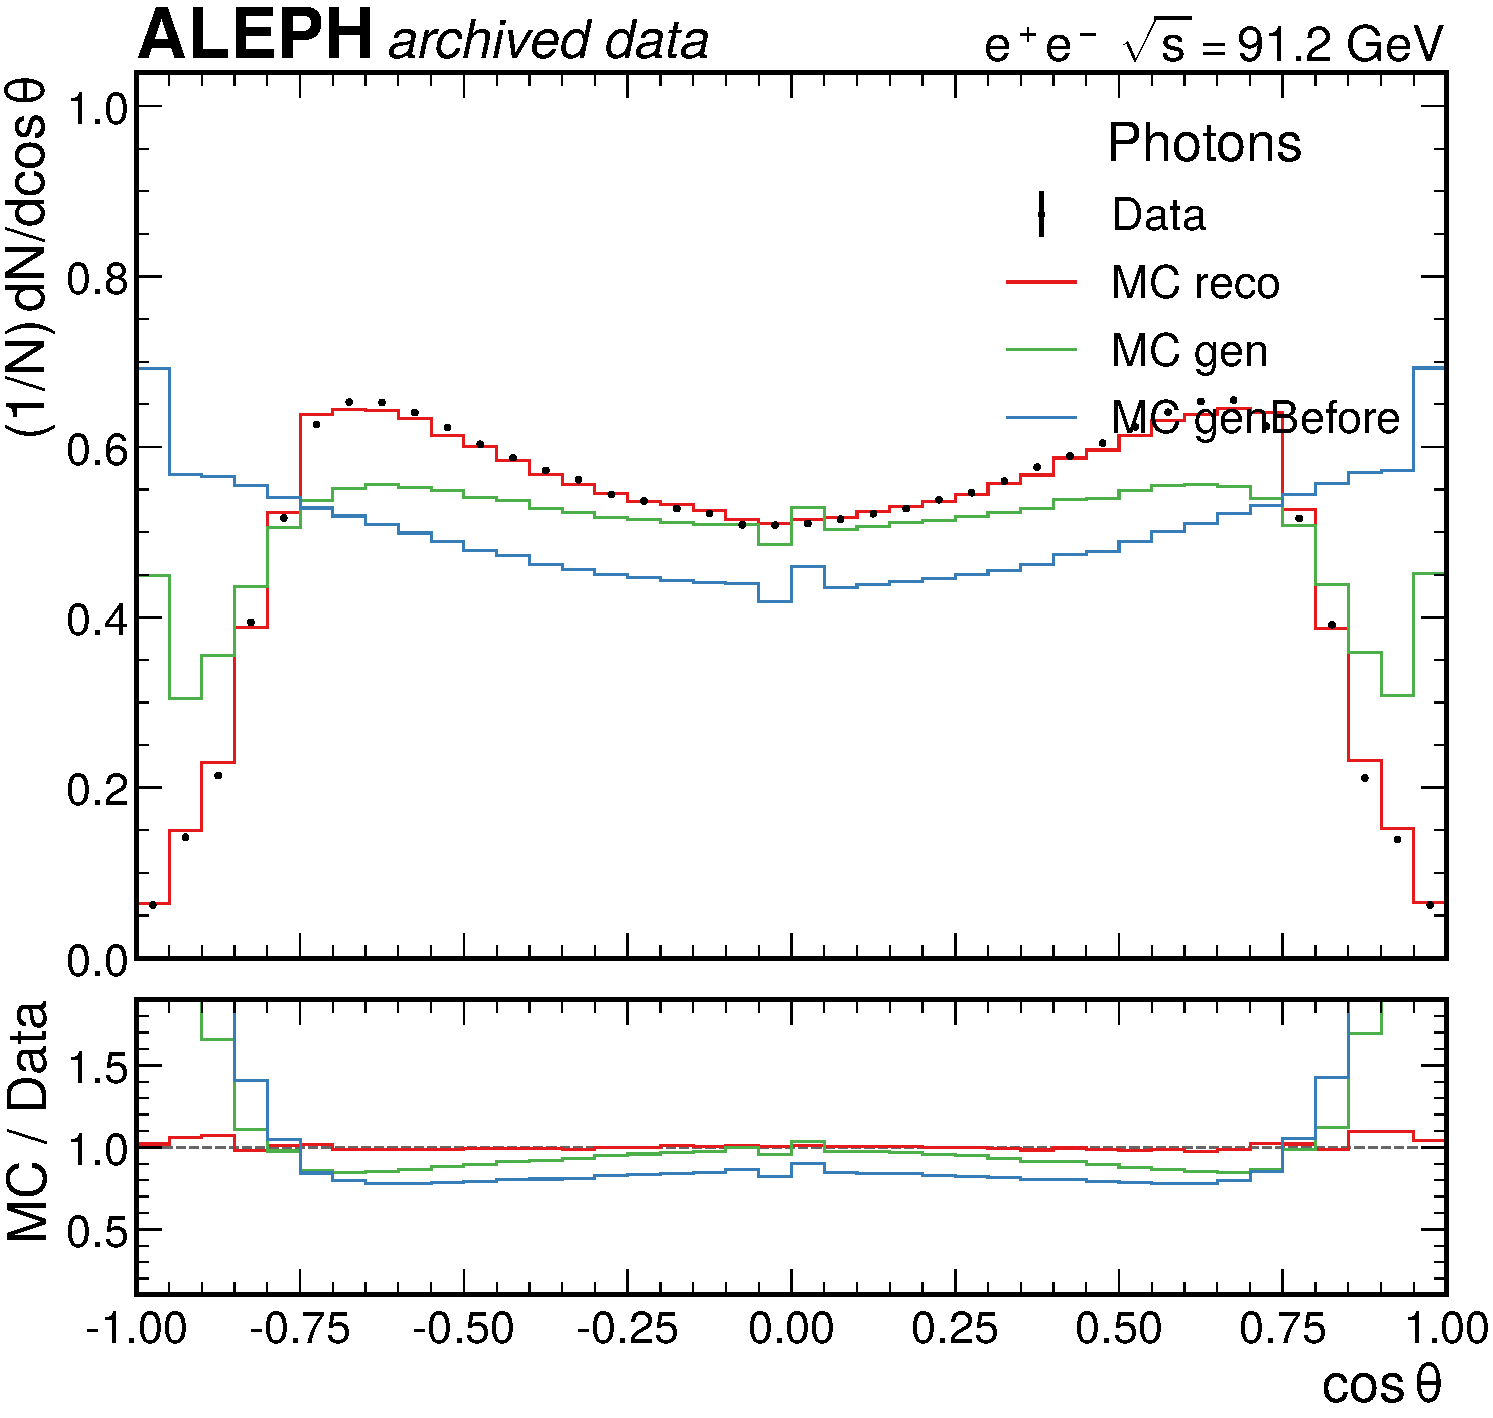
\includegraphics[width=0.495\textwidth]{figures/pwflag4_cosTheta.pdf}
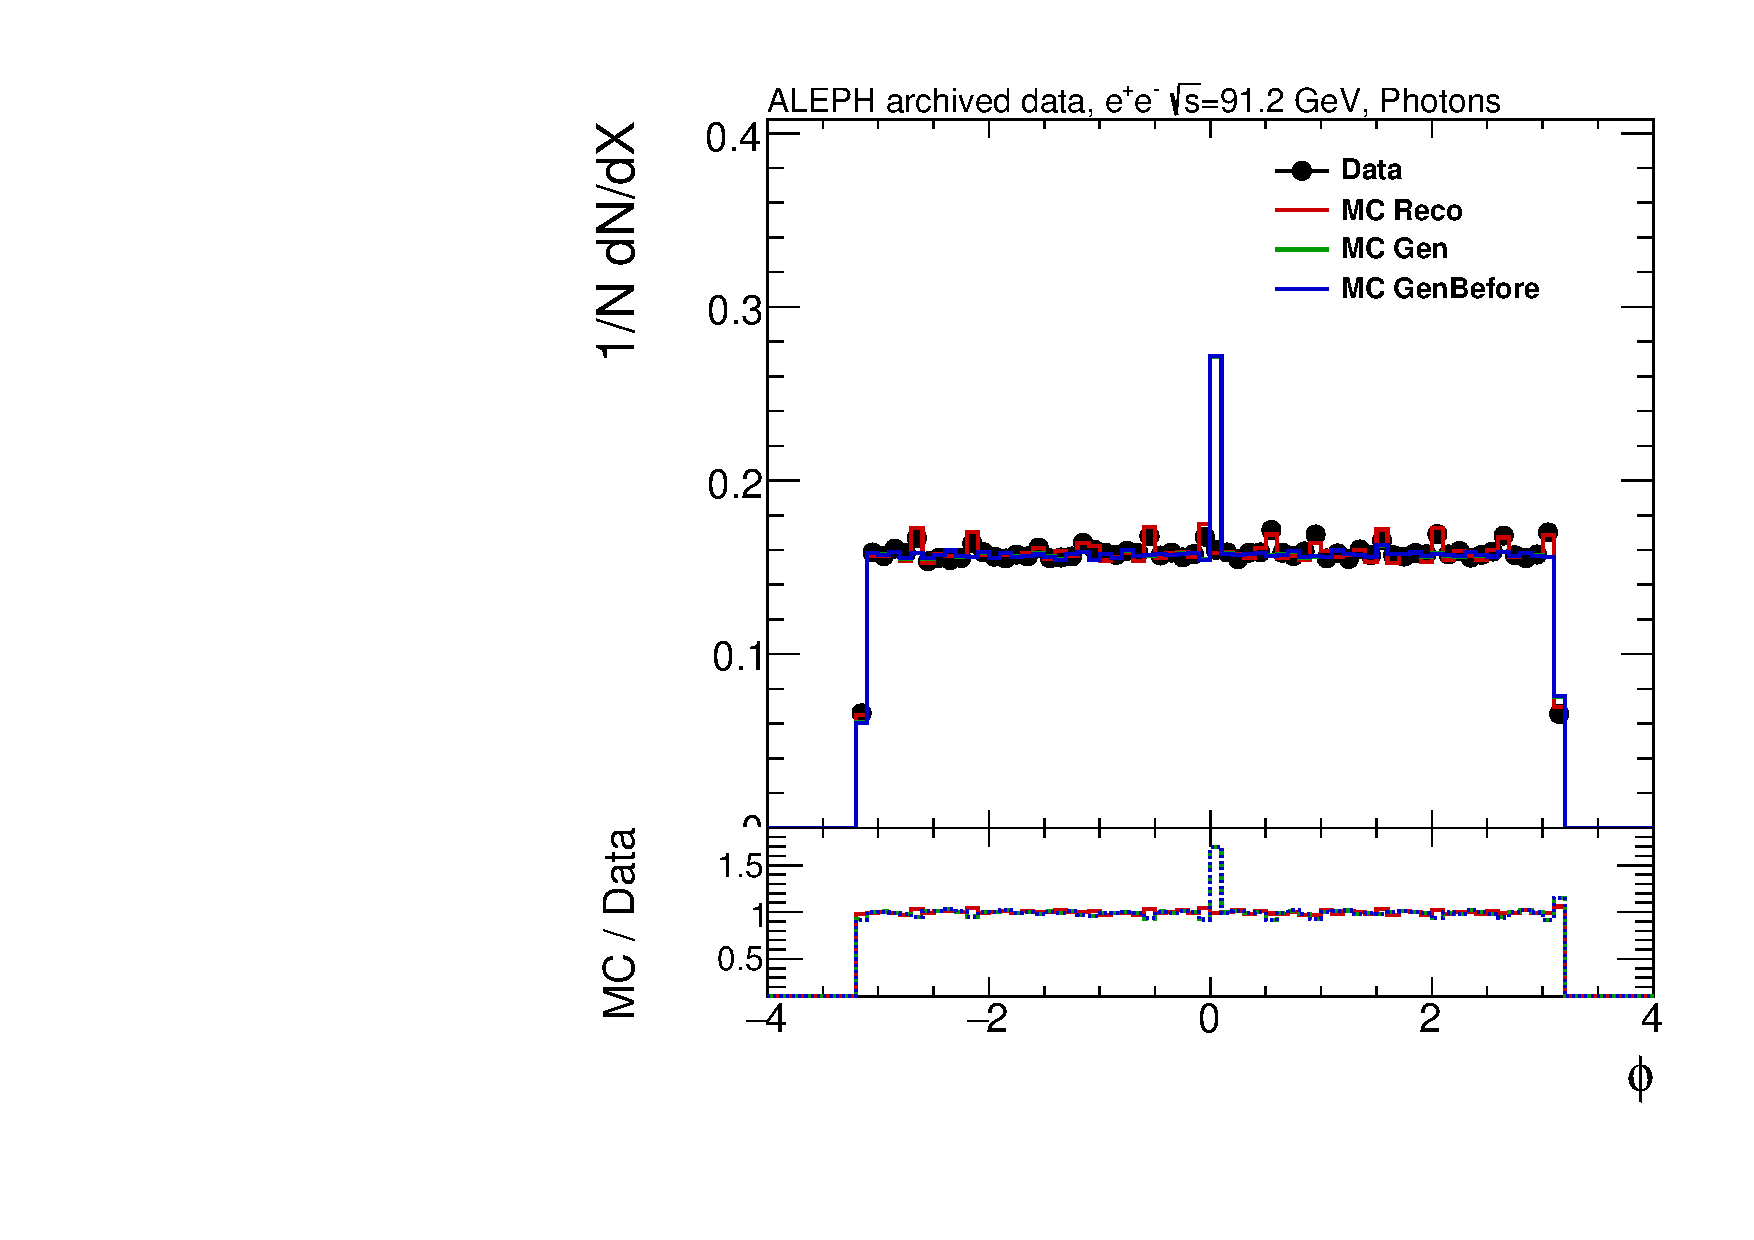
\includegraphics[width=0.495\textwidth]{figures/pwflag4_phi.pdf}
% 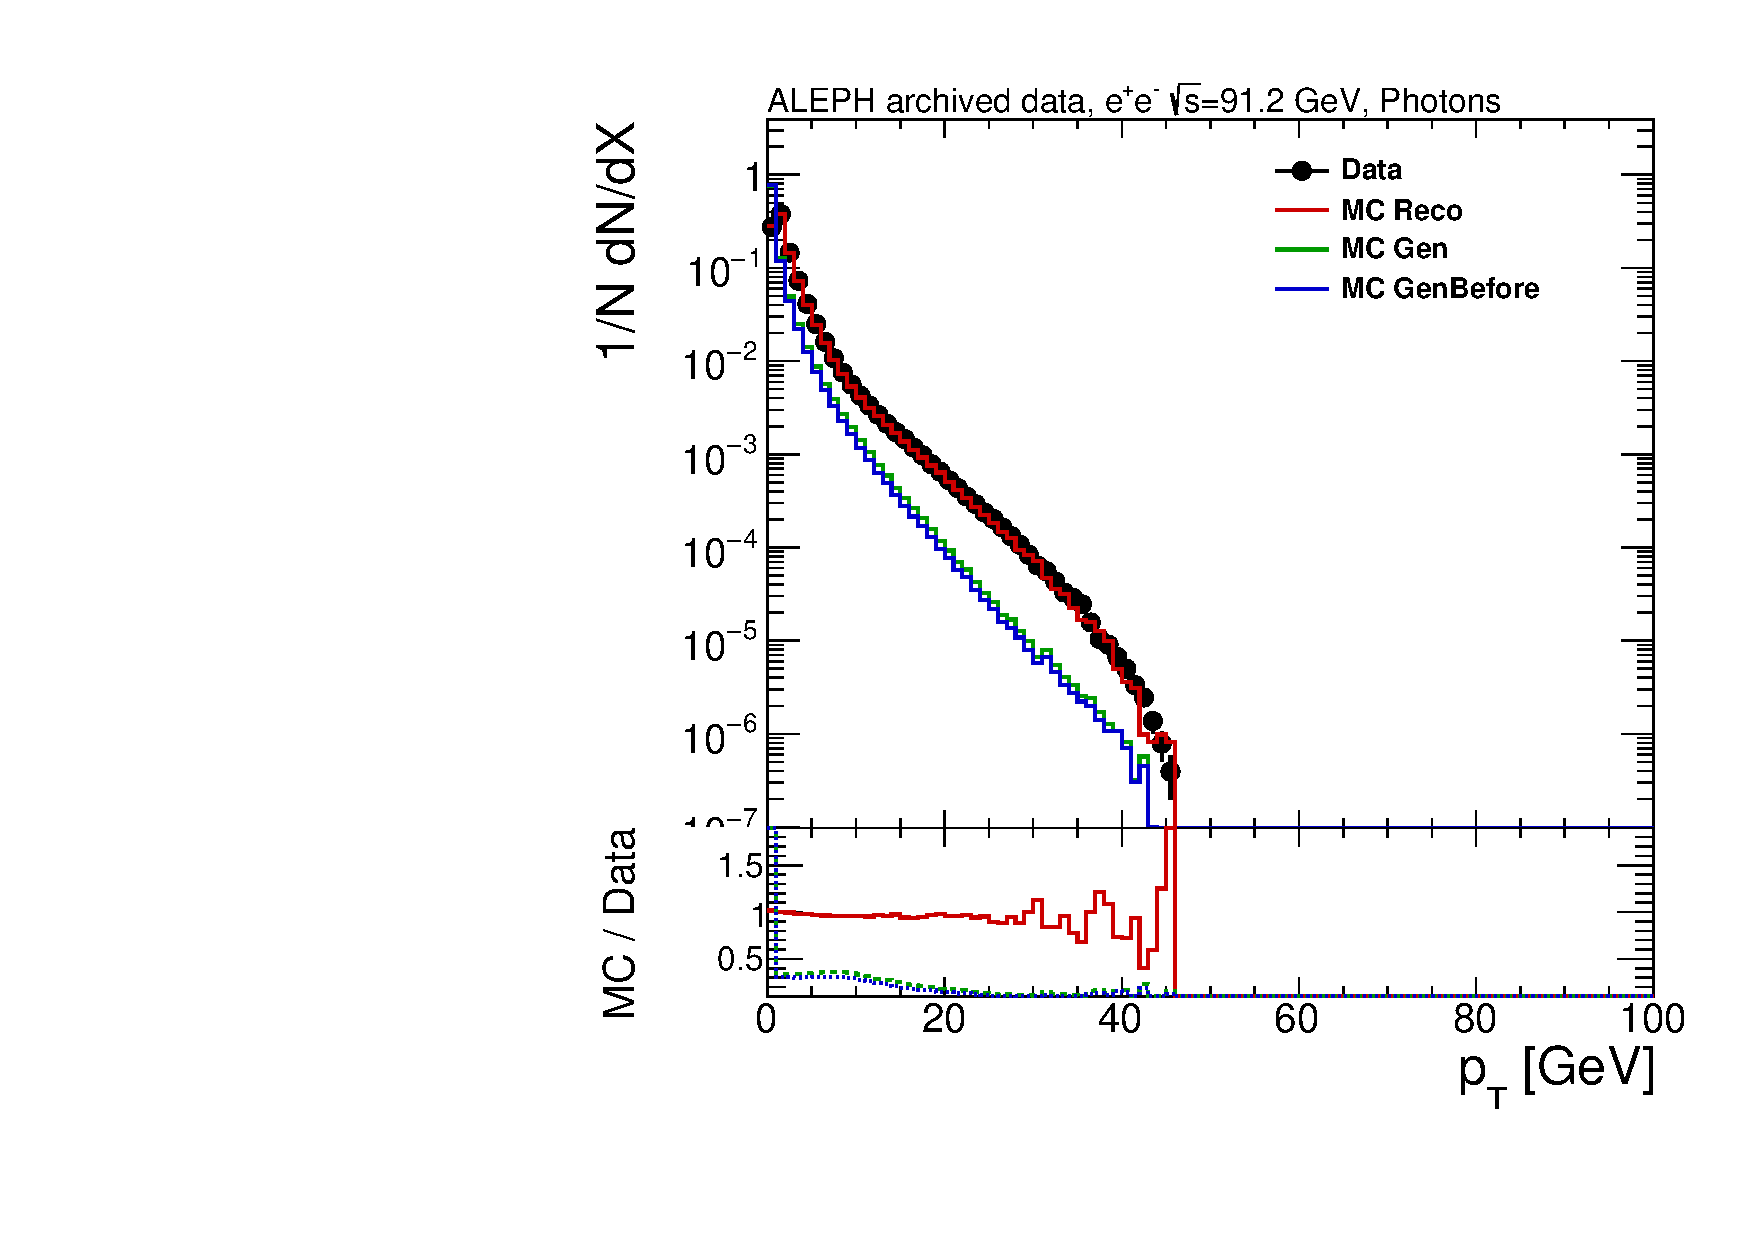
\includegraphics[width=0.242\textwidth]{figures/pwflag4_pt.pdf}
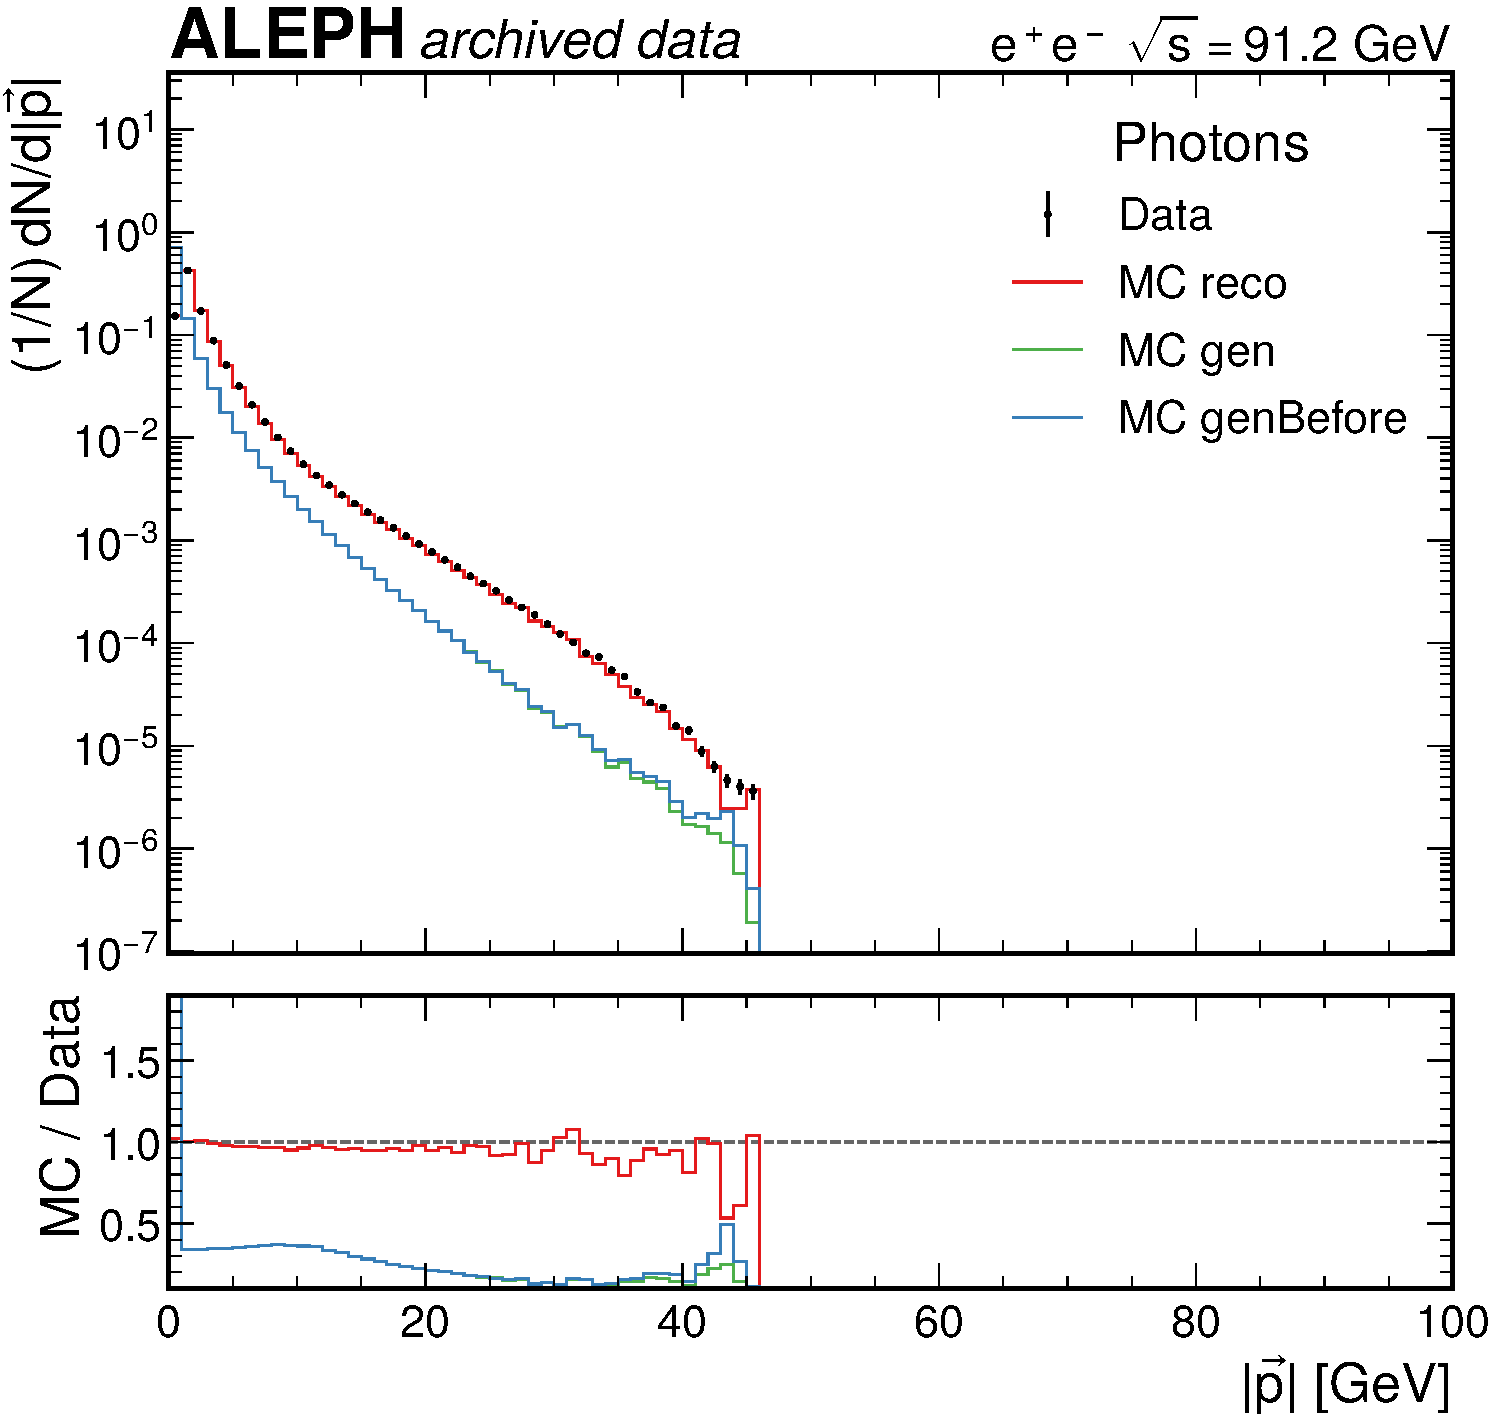
\includegraphics[width=0.495\textwidth]{figures/pwflag4_pmag.pdf}
% 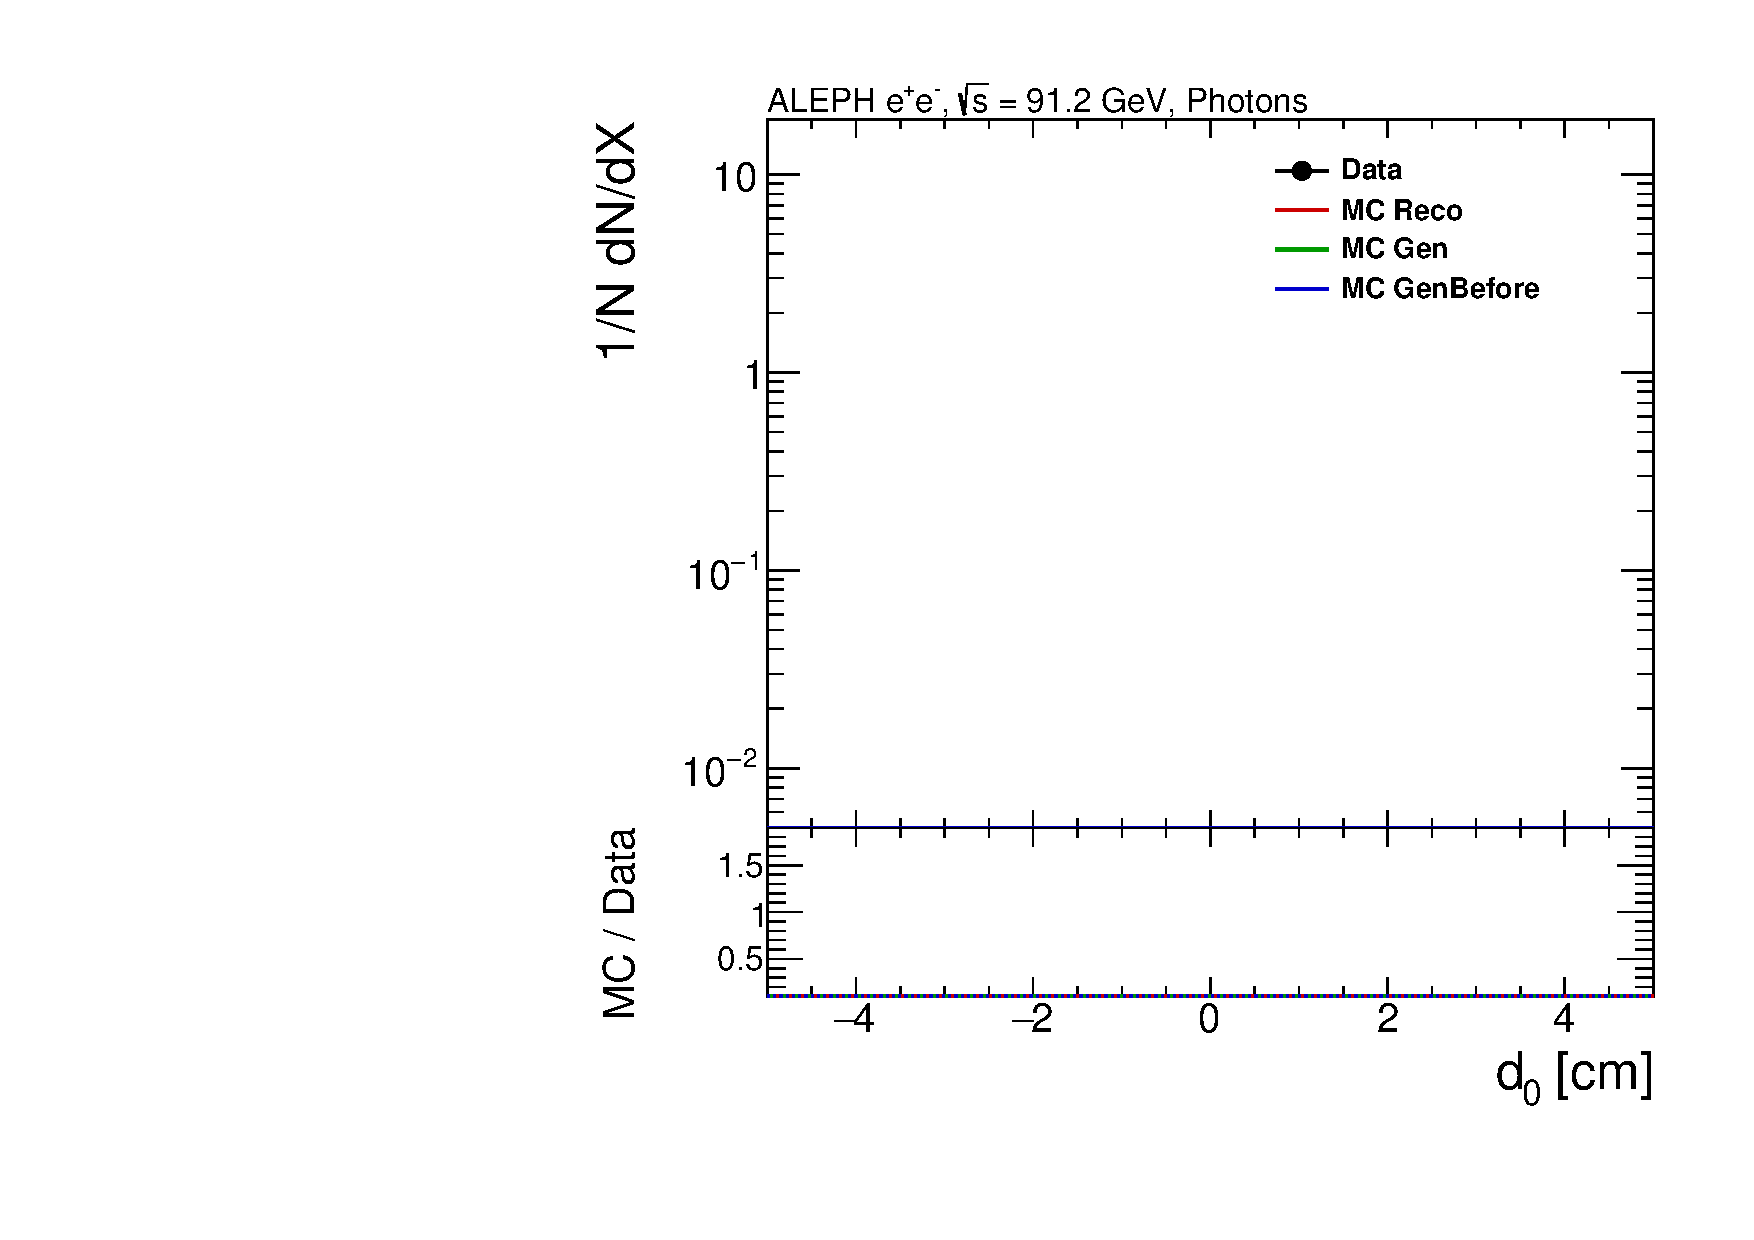
\includegraphics[width=0.242\textwidth]{figures/pwflag4_d0.pdf}
% 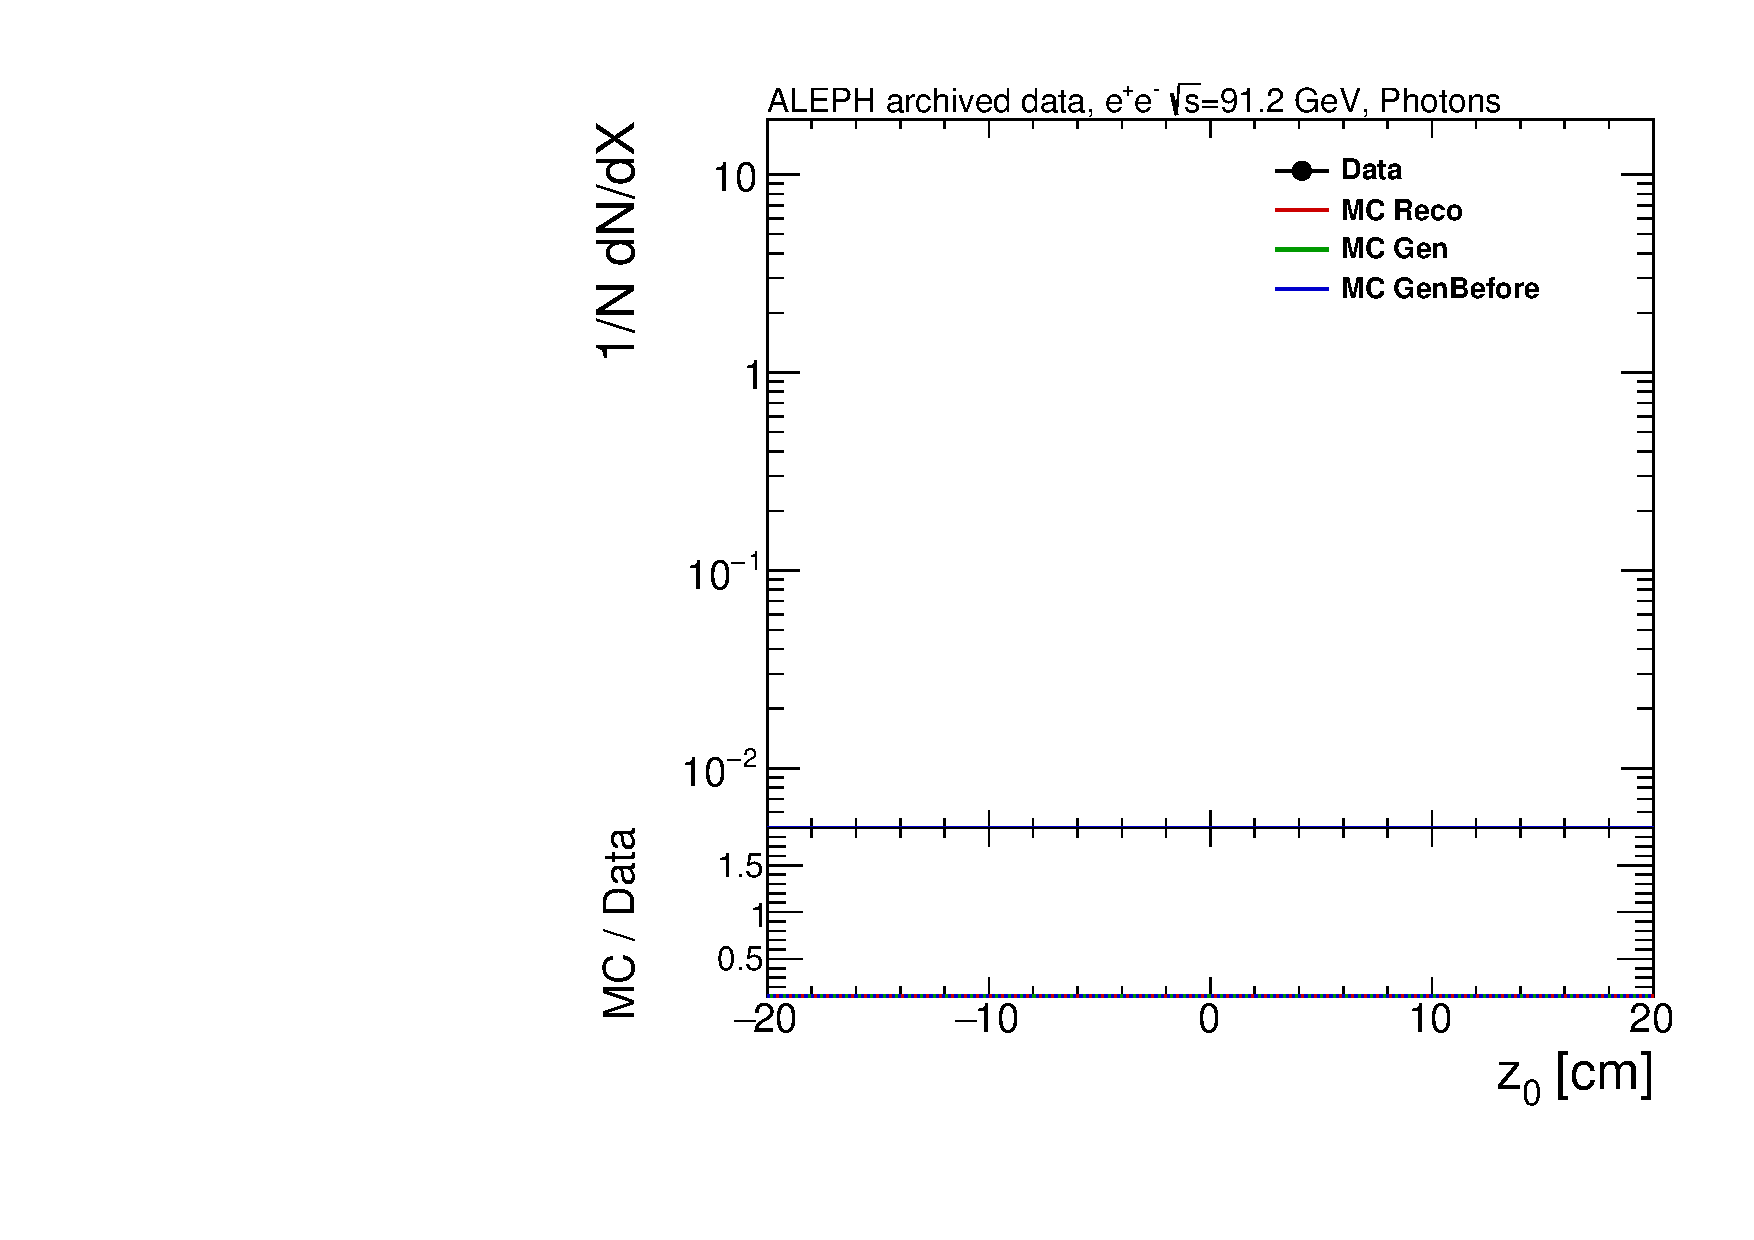
\includegraphics[width=0.242\textwidth]{figures/pwflag4_z0.pdf}
% 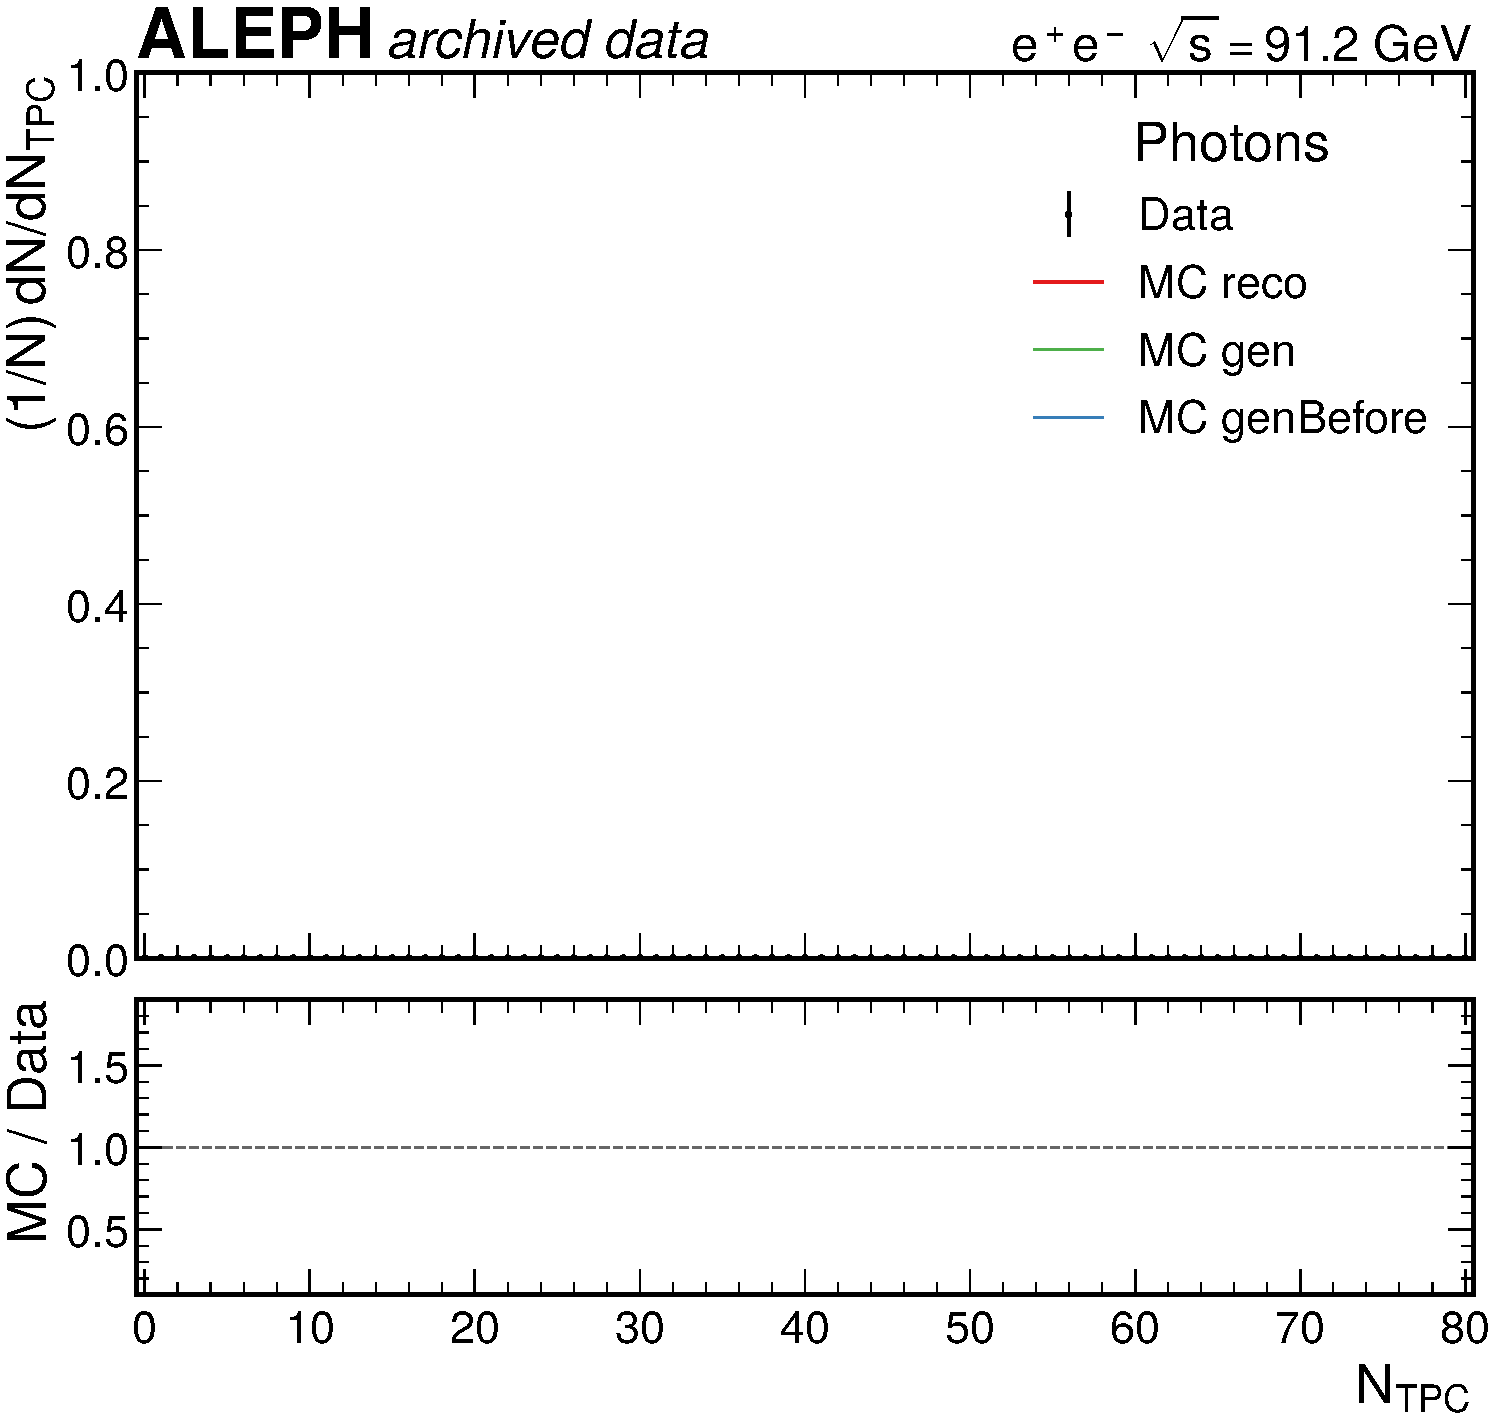
\includegraphics[width=0.242\textwidth]{figures/pwflag4_ntpc.pdf}
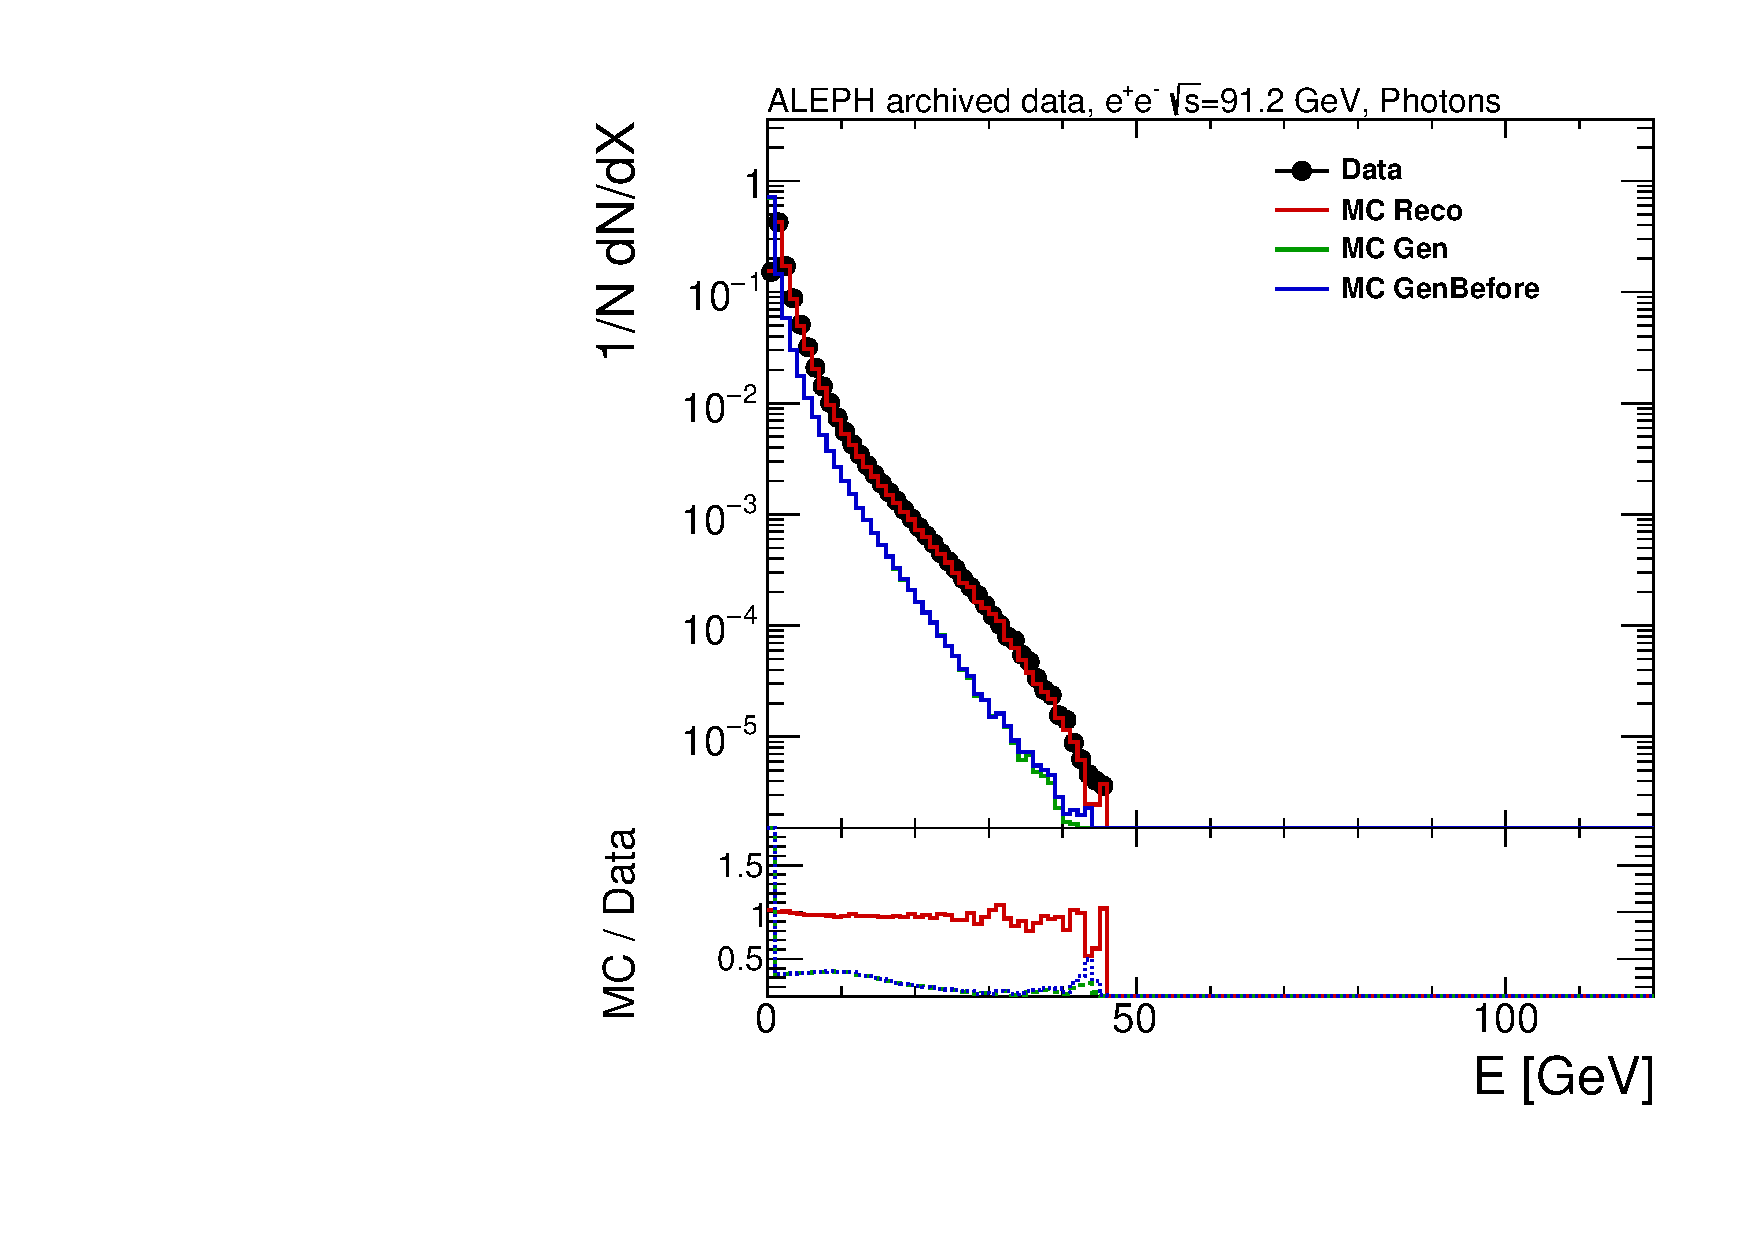
\includegraphics[width=0.495\textwidth]{figures/pwflag4_energy.pdf}
% 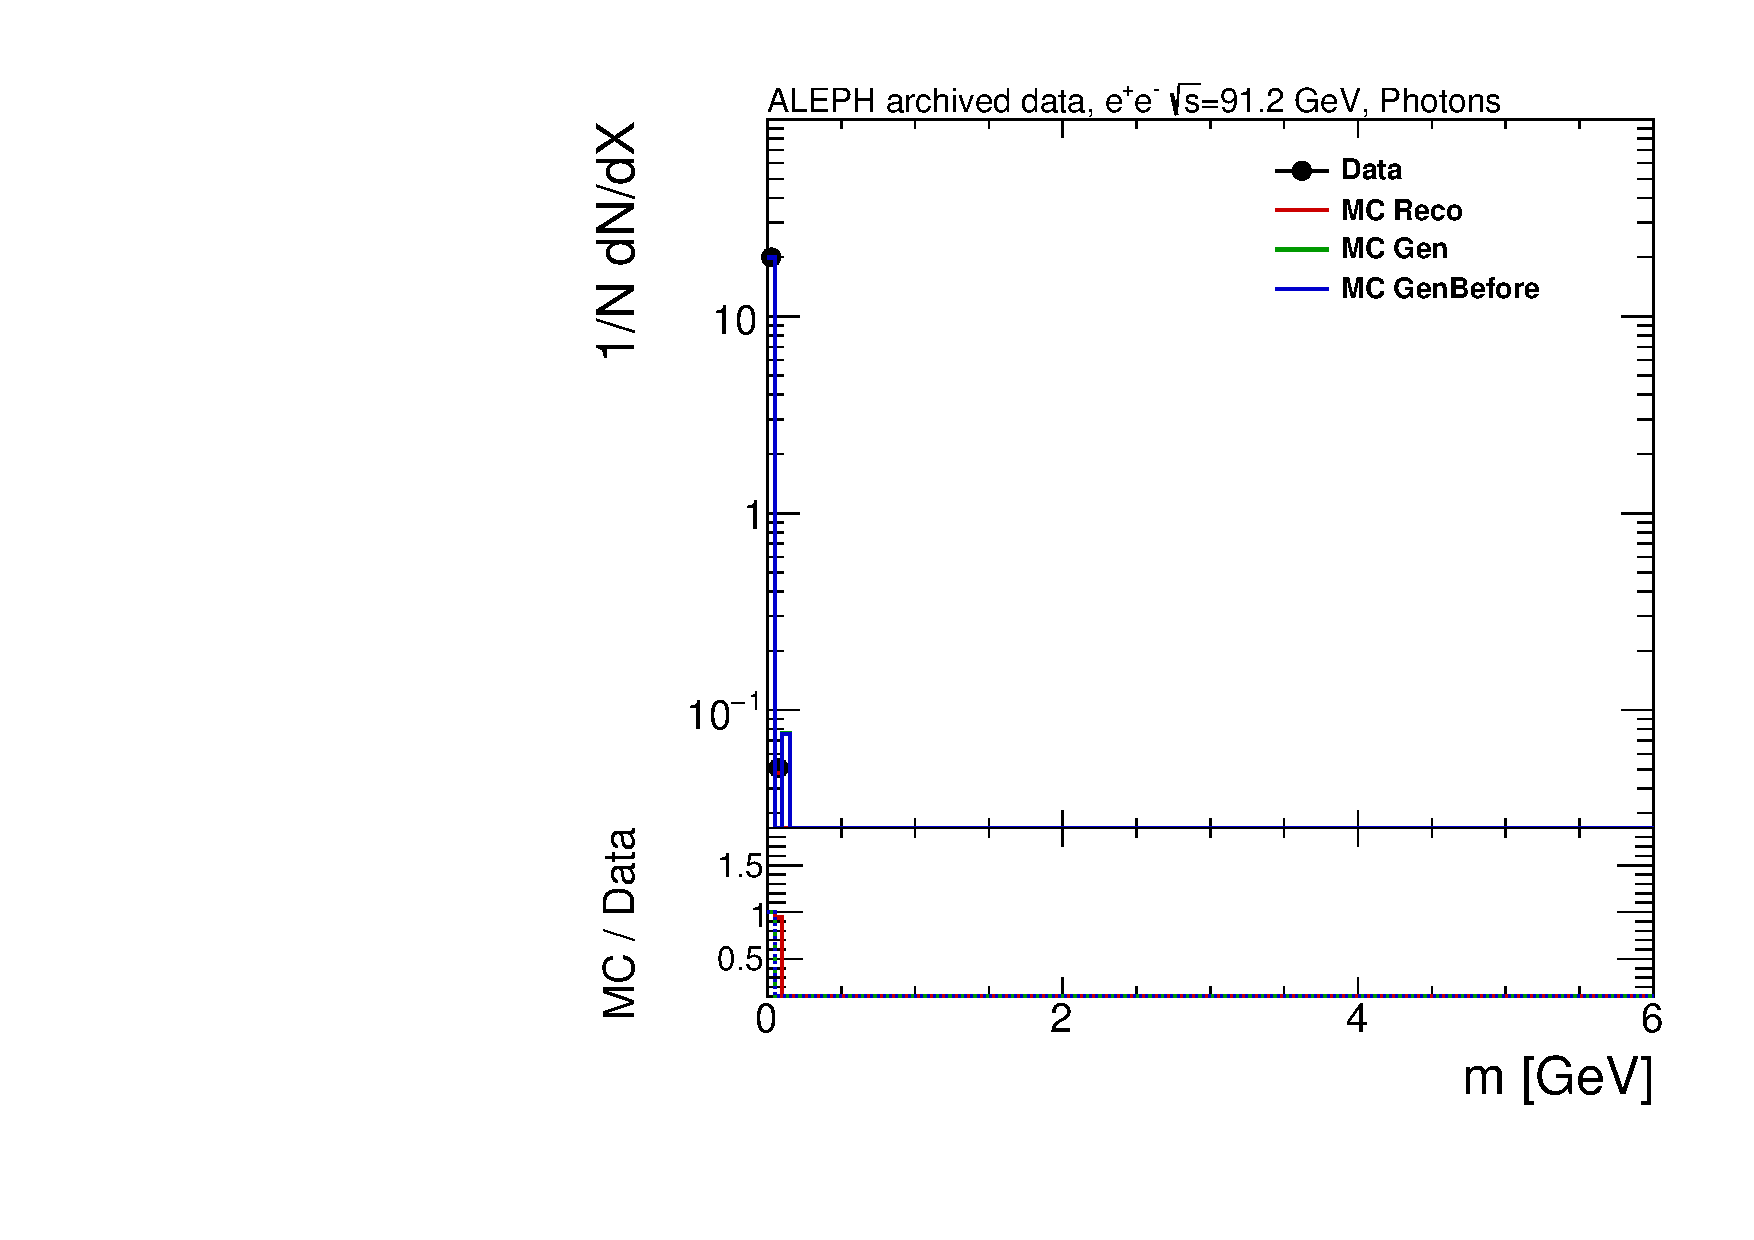
\includegraphics[width=0.495\textwidth]{figures/pwflag4_mass.pdf}
\caption{Complete \texttt{pwflag}=4 kinematic set.}
\label{fig:pwflag4_full}
\end{figure}

\FloatBarrier

\begin{figure}[t!]
\centering
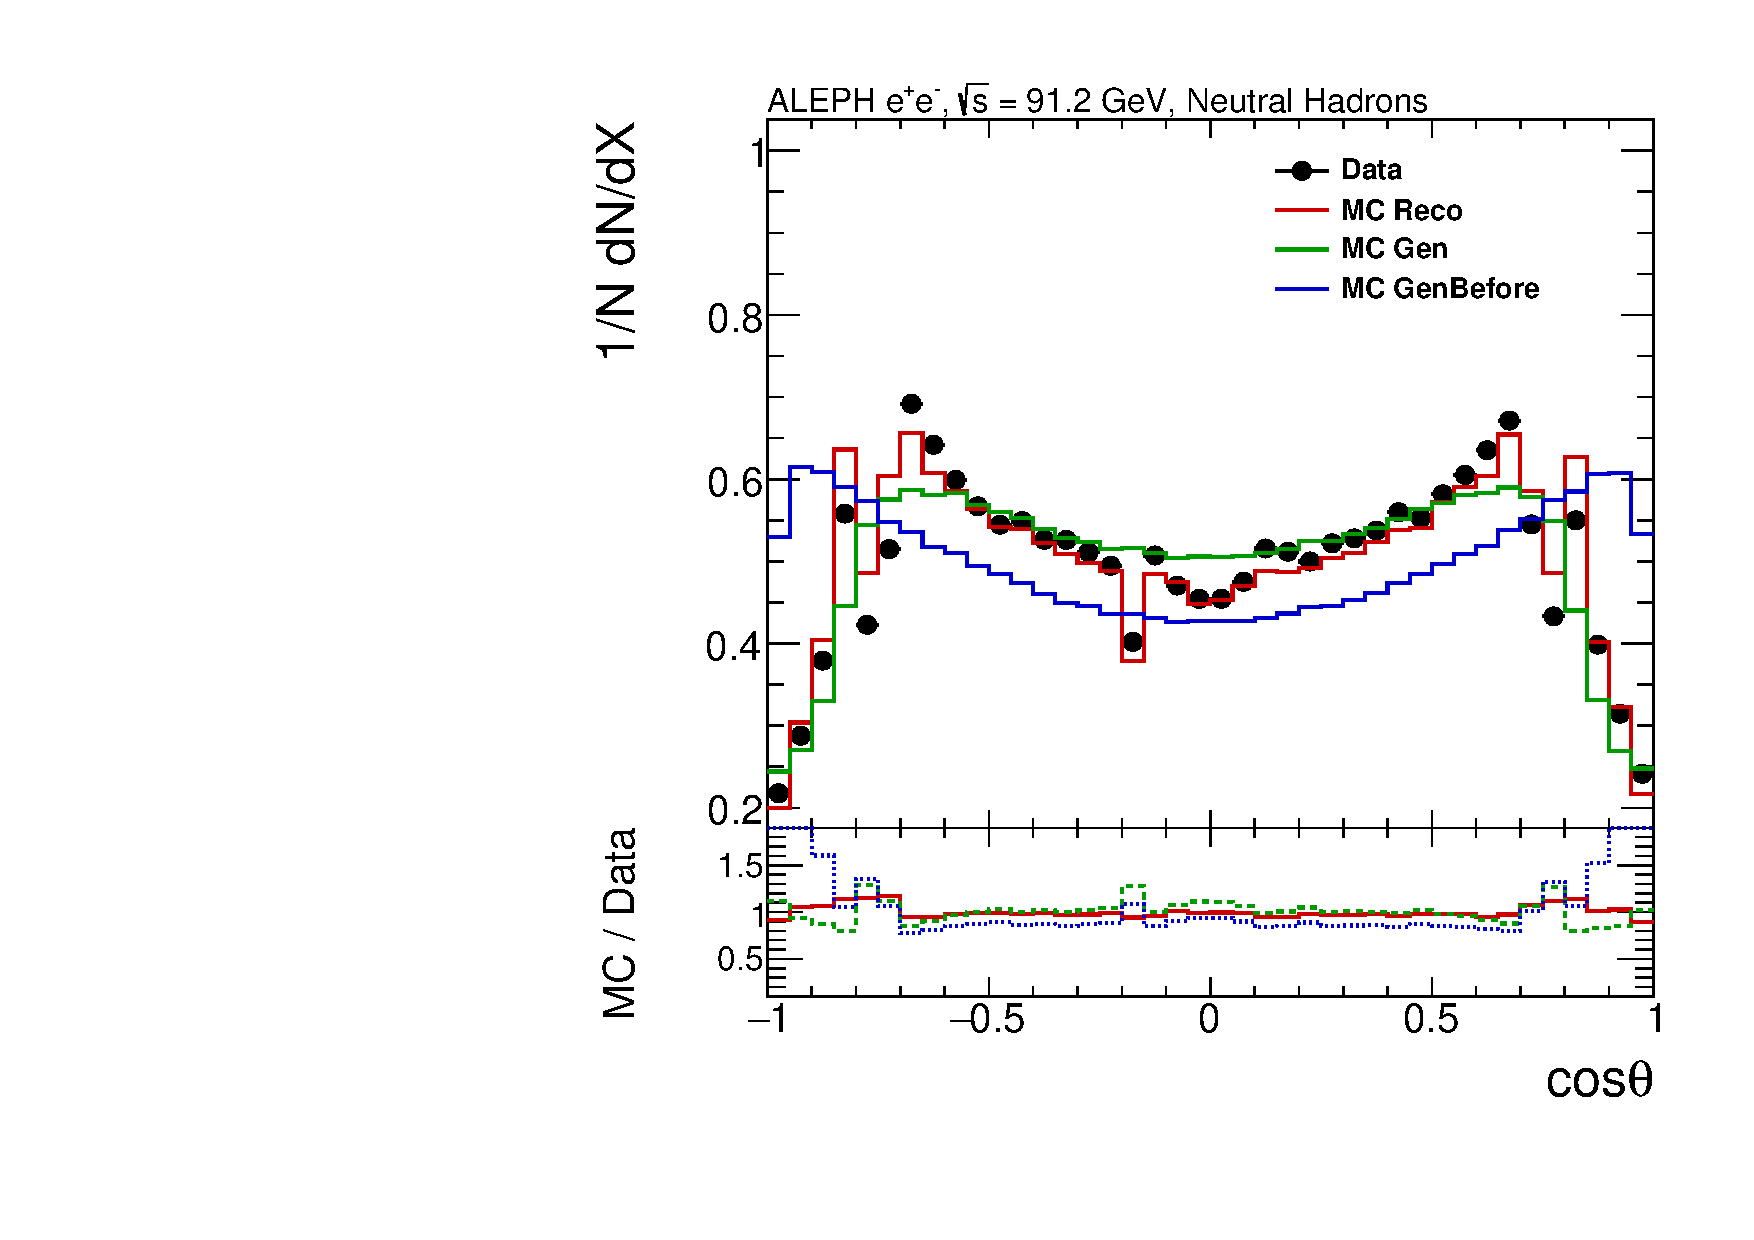
\includegraphics[width=0.495\textwidth]{figures/pwflag5_cosTheta.pdf}
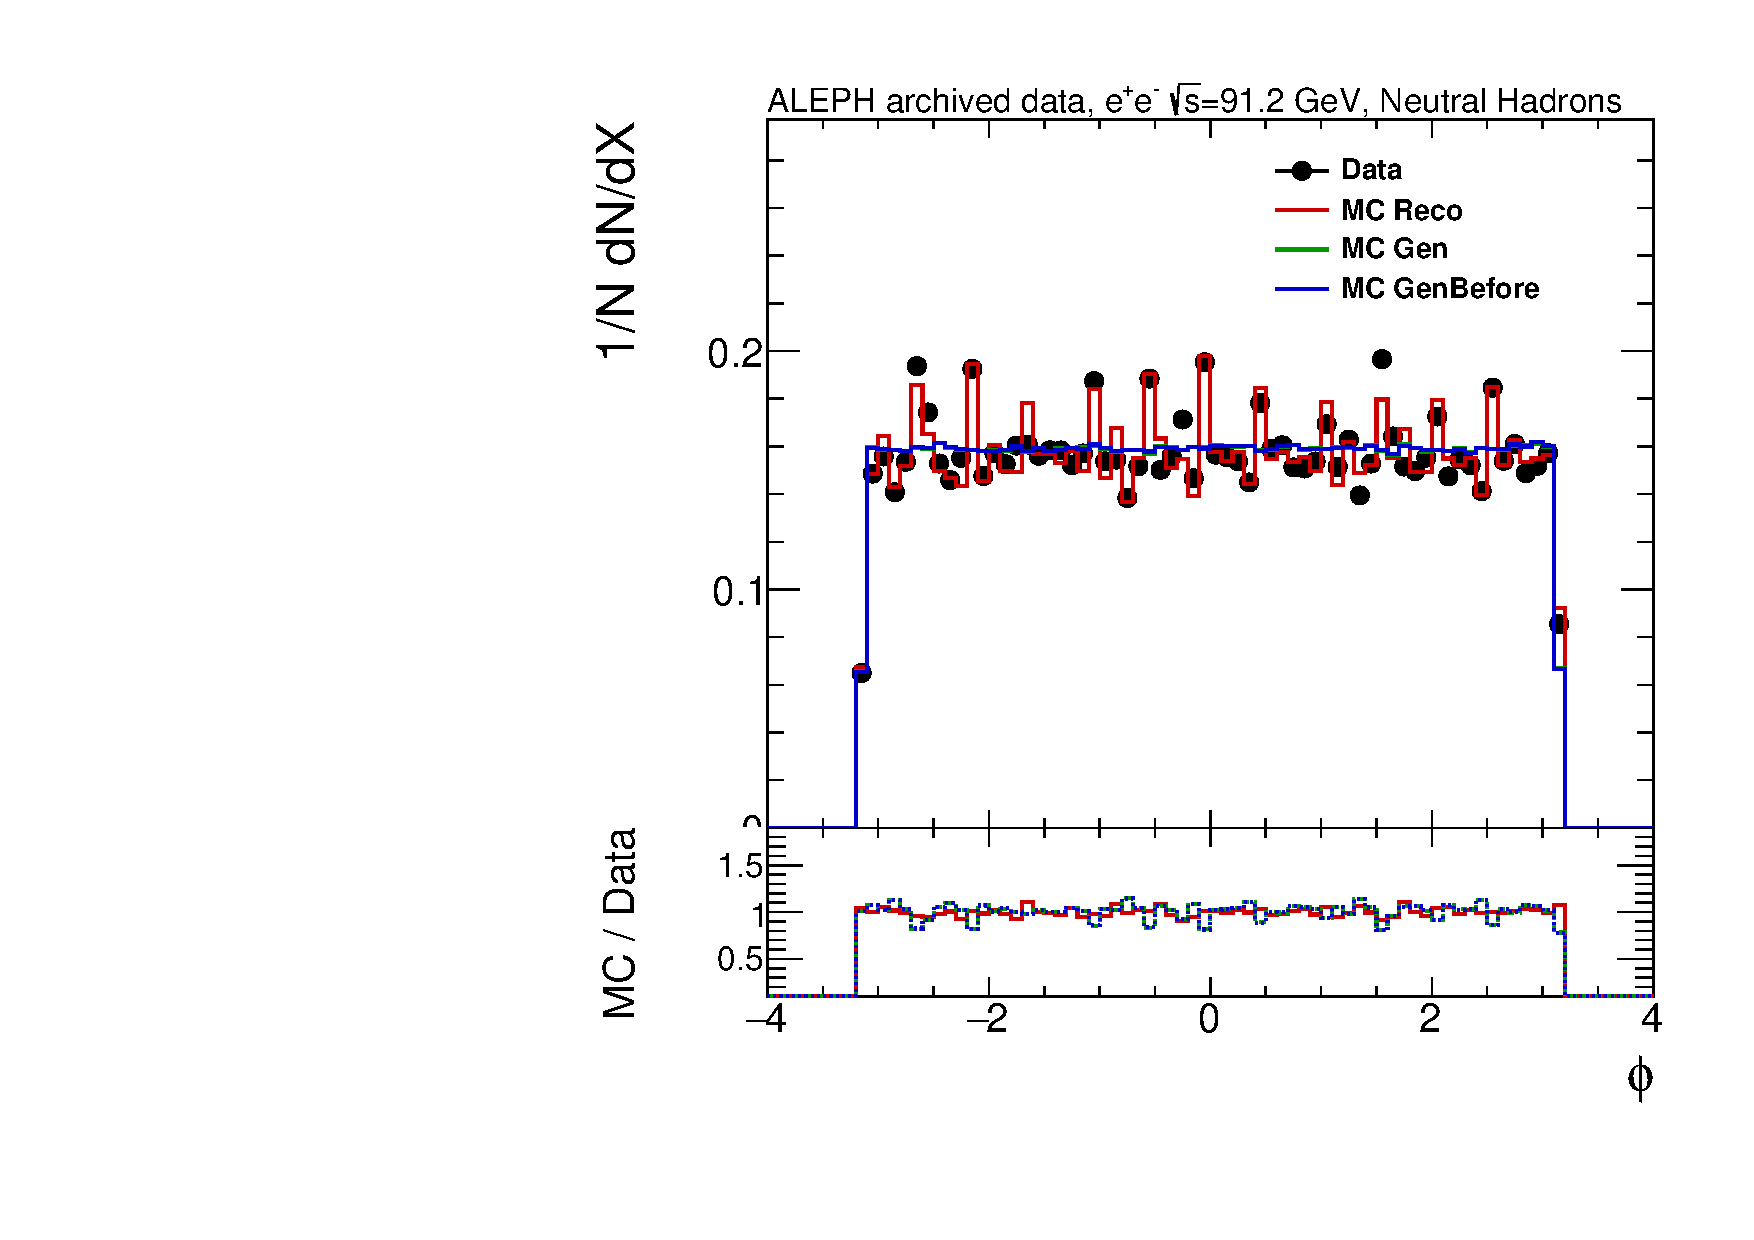
\includegraphics[width=0.495\textwidth]{figures/pwflag5_phi.pdf}
% 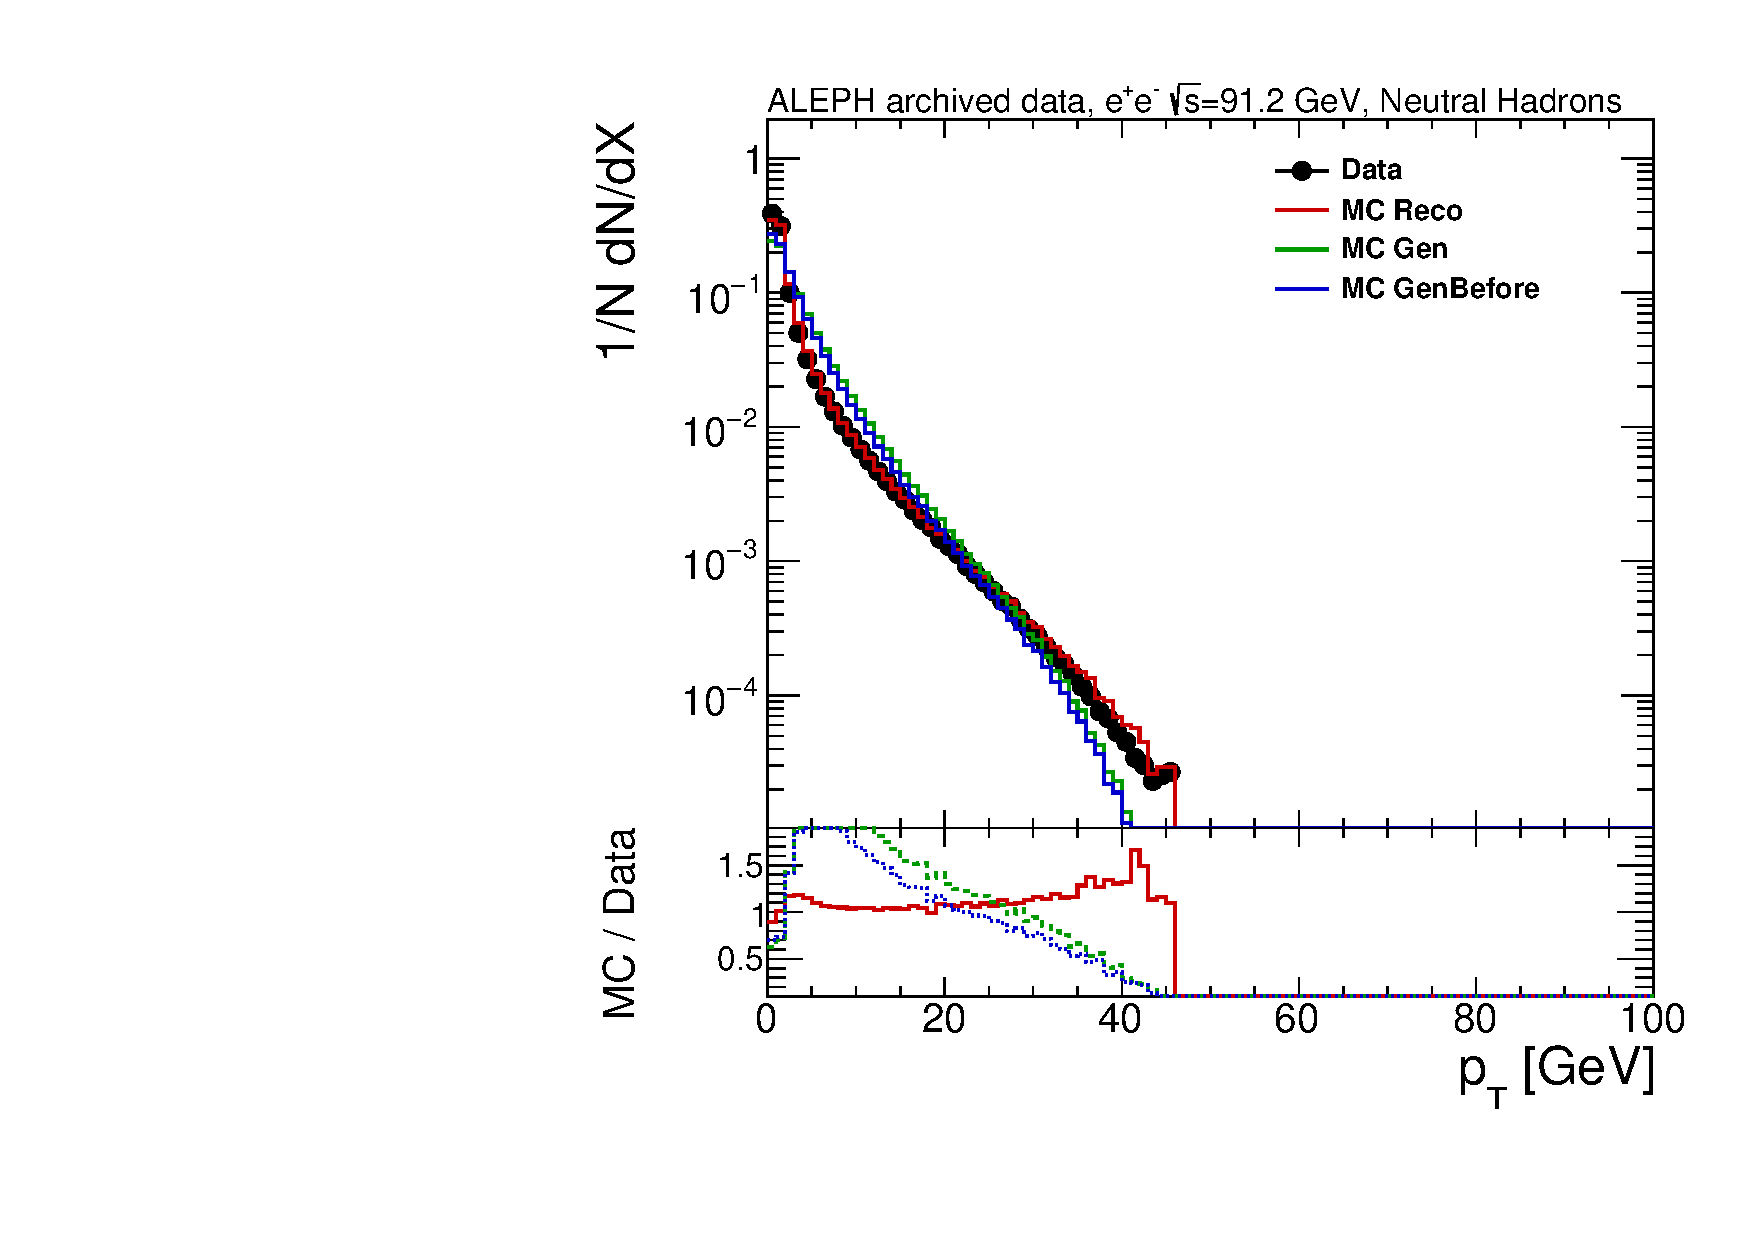
\includegraphics[width=0.242\textwidth]{figures/pwflag5_pt.pdf}
% 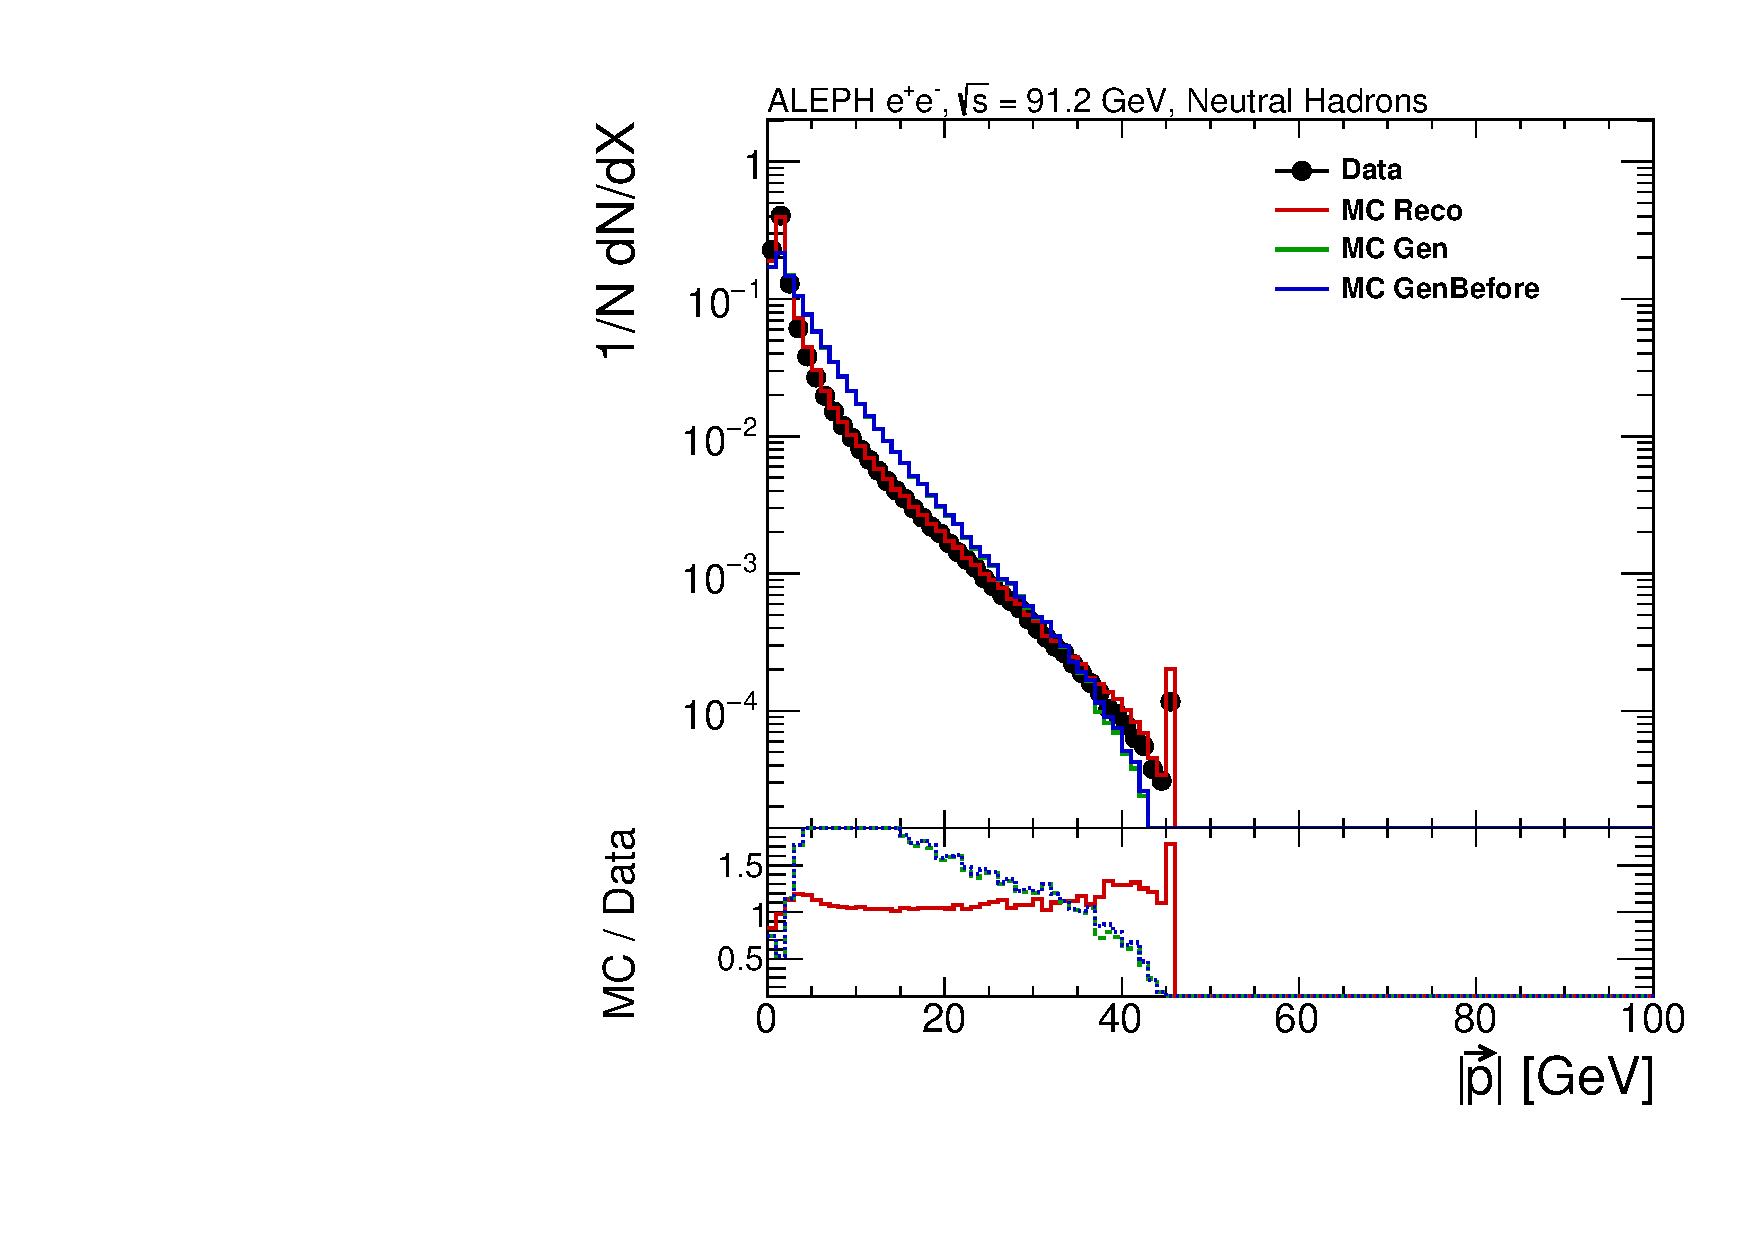
\includegraphics[width=0.242\textwidth]{figures/pwflag5_pmag.pdf}
% 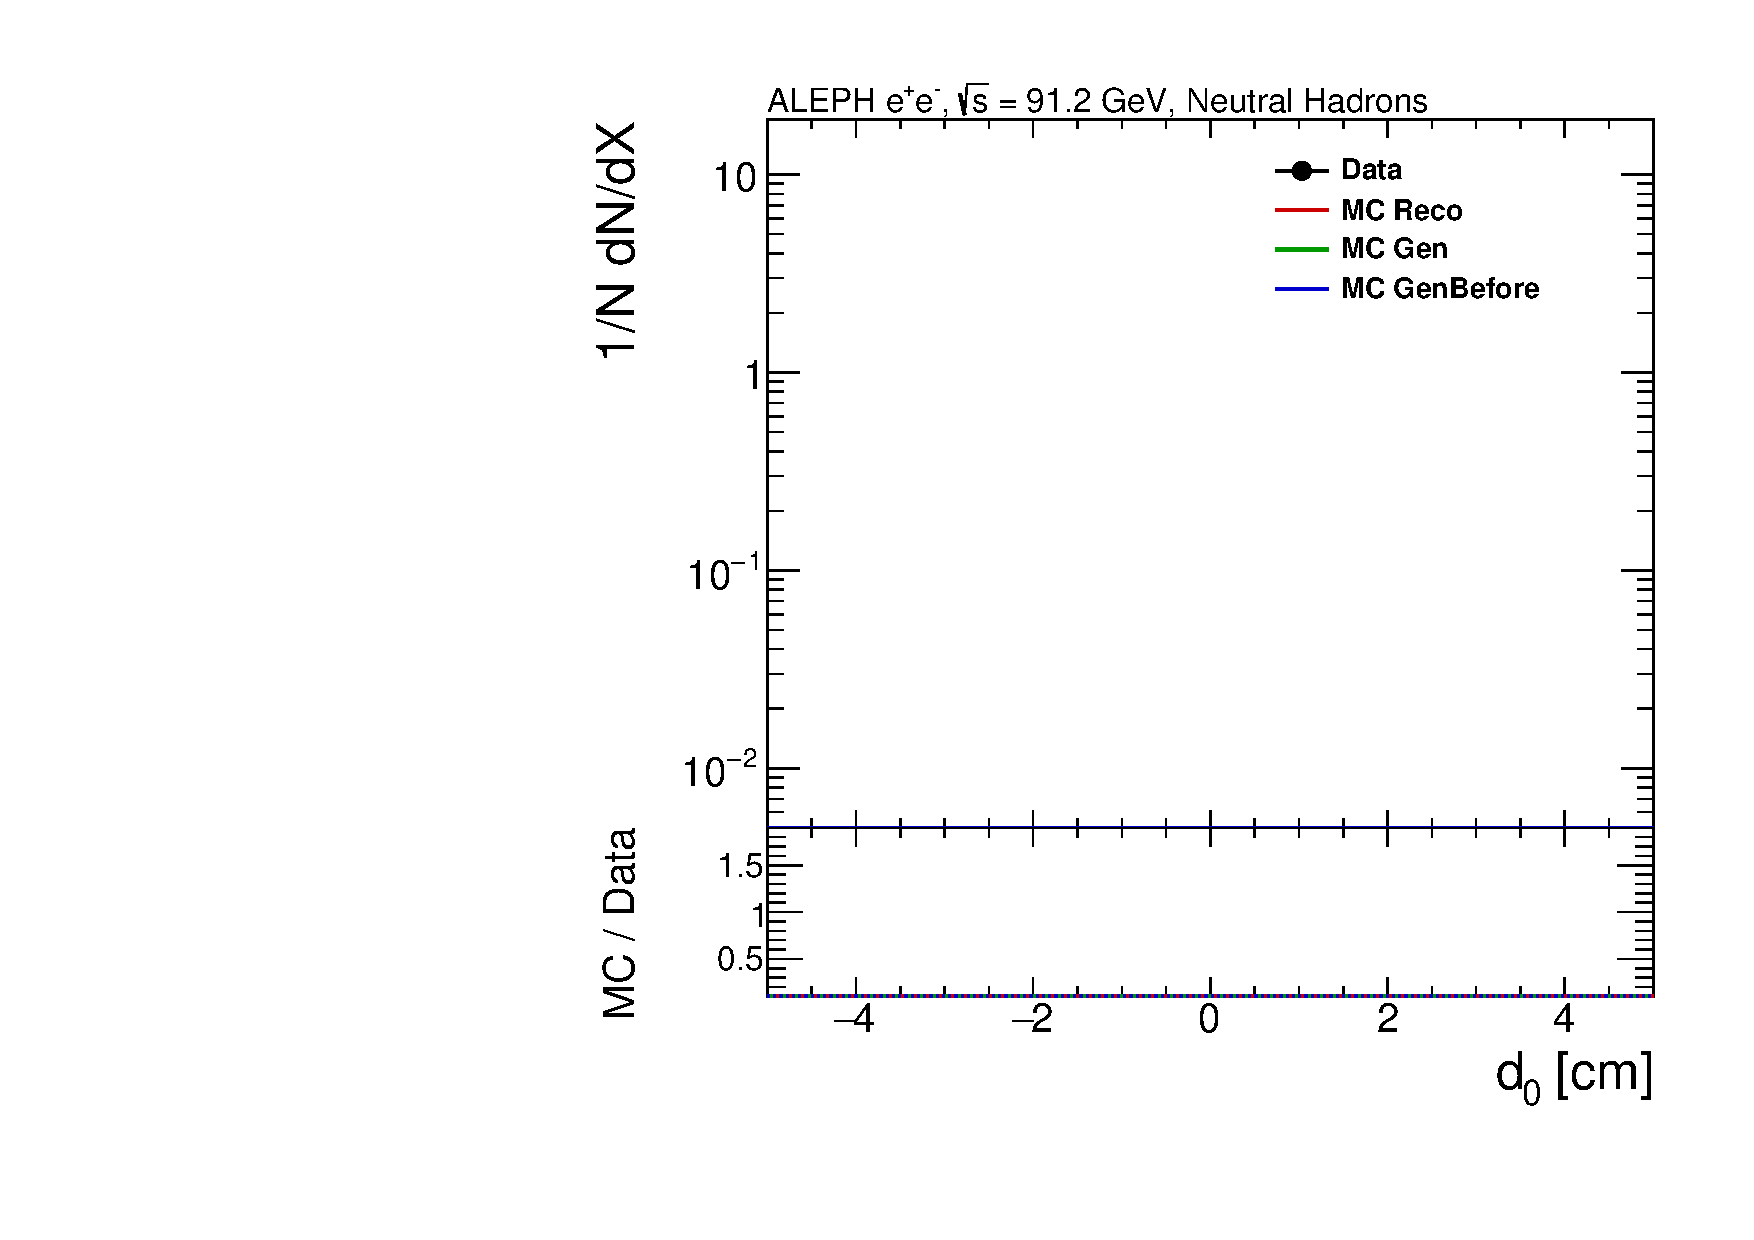
\includegraphics[width=0.242\textwidth]{figures/pwflag5_d0.pdf}
% 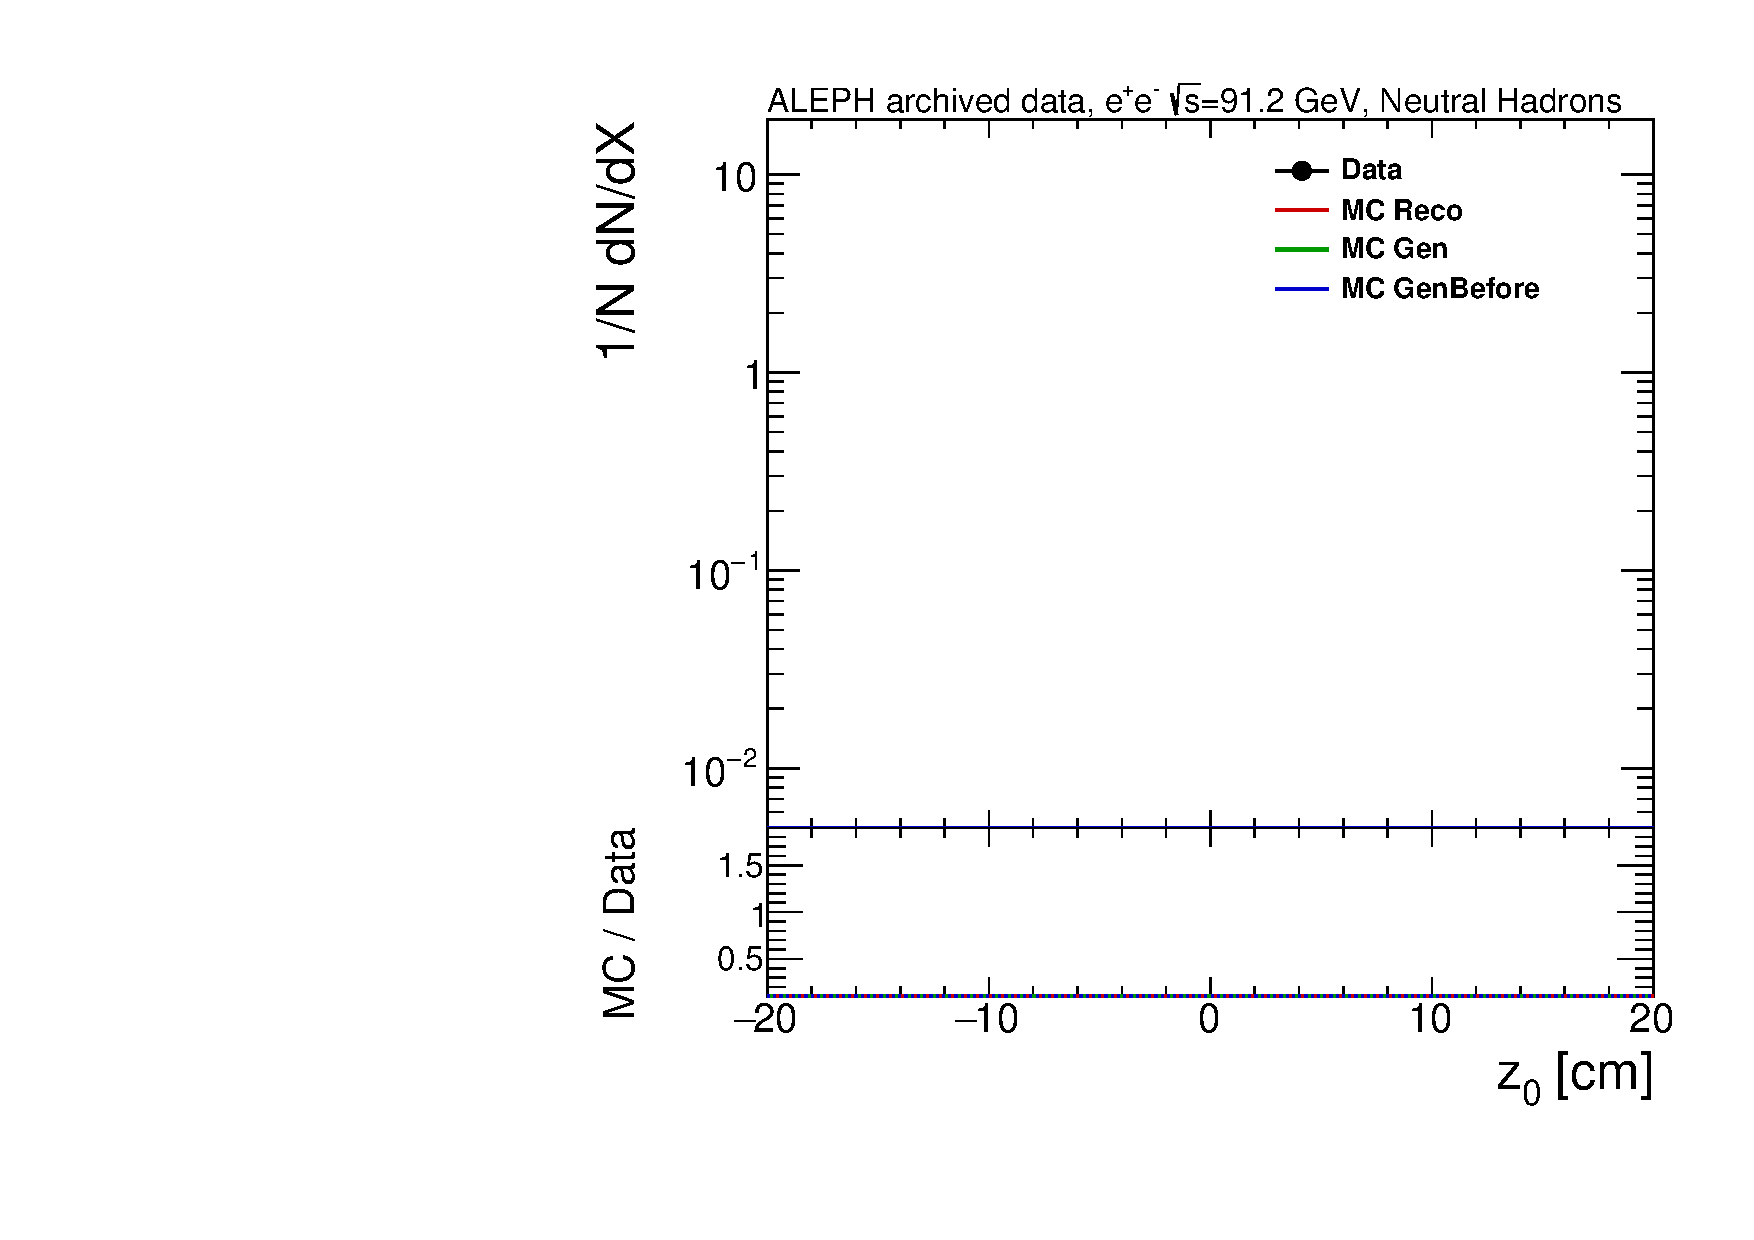
\includegraphics[width=0.242\textwidth]{figures/pwflag5_z0.pdf}
% 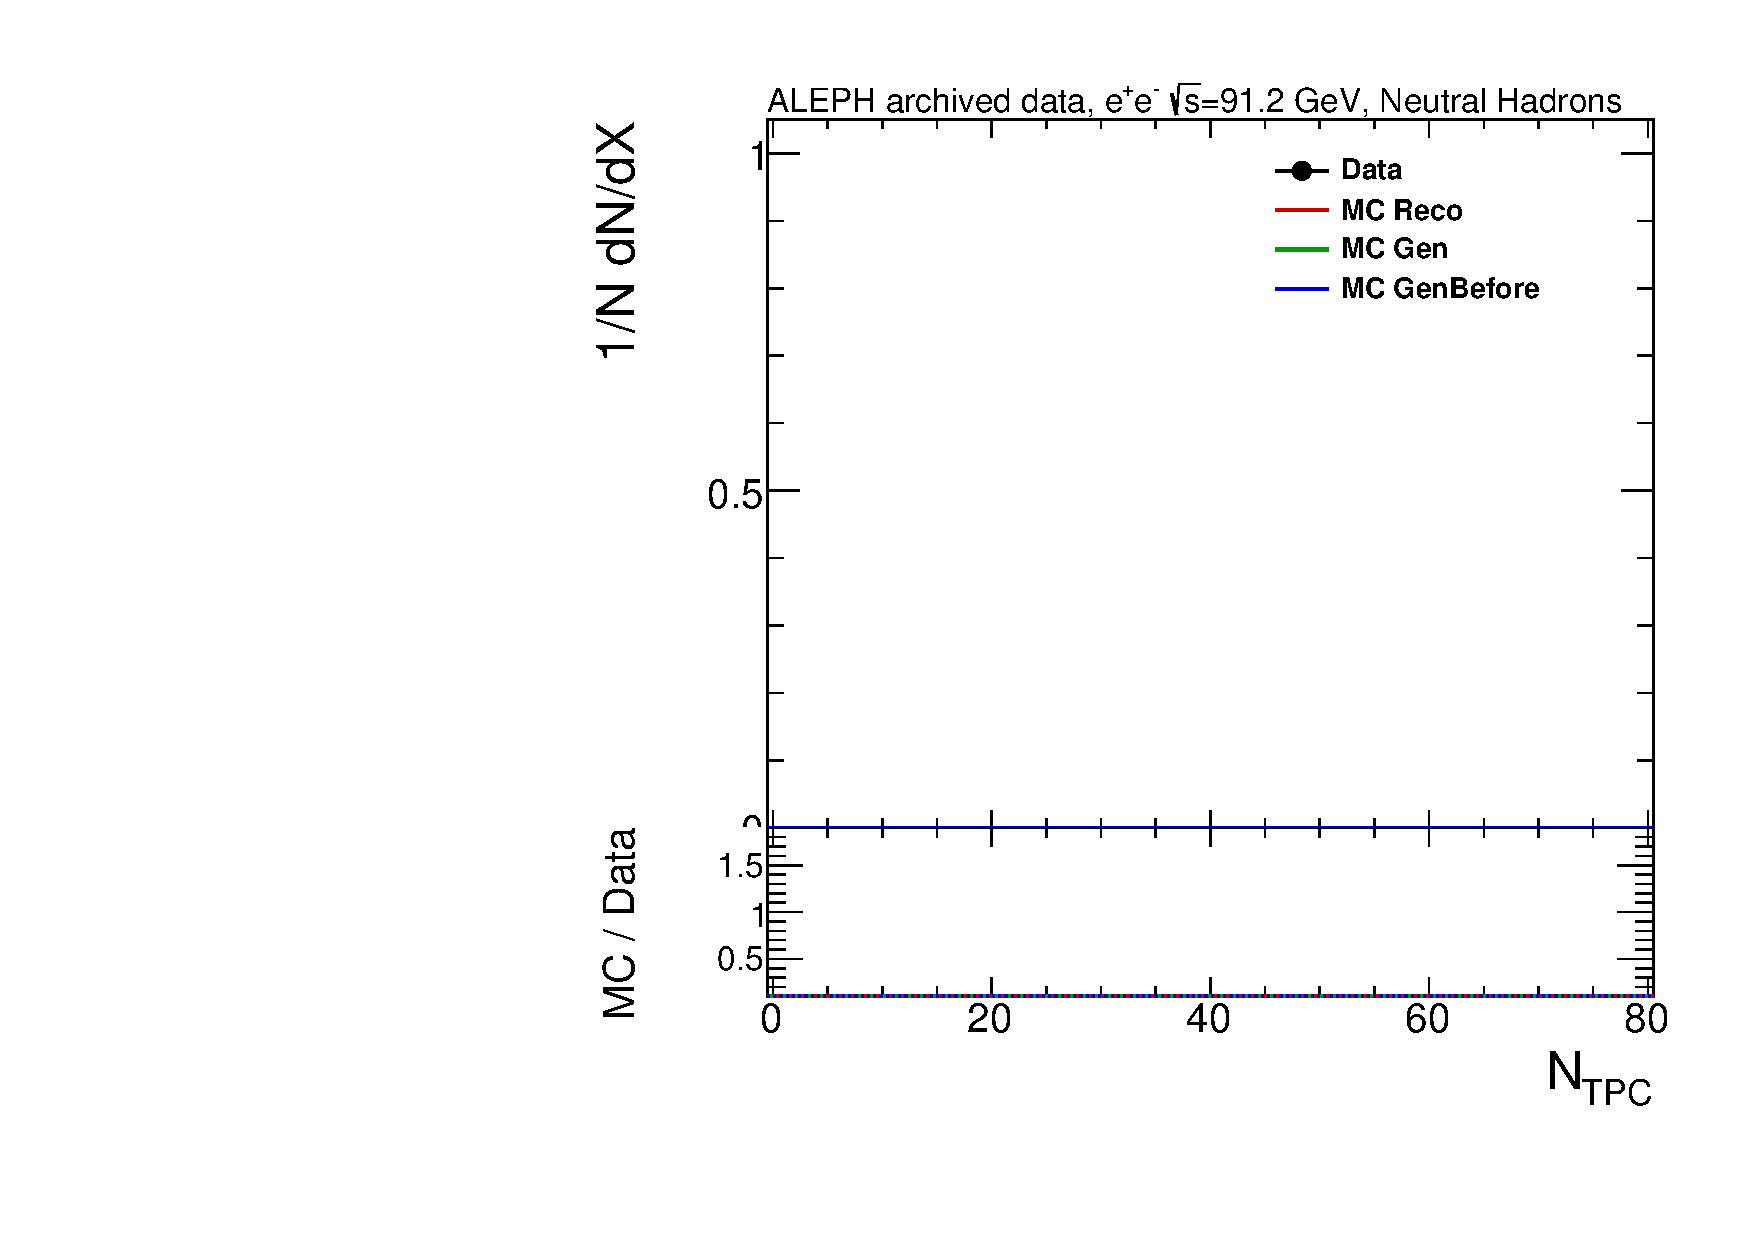
\includegraphics[width=0.242\textwidth]{figures/pwflag5_ntpc.pdf}
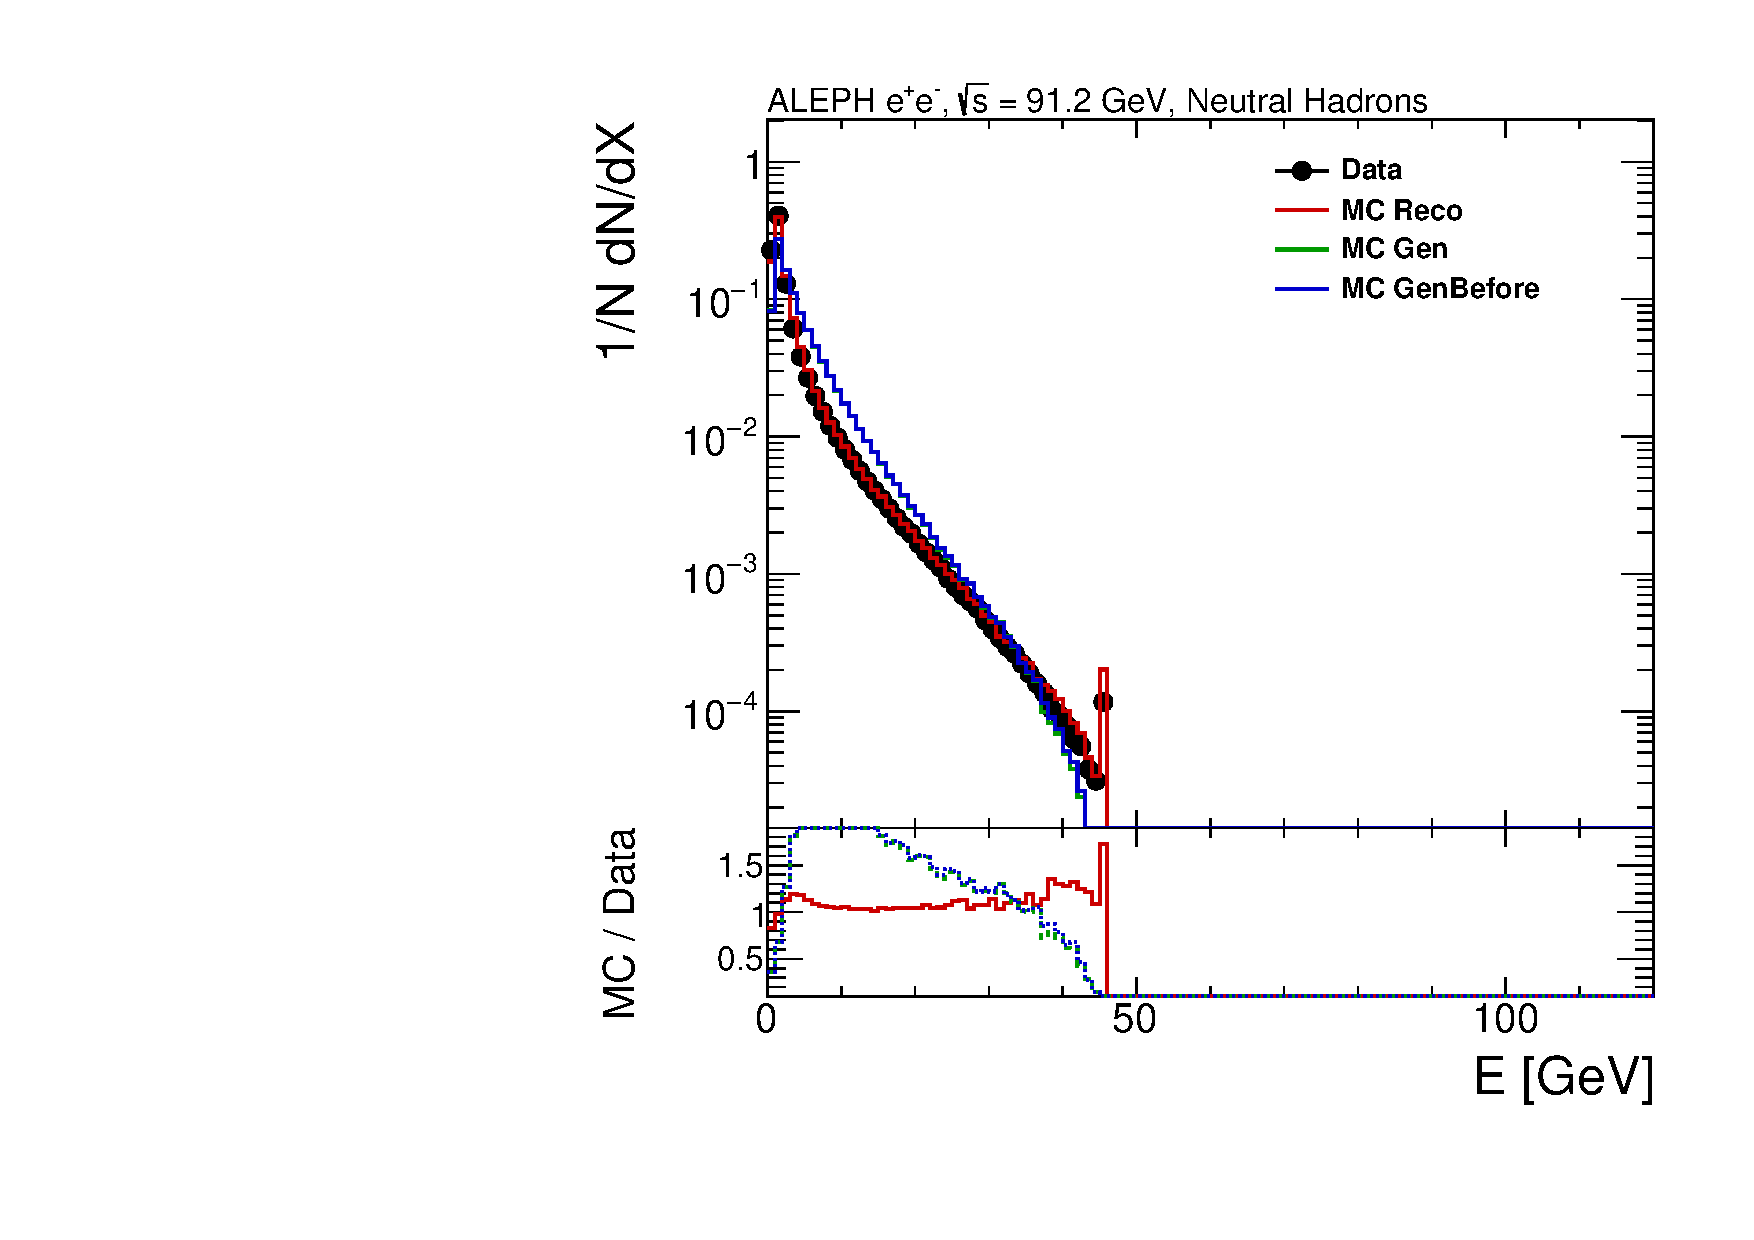
\includegraphics[width=0.495\textwidth]{figures/pwflag5_energy.pdf}
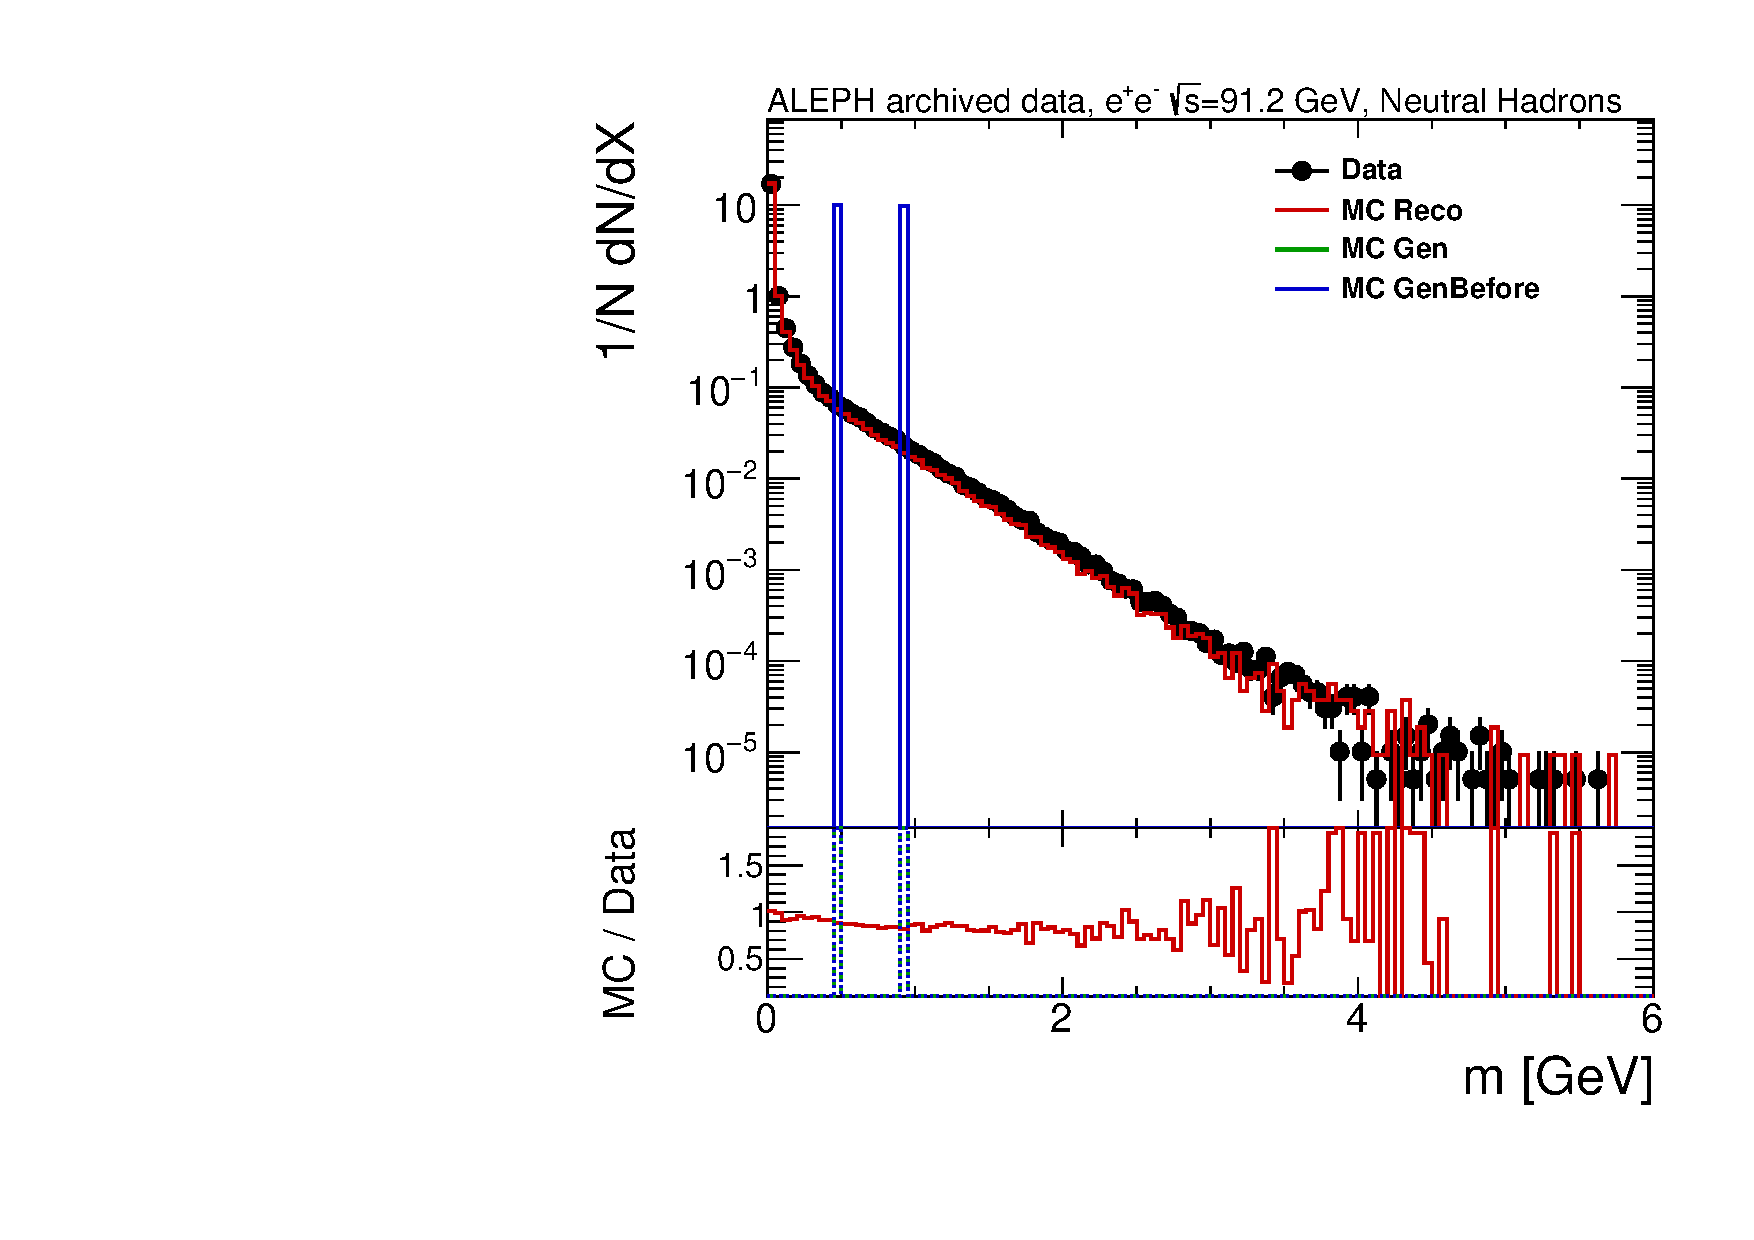
\includegraphics[width=0.495\textwidth]{figures/pwflag5_mass.pdf}
\caption{Complete \texttt{pwflag}=5 kinematic set.}
\label{fig:pwflag5_full}
\end{figure}

\FloatBarrier

\begin{figure}[t!]
\centering
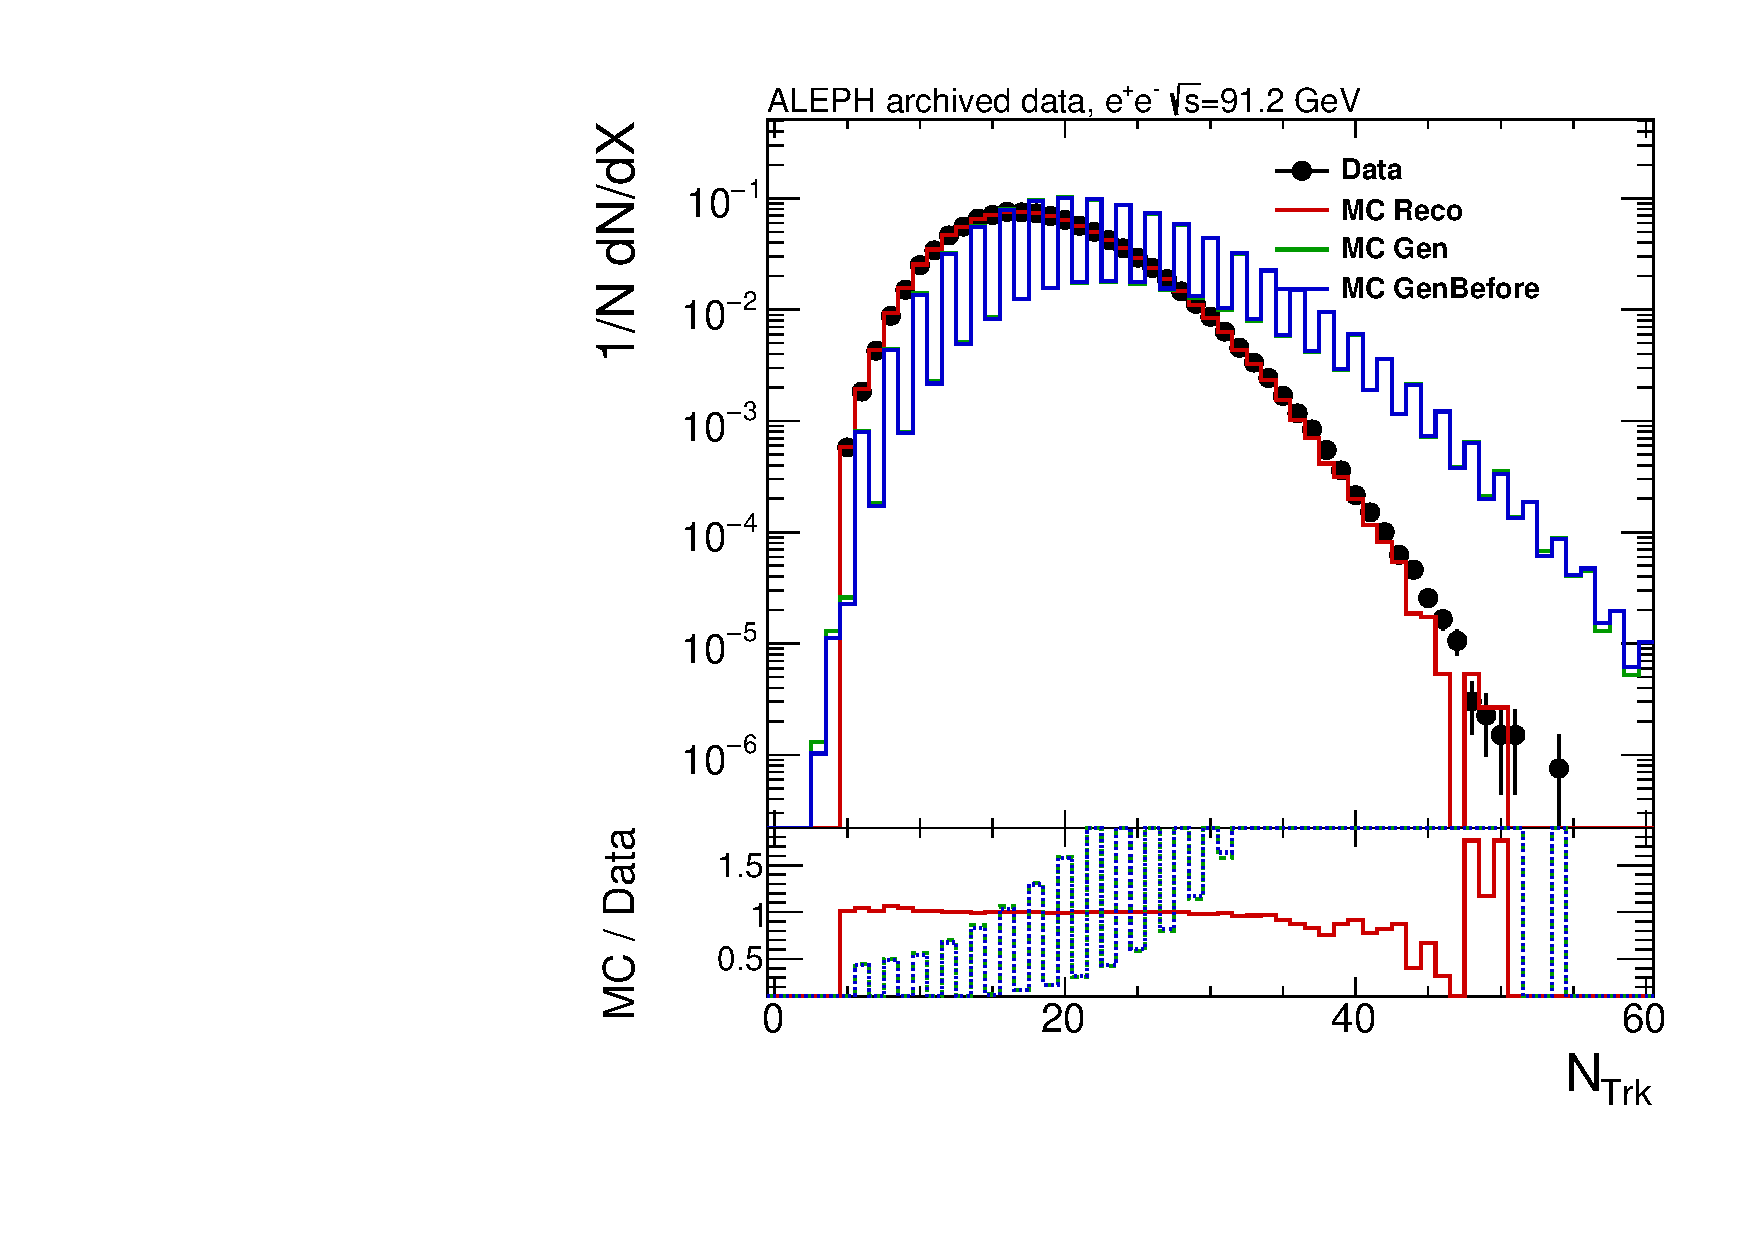
\includegraphics[width=0.495\textwidth]{figures/ntrk.pdf}
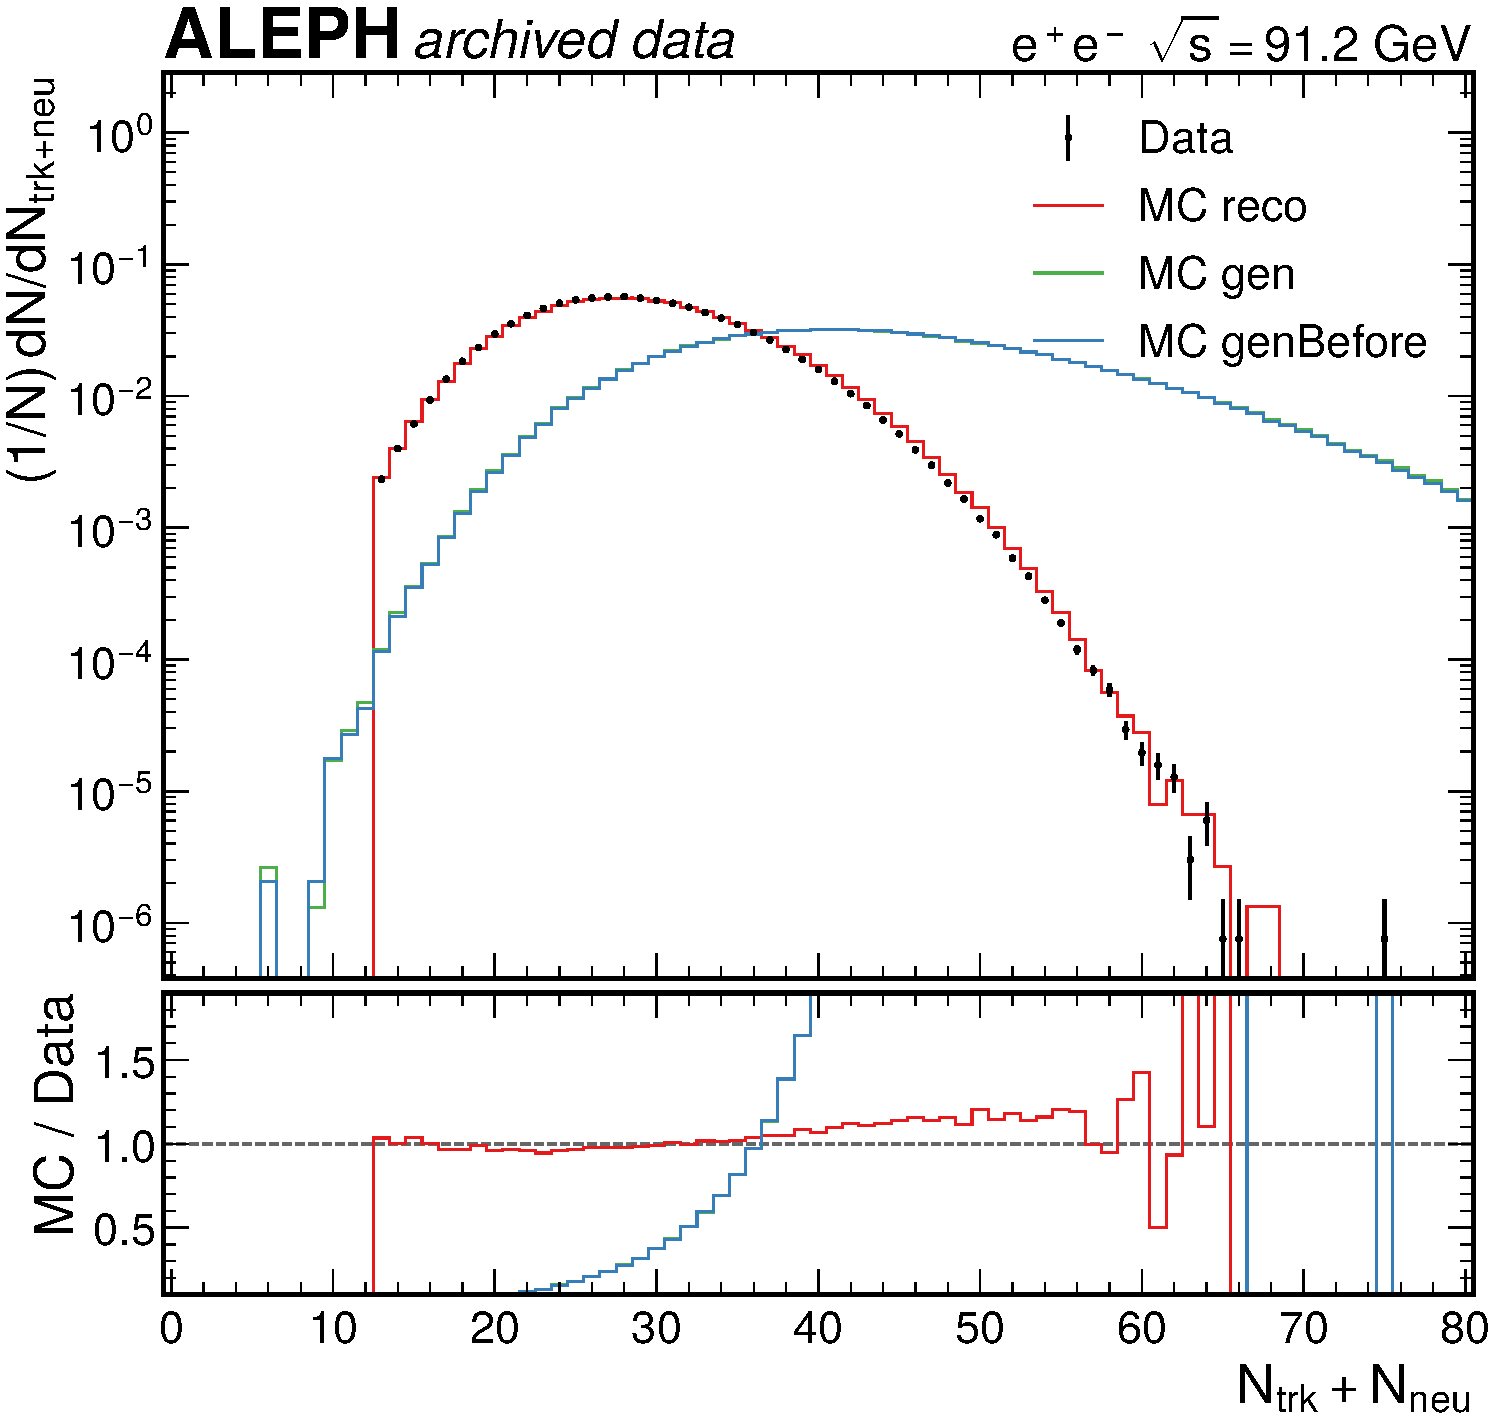
\includegraphics[width=0.495\textwidth]{figures/ntrkPlusNeu.pdf}
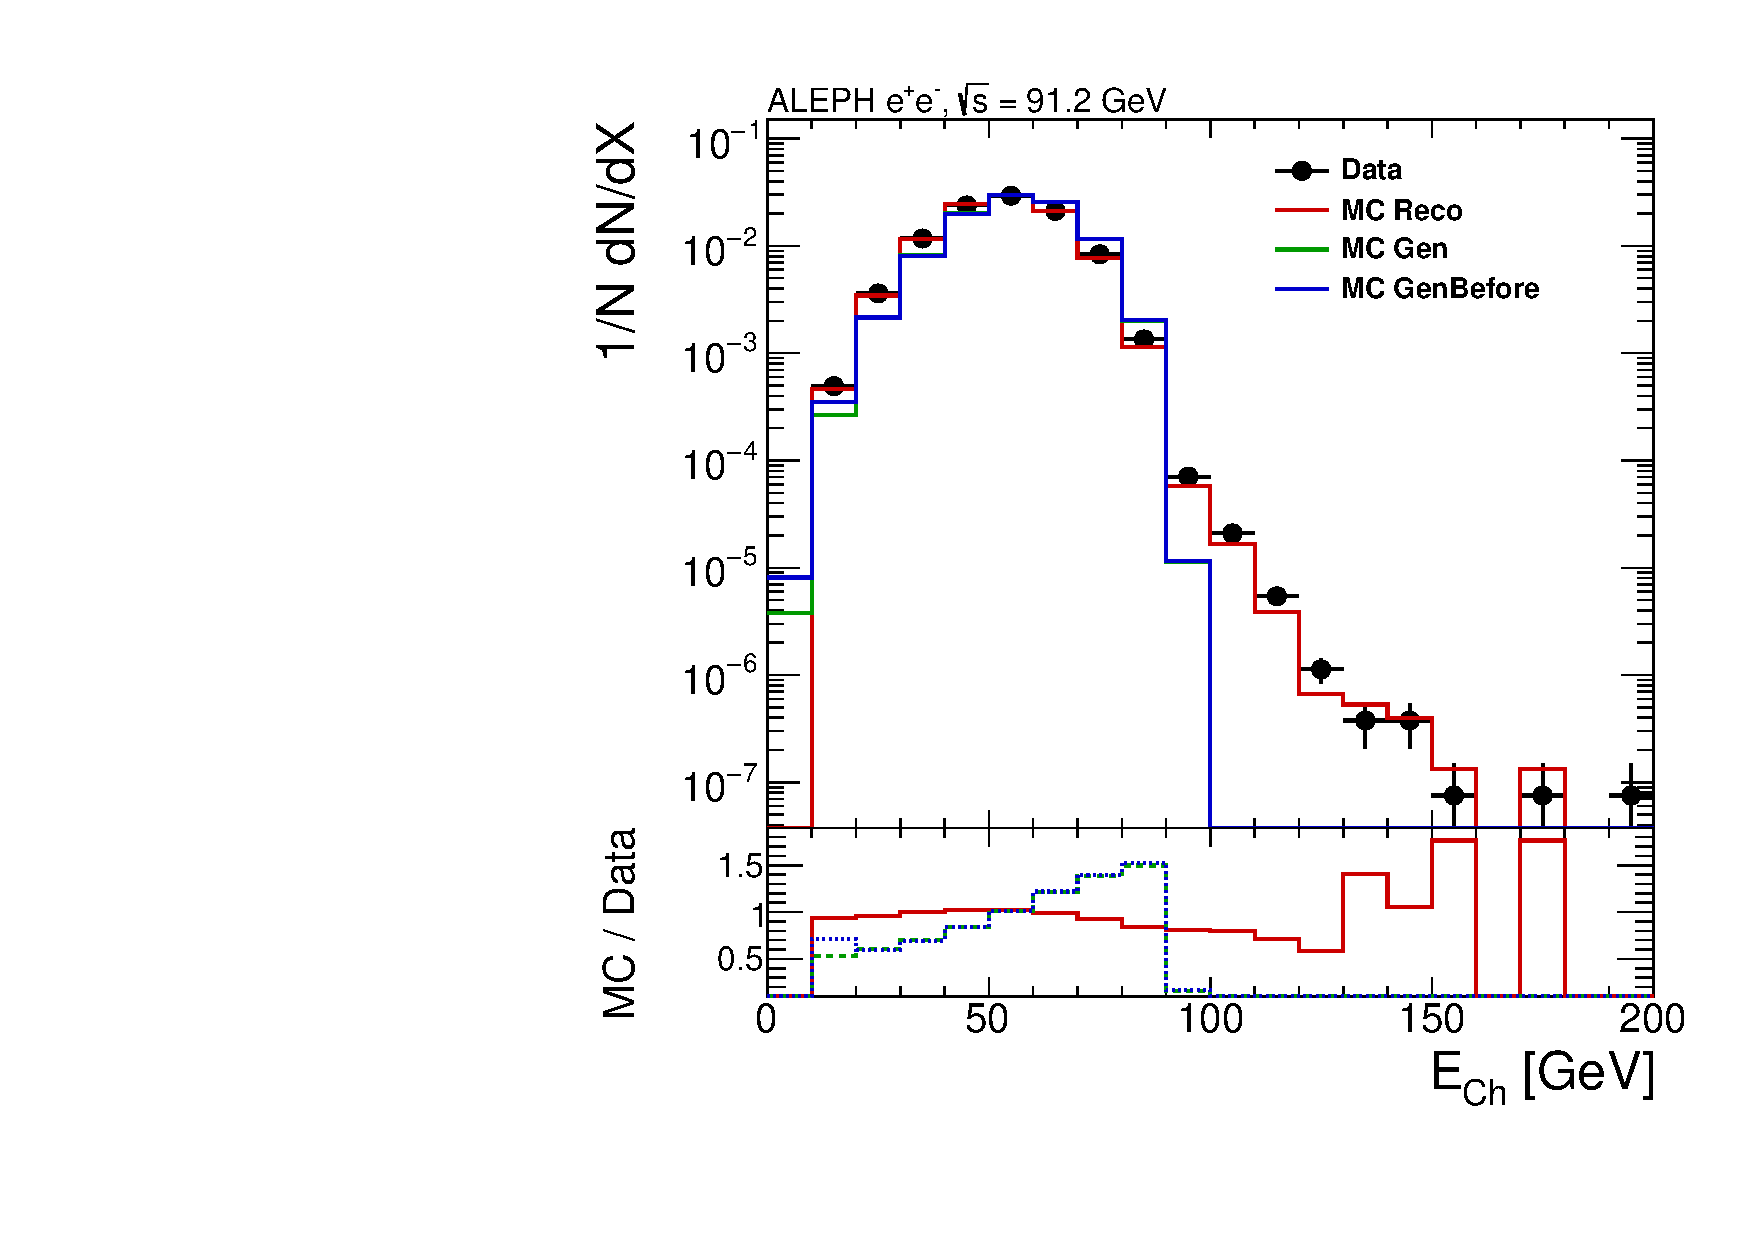
\includegraphics[width=0.495\textwidth]{figures/eCh.pdf}
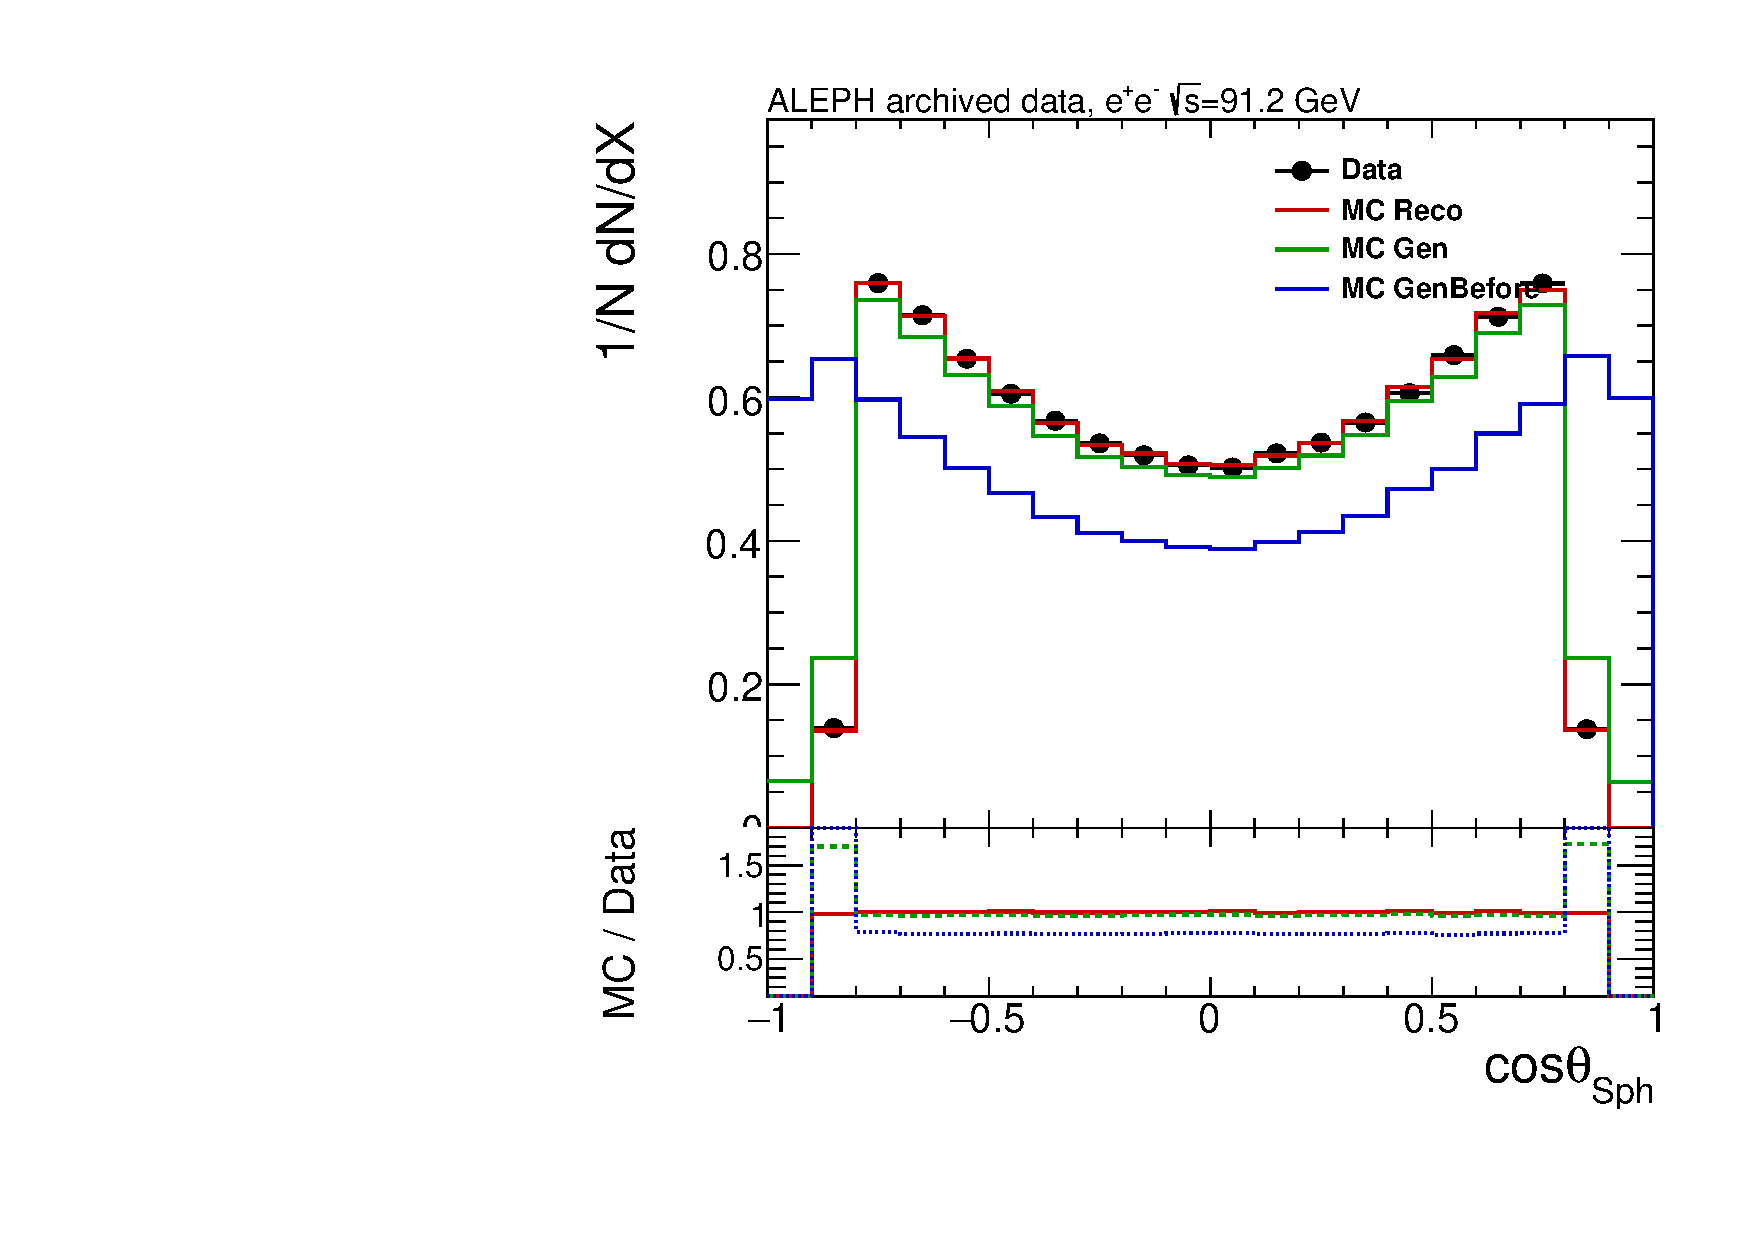
\includegraphics[width=0.495\textwidth]{figures/cosThetaSph.pdf}
\caption{Event-level observables used in the nominal hadronic selection; legends include detector-level data/MC and generator-level references. The MC\,Gen and MC\,GenBefore ratios display an even-odd staggering: generator-level charged multiplicity has an approximately 6:1 even-to-odd ratio (arising from the Z-decay net-charge constraint and the specific ALEPH Pythia~6 particle record), while reconstruction efficiency losses smear individual tracks one at a time and equalise the even/odd balance in data and MC\,Reco.
MC\,Reco is the relevant comparison for the analysis.}
\label{fig:event_selection_observables}
\end{figure}

\FloatBarrier

% \subsection{Event-level selection observables}

% The event-level panels close the logic between object-level selections and the final sample
% entering event-shape reconstruction. $N_{\mathrm{trk}}$ and
% $N_{\mathrm{trk}}+N_{\mathrm{neu}}$ test whether multiplicity thresholds sculpt data and MC in a
% consistent way; this is critical because those same multiplicities enter hadronic-event
% preselection and determine which events contribute to response filling. $E_{\mathrm{Ch}}$ checks
% charged-energy modeling near the hadronic-selection boundary at 15 GeV, and
% $\cos\theta_{\mathrm{Sph}}$ tests whether accepted event topology is similarly contained in
% detector acceptance for data and MC.

% The \texttt{tgen} and \texttt{tgenBefore} samples receive the same particle-level treatment and differ
% only in which events are retained: \texttt{tgen} holds the generator record of the events
% written to the reconstructed after-cut sample, \texttt{tgenBefore} that of all generated
% events, so \texttt{tgen} is a subset. The kinematic selections of
% Sec.~\ref{sec:object_selection} are applied at detector level only, and no additional
% cleaning is applied at generator level. The events
% missing from \texttt{tgen} are removed almost entirely by polar-angle acceptance rather than
% by particle content, so the normalized multiplicity and charged-energy spectra coincide
% through the bulk, separating only in the sparse low-$E_{\mathrm{Ch}}$ tail near the
% charged-energy boundary, and $\cos\theta_{\mathrm{Sph}}$ is the one panel where the curves
% clearly differ. Both generator-level curves also show an even--odd modulation in
% $N_{\mathrm{trk}}$: the charged multiplicity shares the parity of the summed charge of the
% counted particles, which charge conservation makes vanish for most generated events. The
% modulation is absent at detector level, where charged-track inefficiency randomizes the
% parity.

% Overall agreement in the high-statistics regions supports the response-model baseline used for IBU. The visible differences are concentrated in lower-populated tails and near selection boundaries, where statistical fluctuations and detector-response limitations are expected to be larger. These regions are not ignored: their impact is propagated through the experimental systematic program and is reflected in the final uncertainty decomposition.

% \FloatBarrier
% \clearpage
